\documentclass[twoside]{book}

% Packages required by doxygen
\usepackage{fixltx2e}
\usepackage{calc}
\usepackage{doxygen}
\usepackage[export]{adjustbox} % also loads graphicx
\usepackage{graphicx}
\usepackage[utf8]{inputenc}
\usepackage{makeidx}
\usepackage{multicol}
\usepackage{multirow}
\PassOptionsToPackage{warn}{textcomp}
\usepackage{textcomp}
\usepackage[nointegrals]{wasysym}
\usepackage[table]{xcolor}

% Font selection
\usepackage[T1]{fontenc}
\usepackage[scaled=.90]{helvet}
\usepackage{courier}
\usepackage{amssymb}
\usepackage{sectsty}
\renewcommand{\familydefault}{\sfdefault}
\allsectionsfont{%
  \fontseries{bc}\selectfont%
  \color{darkgray}%
}
\renewcommand{\DoxyLabelFont}{%
  \fontseries{bc}\selectfont%
  \color{darkgray}%
}
\newcommand{\+}{\discretionary{\mbox{\scriptsize$\hookleftarrow$}}{}{}}

% Page & text layout
\usepackage{geometry}
\geometry{%
  a4paper,%
  top=2.5cm,%
  bottom=2.5cm,%
  left=2.5cm,%
  right=2.5cm%
}
\tolerance=750
\hfuzz=15pt
\hbadness=750
\setlength{\emergencystretch}{15pt}
\setlength{\parindent}{0cm}
\setlength{\parskip}{3ex plus 2ex minus 2ex}
\makeatletter
\renewcommand{\paragraph}{%
  \@startsection{paragraph}{4}{0ex}{-1.0ex}{1.0ex}{%
    \normalfont\normalsize\bfseries\SS@parafont%
  }%
}
\renewcommand{\subparagraph}{%
  \@startsection{subparagraph}{5}{0ex}{-1.0ex}{1.0ex}{%
    \normalfont\normalsize\bfseries\SS@subparafont%
  }%
}
\makeatother

% Headers & footers
\usepackage{fancyhdr}
\pagestyle{fancyplain}
\fancyhead[LE]{\fancyplain{}{\bfseries\thepage}}
\fancyhead[CE]{\fancyplain{}{}}
\fancyhead[RE]{\fancyplain{}{\bfseries\leftmark}}
\fancyhead[LO]{\fancyplain{}{\bfseries\rightmark}}
\fancyhead[CO]{\fancyplain{}{}}
\fancyhead[RO]{\fancyplain{}{\bfseries\thepage}}
\fancyfoot[LE]{\fancyplain{}{}}
\fancyfoot[CE]{\fancyplain{}{}}
\fancyfoot[RE]{\fancyplain{}{\bfseries\scriptsize Generated by Doxygen }}
\fancyfoot[LO]{\fancyplain{}{\bfseries\scriptsize Generated by Doxygen }}
\fancyfoot[CO]{\fancyplain{}{}}
\fancyfoot[RO]{\fancyplain{}{}}
\renewcommand{\footrulewidth}{0.4pt}
\renewcommand{\chaptermark}[1]{%
  \markboth{#1}{}%
}
\renewcommand{\sectionmark}[1]{%
  \markright{\thesection\ #1}%
}

% Indices & bibliography
\usepackage{natbib}
\usepackage[titles]{tocloft}
\setcounter{tocdepth}{3}
\setcounter{secnumdepth}{5}
\makeindex

% Hyperlinks (required, but should be loaded last)
\usepackage{ifpdf}
\ifpdf
  \usepackage[pdftex,pagebackref=true]{hyperref}
\else
  \usepackage[ps2pdf,pagebackref=true]{hyperref}
\fi
\hypersetup{%
  colorlinks=true,%
  linkcolor=blue,%
  citecolor=blue,%
  unicode%
}

% Custom commands
\newcommand{\clearemptydoublepage}{%
  \newpage{\pagestyle{empty}\cleardoublepage}%
}

\usepackage{caption}
\captionsetup{labelsep=space,justification=centering,font={bf},singlelinecheck=off,skip=4pt,position=top}

%===== C O N T E N T S =====

\begin{document}

% Titlepage & ToC
\hypersetup{pageanchor=false,
             bookmarksnumbered=true,
             pdfencoding=unicode
            }
\pagenumbering{alph}
\begin{titlepage}
\vspace*{7cm}
\begin{center}%
{\Large A\+E\+DA Project }\\
\vspace*{1cm}
{\large Generated by Doxygen 1.8.14}\\
\end{center}
\end{titlepage}
\clearemptydoublepage
\pagenumbering{roman}
\tableofcontents
\clearemptydoublepage
\pagenumbering{arabic}
\hypersetup{pageanchor=true}

%--- Begin generated contents ---
\chapter{Hierarchical Index}
\section{Class Hierarchy}
This inheritance list is sorted roughly, but not completely, alphabetically\+:\begin{DoxyCompactList}
\item \contentsline{section}{Already\+Registered\+Teacher}{\pageref{class_already_registered_teacher}}{}
\item \contentsline{section}{Already\+Registered\+User}{\pageref{class_already_registered_user}}{}
\item \contentsline{section}{Already\+Reserved\+Hours}{\pageref{class_already_reserved_hours}}{}
\begin{DoxyCompactList}
\item \contentsline{section}{End\+Hour\+Inside\+Res}{\pageref{class_end_hour_inside_res}}{}
\item \contentsline{section}{Inside\+Res}{\pageref{class_inside_res}}{}
\item \contentsline{section}{Start\+Hour\+Inside\+Res}{\pageref{class_start_hour_inside_res}}{}
\end{DoxyCompactList}
\item \contentsline{section}{Bad\+Date}{\pageref{class_bad_date}}{}
\item \contentsline{section}{Company}{\pageref{class_company}}{}
\item \contentsline{section}{Court}{\pageref{class_court}}{}
\item \contentsline{section}{Court\+Reserved}{\pageref{class_court_reserved}}{}
\item \contentsline{section}{Date}{\pageref{class_date}}{}
\item \contentsline{section}{Day}{\pageref{class_day}}{}
\item \contentsline{section}{Incorrect\+Month}{\pageref{class_incorrect_month}}{}
\item \contentsline{section}{Invalid\+Age}{\pageref{class_invalid_age}}{}
\item \contentsline{section}{Invalid\+Grade}{\pageref{class_invalid_grade}}{}
\item \contentsline{section}{Invoice}{\pageref{class_invoice}}{}
\item \contentsline{section}{Invoice\+Already\+Exists}{\pageref{class_invoice_already_exists}}{}
\item \contentsline{section}{Invoice\+Not\+Available}{\pageref{class_invoice_not_available}}{}
\item \contentsline{section}{Month}{\pageref{class_month}}{}
\item \contentsline{section}{No\+Teacher\+Registered}{\pageref{class_no_teacher_registered}}{}
\item \contentsline{section}{No\+User\+Registered}{\pageref{class_no_user_registered}}{}
\item \contentsline{section}{Person}{\pageref{class_person}}{}
\begin{DoxyCompactList}
\item \contentsline{section}{Teacher}{\pageref{class_teacher}}{}
\item \contentsline{section}{User}{\pageref{class_user}}{}
\end{DoxyCompactList}
\item \contentsline{section}{Report}{\pageref{class_report}}{}
\item \contentsline{section}{Report\+Already\+Exists}{\pageref{class_report_already_exists}}{}
\item \contentsline{section}{Report\+Not\+Available}{\pageref{class_report_not_available}}{}
\item \contentsline{section}{Reservation}{\pageref{class_reservation}}{}
\begin{DoxyCompactList}
\item \contentsline{section}{Free}{\pageref{class_free}}{}
\item \contentsline{section}{Lesson}{\pageref{class_lesson}}{}
\end{DoxyCompactList}
\item \contentsline{section}{Year}{\pageref{class_year}}{}
\end{DoxyCompactList}

\chapter{Class Index}
\section{Class List}
Here are the classes, structs, unions and interfaces with brief descriptions\+:\begin{DoxyCompactList}
\item\contentsline{section}{\mbox{\hyperlink{class_already_registered_teacher}{Already\+Registered\+Teacher}} }{\pageref{class_already_registered_teacher}}{}
\item\contentsline{section}{\mbox{\hyperlink{class_already_registered_user}{Already\+Registered\+User}} }{\pageref{class_already_registered_user}}{}
\item\contentsline{section}{\mbox{\hyperlink{class_already_reserved_hours}{Already\+Reserved\+Hours}} }{\pageref{class_already_reserved_hours}}{}
\item\contentsline{section}{\mbox{\hyperlink{class_bad_date}{Bad\+Date}} }{\pageref{class_bad_date}}{}
\item\contentsline{section}{\mbox{\hyperlink{class_company}{Company}} }{\pageref{class_company}}{}
\item\contentsline{section}{\mbox{\hyperlink{class_court}{Court}} }{\pageref{class_court}}{}
\item\contentsline{section}{\mbox{\hyperlink{class_court_reserved}{Court\+Reserved}} }{\pageref{class_court_reserved}}{}
\item\contentsline{section}{\mbox{\hyperlink{class_date}{Date}} }{\pageref{class_date}}{}
\item\contentsline{section}{\mbox{\hyperlink{class_day}{Day}} }{\pageref{class_day}}{}
\item\contentsline{section}{\mbox{\hyperlink{class_end_hour_inside_res}{End\+Hour\+Inside\+Res}} }{\pageref{class_end_hour_inside_res}}{}
\item\contentsline{section}{\mbox{\hyperlink{class_free}{Free}} }{\pageref{class_free}}{}
\item\contentsline{section}{\mbox{\hyperlink{class_incorrect_month}{Incorrect\+Month}} }{\pageref{class_incorrect_month}}{}
\item\contentsline{section}{\mbox{\hyperlink{class_inside_res}{Inside\+Res}} }{\pageref{class_inside_res}}{}
\item\contentsline{section}{\mbox{\hyperlink{class_invalid_age}{Invalid\+Age}} }{\pageref{class_invalid_age}}{}
\item\contentsline{section}{\mbox{\hyperlink{class_invalid_grade}{Invalid\+Grade}} }{\pageref{class_invalid_grade}}{}
\item\contentsline{section}{\mbox{\hyperlink{class_invoice}{Invoice}} }{\pageref{class_invoice}}{}
\item\contentsline{section}{\mbox{\hyperlink{class_invoice_already_exists}{Invoice\+Already\+Exists}} }{\pageref{class_invoice_already_exists}}{}
\item\contentsline{section}{\mbox{\hyperlink{class_invoice_not_available}{Invoice\+Not\+Available}} }{\pageref{class_invoice_not_available}}{}
\item\contentsline{section}{\mbox{\hyperlink{class_lesson}{Lesson}} }{\pageref{class_lesson}}{}
\item\contentsline{section}{\mbox{\hyperlink{class_month}{Month}} }{\pageref{class_month}}{}
\item\contentsline{section}{\mbox{\hyperlink{class_no_teacher_registered}{No\+Teacher\+Registered}} }{\pageref{class_no_teacher_registered}}{}
\item\contentsline{section}{\mbox{\hyperlink{class_no_user_registered}{No\+User\+Registered}} }{\pageref{class_no_user_registered}}{}
\item\contentsline{section}{\mbox{\hyperlink{class_person}{Person}} }{\pageref{class_person}}{}
\item\contentsline{section}{\mbox{\hyperlink{class_report}{Report}} }{\pageref{class_report}}{}
\item\contentsline{section}{\mbox{\hyperlink{class_report_already_exists}{Report\+Already\+Exists}} }{\pageref{class_report_already_exists}}{}
\item\contentsline{section}{\mbox{\hyperlink{class_report_not_available}{Report\+Not\+Available}} }{\pageref{class_report_not_available}}{}
\item\contentsline{section}{\mbox{\hyperlink{class_reservation}{Reservation}} }{\pageref{class_reservation}}{}
\item\contentsline{section}{\mbox{\hyperlink{class_start_hour_inside_res}{Start\+Hour\+Inside\+Res}} }{\pageref{class_start_hour_inside_res}}{}
\item\contentsline{section}{\mbox{\hyperlink{class_teacher}{Teacher}} }{\pageref{class_teacher}}{}
\item\contentsline{section}{\mbox{\hyperlink{class_user}{User}} }{\pageref{class_user}}{}
\item\contentsline{section}{\mbox{\hyperlink{class_year}{Year}} }{\pageref{class_year}}{}
\end{DoxyCompactList}

\chapter{Class Documentation}
\hypertarget{class_already_registered_teacher}{}\section{Already\+Registered\+Teacher Class Reference}
\label{class_already_registered_teacher}\index{Already\+Registered\+Teacher@{Already\+Registered\+Teacher}}


{\ttfamily \#include $<$Company.\+h$>$}

\subsection*{Public Member Functions}
\begin{DoxyCompactItemize}
\item 
\mbox{\hyperlink{class_already_registered_teacher_ab6bdaf12fd3147274d10f6595d424a8e}{Already\+Registered\+Teacher}} (std\+::string name)
\item 
std\+::string \mbox{\hyperlink{class_already_registered_teacher_a3d7912fc2aa048ad661db2fa82f17d35}{what}} () const
\end{DoxyCompactItemize}


\subsection{Detailed Description}
When that name is already in the system 

\subsection{Constructor \& Destructor Documentation}
\mbox{\Hypertarget{class_already_registered_teacher_ab6bdaf12fd3147274d10f6595d424a8e}\label{class_already_registered_teacher_ab6bdaf12fd3147274d10f6595d424a8e}} 
\index{Already\+Registered\+Teacher@{Already\+Registered\+Teacher}!Already\+Registered\+Teacher@{Already\+Registered\+Teacher}}
\index{Already\+Registered\+Teacher@{Already\+Registered\+Teacher}!Already\+Registered\+Teacher@{Already\+Registered\+Teacher}}
\subsubsection{\texorpdfstring{Already\+Registered\+Teacher()}{AlreadyRegisteredTeacher()}}
{\footnotesize\ttfamily Already\+Registered\+Teacher\+::\+Already\+Registered\+Teacher (\begin{DoxyParamCaption}\item[{std\+::string}]{name }\end{DoxyParamCaption})\hspace{0.3cm}{\ttfamily [inline]}}



\subsection{Member Function Documentation}
\mbox{\Hypertarget{class_already_registered_teacher_a3d7912fc2aa048ad661db2fa82f17d35}\label{class_already_registered_teacher_a3d7912fc2aa048ad661db2fa82f17d35}} 
\index{Already\+Registered\+Teacher@{Already\+Registered\+Teacher}!what@{what}}
\index{what@{what}!Already\+Registered\+Teacher@{Already\+Registered\+Teacher}}
\subsubsection{\texorpdfstring{what()}{what()}}
{\footnotesize\ttfamily string Already\+Registered\+Teacher\+::what (\begin{DoxyParamCaption}{ }\end{DoxyParamCaption}) const}



The documentation for this class was generated from the following files\+:\begin{DoxyCompactItemize}
\item 
\mbox{\hyperlink{_company_8h}{Company.\+h}}\item 
\mbox{\hyperlink{_company_8cpp}{Company.\+cpp}}\end{DoxyCompactItemize}

\hypertarget{class_already_registered_user}{}\section{Already\+Registered\+User Class Reference}
\label{class_already_registered_user}\index{Already\+Registered\+User@{Already\+Registered\+User}}


{\ttfamily \#include $<$Company.\+h$>$}

\subsection*{Public Member Functions}
\begin{DoxyCompactItemize}
\item 
\mbox{\hyperlink{class_already_registered_user_a8daf190044233235e28f8c53e922fabd}{Already\+Registered\+User}} (std\+::string name)
\item 
std\+::string \mbox{\hyperlink{class_already_registered_user_ae9f46091d164347cc12e45591d86d5a5}{what}} () const
\end{DoxyCompactItemize}


\subsection{Detailed Description}
When that name is already in the system 

\subsection{Constructor \& Destructor Documentation}
\mbox{\Hypertarget{class_already_registered_user_a8daf190044233235e28f8c53e922fabd}\label{class_already_registered_user_a8daf190044233235e28f8c53e922fabd}} 
\index{Already\+Registered\+User@{Already\+Registered\+User}!Already\+Registered\+User@{Already\+Registered\+User}}
\index{Already\+Registered\+User@{Already\+Registered\+User}!Already\+Registered\+User@{Already\+Registered\+User}}
\subsubsection{\texorpdfstring{Already\+Registered\+User()}{AlreadyRegisteredUser()}}
{\footnotesize\ttfamily Already\+Registered\+User\+::\+Already\+Registered\+User (\begin{DoxyParamCaption}\item[{std\+::string}]{name }\end{DoxyParamCaption})\hspace{0.3cm}{\ttfamily [inline]}}



\subsection{Member Function Documentation}
\mbox{\Hypertarget{class_already_registered_user_ae9f46091d164347cc12e45591d86d5a5}\label{class_already_registered_user_ae9f46091d164347cc12e45591d86d5a5}} 
\index{Already\+Registered\+User@{Already\+Registered\+User}!what@{what}}
\index{what@{what}!Already\+Registered\+User@{Already\+Registered\+User}}
\subsubsection{\texorpdfstring{what()}{what()}}
{\footnotesize\ttfamily string Already\+Registered\+User\+::what (\begin{DoxyParamCaption}{ }\end{DoxyParamCaption}) const}



The documentation for this class was generated from the following files\+:\begin{DoxyCompactItemize}
\item 
\mbox{\hyperlink{_company_8h}{Company.\+h}}\item 
\mbox{\hyperlink{_company_8cpp}{Company.\+cpp}}\end{DoxyCompactItemize}

\hypertarget{class_already_reserved_hours}{}\section{Already\+Reserved\+Hours Class Reference}
\label{class_already_reserved_hours}\index{Already\+Reserved\+Hours@{Already\+Reserved\+Hours}}


{\ttfamily \#include $<$Person.\+h$>$}

Inheritance diagram for Already\+Reserved\+Hours\+:\begin{figure}[H]
\begin{center}
\leavevmode
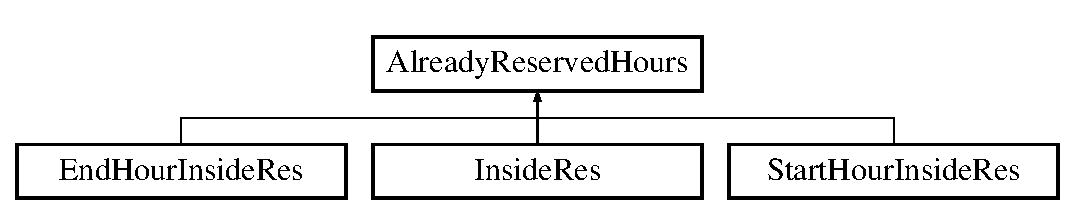
\includegraphics[height=2.000000cm]{class_already_reserved_hours}
\end{center}
\end{figure}
\subsection*{Public Member Functions}
\begin{DoxyCompactItemize}
\item 
\mbox{\hyperlink{class_already_reserved_hours_a3602604e7295f0a54eb68079c3b2917b}{Already\+Reserved\+Hours}} ()
\item 
virtual std\+::string \mbox{\hyperlink{class_already_reserved_hours_a69081ef7e75aa68b9aa5c75d02fe2194}{what}} () const
\end{DoxyCompactItemize}


\subsection{Detailed Description}
When there is already a reservation at that time 

\subsection{Constructor \& Destructor Documentation}
\mbox{\Hypertarget{class_already_reserved_hours_a3602604e7295f0a54eb68079c3b2917b}\label{class_already_reserved_hours_a3602604e7295f0a54eb68079c3b2917b}} 
\index{Already\+Reserved\+Hours@{Already\+Reserved\+Hours}!Already\+Reserved\+Hours@{Already\+Reserved\+Hours}}
\index{Already\+Reserved\+Hours@{Already\+Reserved\+Hours}!Already\+Reserved\+Hours@{Already\+Reserved\+Hours}}
\subsubsection{\texorpdfstring{Already\+Reserved\+Hours()}{AlreadyReservedHours()}}
{\footnotesize\ttfamily Already\+Reserved\+Hours\+::\+Already\+Reserved\+Hours (\begin{DoxyParamCaption}{ }\end{DoxyParamCaption})\hspace{0.3cm}{\ttfamily [inline]}}



\subsection{Member Function Documentation}
\mbox{\Hypertarget{class_already_reserved_hours_a69081ef7e75aa68b9aa5c75d02fe2194}\label{class_already_reserved_hours_a69081ef7e75aa68b9aa5c75d02fe2194}} 
\index{Already\+Reserved\+Hours@{Already\+Reserved\+Hours}!what@{what}}
\index{what@{what}!Already\+Reserved\+Hours@{Already\+Reserved\+Hours}}
\subsubsection{\texorpdfstring{what()}{what()}}
{\footnotesize\ttfamily virtual std\+::string Already\+Reserved\+Hours\+::what (\begin{DoxyParamCaption}{ }\end{DoxyParamCaption}) const\hspace{0.3cm}{\ttfamily [inline]}, {\ttfamily [virtual]}}



Reimplemented in \mbox{\hyperlink{class_start_hour_inside_res_a90b45cf2a2d4f0adcf7d9f650bee1574}{Start\+Hour\+Inside\+Res}}, \mbox{\hyperlink{class_end_hour_inside_res_afee9514b15c167847bc55ebe833076ff}{End\+Hour\+Inside\+Res}}, and \mbox{\hyperlink{class_inside_res_af8e96688976739ec91630a369d4b94e7}{Inside\+Res}}.



The documentation for this class was generated from the following file\+:\begin{DoxyCompactItemize}
\item 
\mbox{\hyperlink{_person_8h}{Person.\+h}}\end{DoxyCompactItemize}

\hypertarget{class_bad_date}{}\section{Bad\+Date Class Reference}
\label{class_bad_date}\index{Bad\+Date@{Bad\+Date}}


{\ttfamily \#include $<$Date.\+h$>$}

\subsection*{Public Member Functions}
\begin{DoxyCompactItemize}
\item 
std\+::string \mbox{\hyperlink{class_bad_date_a50ea387c6301cf0279943fdc5a7db02d}{what}} ()
\end{DoxyCompactItemize}


\subsection{Detailed Description}
When a date is invalid 

\subsection{Member Function Documentation}
\mbox{\Hypertarget{class_bad_date_a50ea387c6301cf0279943fdc5a7db02d}\label{class_bad_date_a50ea387c6301cf0279943fdc5a7db02d}} 
\index{Bad\+Date@{Bad\+Date}!what@{what}}
\index{what@{what}!Bad\+Date@{Bad\+Date}}
\subsubsection{\texorpdfstring{what()}{what()}}
{\footnotesize\ttfamily std\+::string Bad\+Date\+::what (\begin{DoxyParamCaption}{ }\end{DoxyParamCaption})}



The documentation for this class was generated from the following files\+:\begin{DoxyCompactItemize}
\item 
\mbox{\hyperlink{_date_8h}{Date.\+h}}\item 
\mbox{\hyperlink{_date_8cpp}{Date.\+cpp}}\end{DoxyCompactItemize}

\hypertarget{class_company}{}\section{Company Class Reference}
\label{class_company}\index{Company@{Company}}


{\ttfamily \#include $<$Company.\+h$>$}

\subsection*{Public Member Functions}
\begin{DoxyCompactItemize}
\item 
\mbox{\hyperlink{class_company_ac97cf640176971922a434b766627774f}{Company}} (double card\+Value, int year)
\begin{DoxyCompactList}\small\item\em Class Constructor. \end{DoxyCompactList}\item 
int \mbox{\hyperlink{class_company_a837fd39a8f03c20a3ceb8617410956b7}{get\+Max\+User}} () const
\begin{DoxyCompactList}\small\item\em Getter of the maxium numbr of users. \end{DoxyCompactList}\item 
\mbox{\Hypertarget{class_company_a10770d690a59f9b4d9f84de6d0f527c9}\label{class_company_a10770d690a59f9b4d9f84de6d0f527c9}} 
void \mbox{\hyperlink{class_company_a10770d690a59f9b4d9f84de6d0f527c9}{create\+Court}} ()
\begin{DoxyCompactList}\small\item\em Creating a new \mbox{\hyperlink{class_court}{Court}}. \end{DoxyCompactList}\item 
std\+::vector$<$ \mbox{\hyperlink{class_court}{Court}} $>$ \mbox{\hyperlink{class_company_afa0ab125a0ba718fe2c13802fe1703be}{get\+Courts}} ()
\begin{DoxyCompactList}\small\item\em Getter of the current Courts. \end{DoxyCompactList}\item 
std\+::vector$<$ \mbox{\hyperlink{class_user}{User}} $>$ \mbox{\hyperlink{class_company_a6f6a3dbf24278f5e1395d123d5812f33}{get\+Users}} ()
\begin{DoxyCompactList}\small\item\em Getter of the current Users. \end{DoxyCompactList}\item 
std\+::vector$<$ \mbox{\hyperlink{class_teacher}{Teacher}} $>$ \mbox{\hyperlink{class_company_a000159ce012318a6edf0335447ad8bde}{get\+Teachers}} ()
\begin{DoxyCompactList}\small\item\em Getter of the current Teachers. \end{DoxyCompactList}\item 
int \mbox{\hyperlink{class_company_ad3fc4daf4b94e0156f05049eab8ff52d}{get\+User}} (std\+::string user\+Name)
\begin{DoxyCompactList}\small\item\em Getting a specific users. \end{DoxyCompactList}\item 
bool \mbox{\hyperlink{class_company_a0ab3ff0ea443cc20fd1ea99e5d8725c9}{make\+Lesson}} (int month, int day, double starting\+Hour, std\+::string user\+Name, std\+::string teacher\+Name)
\begin{DoxyCompactList}\small\item\em Reserving the \mbox{\hyperlink{class_court}{Court}}, \mbox{\hyperlink{class_user}{User}} and \mbox{\hyperlink{class_teacher}{Teacher}} for a new \mbox{\hyperlink{class_lesson}{Lesson}}. \end{DoxyCompactList}\item 
bool \mbox{\hyperlink{class_company_a56fa75dd66690eae0853a3f3278220e3}{make\+Free}} (int month, int day, double starting\+Hour, int duration, std\+::string username)
\begin{DoxyCompactList}\small\item\em Reserving the \mbox{\hyperlink{class_court}{Court}}, \mbox{\hyperlink{class_user}{User}} and \mbox{\hyperlink{class_teacher}{Teacher}} for a new \mbox{\hyperlink{class_reservation}{Reservation}}. \end{DoxyCompactList}\item 
bool \mbox{\hyperlink{class_company_a94383e957bfa622949f1e577a325a1d5}{register\+User}} (std\+::string name, int age, bool is\+Gold, std\+::string gender)
\begin{DoxyCompactList}\small\item\em Register a new \mbox{\hyperlink{class_user}{User}} to the system. \end{DoxyCompactList}\item 
bool \mbox{\hyperlink{class_company_afd7f0c326672c6bb6a23d5921503bc0d}{register\+Teacher}} (std\+::string teacher\+Name, int age, std\+::string gender)
\begin{DoxyCompactList}\small\item\em Register a new \mbox{\hyperlink{class_teacher}{Teacher}} to the system. \end{DoxyCompactList}\item 
bool \mbox{\hyperlink{class_company_a6fe989c0c3da3db723e37f6a71378fd4}{make\+User\+Report}} (int month, std\+::string user\+Name, std\+::string teacher\+Name, int grade, std\+::string addcomm)
\begin{DoxyCompactList}\small\item\em Make a \mbox{\hyperlink{class_report}{Report}} for a specific user. \end{DoxyCompactList}\item 
bool \mbox{\hyperlink{class_company_a0d3e4de51625c91610516fba5aac7acf}{make\+User\+Invoice}} (std\+::string user\+Name, int month, std\+::vector$<$ \mbox{\hyperlink{class_reservation}{Reservation}} $\ast$$>$ reservs)
\begin{DoxyCompactList}\small\item\em Make an \mbox{\hyperlink{class_invoice}{Invoice}} for a specific user. \end{DoxyCompactList}\item 
bool \mbox{\hyperlink{class_company_a2c00c88b245aef0e0e52864b585f8f6b}{show\+Report}} (std\+::string name, int month)
\begin{DoxyCompactList}\small\item\em Method to show a specific \mbox{\hyperlink{class_report}{Report}}. \end{DoxyCompactList}\item 
bool \mbox{\hyperlink{class_company_ad3d0ab0209f13ca48a83df34564ef055}{show\+Invoice}} (std\+::string name, int month)
\begin{DoxyCompactList}\small\item\em Method to show a specific \mbox{\hyperlink{class_invoice}{Invoice}}. \end{DoxyCompactList}\item 
void \mbox{\hyperlink{class_company_ac03f62f1accf21eb445a7aa5731b1199}{store\+Info}} (std\+::ofstream \&outfile, int identation)
\begin{DoxyCompactList}\small\item\em Store in the information of the \mbox{\hyperlink{class_company}{Company}} to a file. \end{DoxyCompactList}\item 
void \mbox{\hyperlink{class_company_aa2885e87763b9fa599ec4935d3ded6cc}{indent}} (std\+::ofstream \&outfile, int identation)
\begin{DoxyCompactList}\small\item\em Indenting the file. \end{DoxyCompactList}\end{DoxyCompactItemize}


\subsection{Detailed Description}
The company itself, operation all of the rest 

\subsection{Constructor \& Destructor Documentation}
\mbox{\Hypertarget{class_company_ac97cf640176971922a434b766627774f}\label{class_company_ac97cf640176971922a434b766627774f}} 
\index{Company@{Company}!Company@{Company}}
\index{Company@{Company}!Company@{Company}}
\subsubsection{\texorpdfstring{Company()}{Company()}}
{\footnotesize\ttfamily Company\+::\+Company (\begin{DoxyParamCaption}\item[{double}]{card\+Value,  }\item[{int}]{year }\end{DoxyParamCaption})}



Class Constructor. 


\begin{DoxyParams}{Parameters}
{\em card\+Value} & -\/ the value of the Gold Card \\
\hline
{\em year} & -\/ Current year \\
\hline
\end{DoxyParams}


\subsection{Member Function Documentation}
\mbox{\Hypertarget{class_company_afa0ab125a0ba718fe2c13802fe1703be}\label{class_company_afa0ab125a0ba718fe2c13802fe1703be}} 
\index{Company@{Company}!get\+Courts@{get\+Courts}}
\index{get\+Courts@{get\+Courts}!Company@{Company}}
\subsubsection{\texorpdfstring{get\+Courts()}{getCourts()}}
{\footnotesize\ttfamily vector$<$ \mbox{\hyperlink{class_court}{Court}} $>$ Company\+::get\+Courts (\begin{DoxyParamCaption}{ }\end{DoxyParamCaption})}



Getter of the current Courts. 

\begin{DoxyReturn}{Returns}
vector of Courts 
\end{DoxyReturn}
\mbox{\Hypertarget{class_company_a837fd39a8f03c20a3ceb8617410956b7}\label{class_company_a837fd39a8f03c20a3ceb8617410956b7}} 
\index{Company@{Company}!get\+Max\+User@{get\+Max\+User}}
\index{get\+Max\+User@{get\+Max\+User}!Company@{Company}}
\subsubsection{\texorpdfstring{get\+Max\+User()}{getMaxUser()}}
{\footnotesize\ttfamily int Company\+::get\+Max\+User (\begin{DoxyParamCaption}{ }\end{DoxyParamCaption}) const}



Getter of the maxium numbr of users. 

\begin{DoxyReturn}{Returns}
number of max Users 
\end{DoxyReturn}
\mbox{\Hypertarget{class_company_a000159ce012318a6edf0335447ad8bde}\label{class_company_a000159ce012318a6edf0335447ad8bde}} 
\index{Company@{Company}!get\+Teachers@{get\+Teachers}}
\index{get\+Teachers@{get\+Teachers}!Company@{Company}}
\subsubsection{\texorpdfstring{get\+Teachers()}{getTeachers()}}
{\footnotesize\ttfamily vector$<$ \mbox{\hyperlink{class_teacher}{Teacher}} $>$ Company\+::get\+Teachers (\begin{DoxyParamCaption}{ }\end{DoxyParamCaption})}



Getter of the current Teachers. 

\begin{DoxyReturn}{Returns}
vector of Teachers 
\end{DoxyReturn}
\mbox{\Hypertarget{class_company_ad3fc4daf4b94e0156f05049eab8ff52d}\label{class_company_ad3fc4daf4b94e0156f05049eab8ff52d}} 
\index{Company@{Company}!get\+User@{get\+User}}
\index{get\+User@{get\+User}!Company@{Company}}
\subsubsection{\texorpdfstring{get\+User()}{getUser()}}
{\footnotesize\ttfamily int Company\+::get\+User (\begin{DoxyParamCaption}\item[{std\+::string}]{user\+Name }\end{DoxyParamCaption})}



Getting a specific users. 


\begin{DoxyParams}{Parameters}
{\em user\+Name} & -\/ the name of the user \\
\hline
\end{DoxyParams}
\begin{DoxyReturn}{Returns}
return the index of where he is 
\end{DoxyReturn}
\mbox{\Hypertarget{class_company_a6f6a3dbf24278f5e1395d123d5812f33}\label{class_company_a6f6a3dbf24278f5e1395d123d5812f33}} 
\index{Company@{Company}!get\+Users@{get\+Users}}
\index{get\+Users@{get\+Users}!Company@{Company}}
\subsubsection{\texorpdfstring{get\+Users()}{getUsers()}}
{\footnotesize\ttfamily vector$<$ \mbox{\hyperlink{class_user}{User}} $>$ Company\+::get\+Users (\begin{DoxyParamCaption}{ }\end{DoxyParamCaption})}



Getter of the current Users. 

\begin{DoxyReturn}{Returns}
vector of Users 
\end{DoxyReturn}
\mbox{\Hypertarget{class_company_aa2885e87763b9fa599ec4935d3ded6cc}\label{class_company_aa2885e87763b9fa599ec4935d3ded6cc}} 
\index{Company@{Company}!indent@{indent}}
\index{indent@{indent}!Company@{Company}}
\subsubsection{\texorpdfstring{indent()}{indent()}}
{\footnotesize\ttfamily void Company\+::indent (\begin{DoxyParamCaption}\item[{std\+::ofstream \&}]{outfile,  }\item[{int}]{identation }\end{DoxyParamCaption})}



Indenting the file. 


\begin{DoxyParams}{Parameters}
{\em outfile} & -\/ the file to write information \\
\hline
{\em indent} & -\/ current indentation \\
\hline
\end{DoxyParams}
\mbox{\Hypertarget{class_company_a56fa75dd66690eae0853a3f3278220e3}\label{class_company_a56fa75dd66690eae0853a3f3278220e3}} 
\index{Company@{Company}!make\+Free@{make\+Free}}
\index{make\+Free@{make\+Free}!Company@{Company}}
\subsubsection{\texorpdfstring{make\+Free()}{makeFree()}}
{\footnotesize\ttfamily bool Company\+::make\+Free (\begin{DoxyParamCaption}\item[{int}]{month,  }\item[{int}]{day,  }\item[{double}]{starting\+Hour,  }\item[{int}]{duration,  }\item[{std\+::string}]{username }\end{DoxyParamCaption})}



Reserving the \mbox{\hyperlink{class_court}{Court}}, \mbox{\hyperlink{class_user}{User}} and \mbox{\hyperlink{class_teacher}{Teacher}} for a new \mbox{\hyperlink{class_reservation}{Reservation}}. 


\begin{DoxyParams}{Parameters}
{\em month} & -\/ the month of the lesson \\
\hline
{\em day} & -\/ the day of the lesson \\
\hline
{\em starting\+Hour} & -\/ the starting Hour for it \\
\hline
{\em user\+Name} & -\/ the name of the \mbox{\hyperlink{class_user}{User}} \\
\hline
{\em duration} & -\/ the duration it \\
\hline
\end{DoxyParams}
\begin{DoxyReturn}{Returns}
if it was successful created 
\end{DoxyReturn}
\mbox{\Hypertarget{class_company_a0ab3ff0ea443cc20fd1ea99e5d8725c9}\label{class_company_a0ab3ff0ea443cc20fd1ea99e5d8725c9}} 
\index{Company@{Company}!make\+Lesson@{make\+Lesson}}
\index{make\+Lesson@{make\+Lesson}!Company@{Company}}
\subsubsection{\texorpdfstring{make\+Lesson()}{makeLesson()}}
{\footnotesize\ttfamily bool Company\+::make\+Lesson (\begin{DoxyParamCaption}\item[{int}]{month,  }\item[{int}]{day,  }\item[{double}]{starting\+Hour,  }\item[{std\+::string}]{user\+Name,  }\item[{std\+::string}]{teacher\+Name }\end{DoxyParamCaption})}



Reserving the \mbox{\hyperlink{class_court}{Court}}, \mbox{\hyperlink{class_user}{User}} and \mbox{\hyperlink{class_teacher}{Teacher}} for a new \mbox{\hyperlink{class_lesson}{Lesson}}. 


\begin{DoxyParams}{Parameters}
{\em month} & -\/ the month of the lesson \\
\hline
{\em day} & -\/ the day of the lesson \\
\hline
{\em starting\+Hour} & -\/ the starting Hour for it \\
\hline
{\em user\+Name} & -\/ the name of the \mbox{\hyperlink{class_user}{User}} \\
\hline
{\em teacher\+Name} & -\/ the name of the \mbox{\hyperlink{class_teacher}{Teacher}} \\
\hline
\end{DoxyParams}
\begin{DoxyReturn}{Returns}
if it was successful created 
\end{DoxyReturn}
\mbox{\Hypertarget{class_company_a0d3e4de51625c91610516fba5aac7acf}\label{class_company_a0d3e4de51625c91610516fba5aac7acf}} 
\index{Company@{Company}!make\+User\+Invoice@{make\+User\+Invoice}}
\index{make\+User\+Invoice@{make\+User\+Invoice}!Company@{Company}}
\subsubsection{\texorpdfstring{make\+User\+Invoice()}{makeUserInvoice()}}
{\footnotesize\ttfamily bool Company\+::make\+User\+Invoice (\begin{DoxyParamCaption}\item[{std\+::string}]{user\+Name,  }\item[{int}]{month,  }\item[{std\+::vector$<$ \mbox{\hyperlink{class_reservation}{Reservation}} $\ast$$>$}]{reservs }\end{DoxyParamCaption})}



Make an \mbox{\hyperlink{class_invoice}{Invoice}} for a specific user. 


\begin{DoxyParams}{Parameters}
{\em month} & -\/ month it relates to \\
\hline
{\em user\+Name} & -\/ the name of the user \\
\hline
{\em reservs} & -\/ the reservations for that user \\
\hline
\end{DoxyParams}
\begin{DoxyReturn}{Returns}
if if was made sucessfuly 
\end{DoxyReturn}
\mbox{\Hypertarget{class_company_a6fe989c0c3da3db723e37f6a71378fd4}\label{class_company_a6fe989c0c3da3db723e37f6a71378fd4}} 
\index{Company@{Company}!make\+User\+Report@{make\+User\+Report}}
\index{make\+User\+Report@{make\+User\+Report}!Company@{Company}}
\subsubsection{\texorpdfstring{make\+User\+Report()}{makeUserReport()}}
{\footnotesize\ttfamily bool Company\+::make\+User\+Report (\begin{DoxyParamCaption}\item[{int}]{month,  }\item[{std\+::string}]{user\+Name,  }\item[{std\+::string}]{teacher\+Name,  }\item[{int}]{grade,  }\item[{std\+::string}]{addcomm }\end{DoxyParamCaption})}



Make a \mbox{\hyperlink{class_report}{Report}} for a specific user. 


\begin{DoxyParams}{Parameters}
{\em month} & -\/ month it relates to \\
\hline
{\em user\+Name} & -\/ the name of the user \\
\hline
{\em teacher\+Name} & -\/ the name of teacher \\
\hline
\end{DoxyParams}
\begin{DoxyReturn}{Returns}
if if was made sucessfuly 
\end{DoxyReturn}
\mbox{\Hypertarget{class_company_afd7f0c326672c6bb6a23d5921503bc0d}\label{class_company_afd7f0c326672c6bb6a23d5921503bc0d}} 
\index{Company@{Company}!register\+Teacher@{register\+Teacher}}
\index{register\+Teacher@{register\+Teacher}!Company@{Company}}
\subsubsection{\texorpdfstring{register\+Teacher()}{registerTeacher()}}
{\footnotesize\ttfamily bool Company\+::register\+Teacher (\begin{DoxyParamCaption}\item[{std\+::string}]{teacher\+Name,  }\item[{int}]{age,  }\item[{std\+::string}]{gender }\end{DoxyParamCaption})}



Register a new \mbox{\hyperlink{class_teacher}{Teacher}} to the system. 


\begin{DoxyParams}{Parameters}
{\em name} & -\/ the name of the \mbox{\hyperlink{class_teacher}{Teacher}} \\
\hline
{\em age} & -\/ the age of the \mbox{\hyperlink{class_teacher}{Teacher}} \\
\hline
{\em gender} & -\/ the gender of the \mbox{\hyperlink{class_teacher}{Teacher}} \\
\hline
\end{DoxyParams}
\begin{DoxyReturn}{Returns}
if the \mbox{\hyperlink{class_teacher}{Teacher}} was succesfully created 
\end{DoxyReturn}
\mbox{\Hypertarget{class_company_a94383e957bfa622949f1e577a325a1d5}\label{class_company_a94383e957bfa622949f1e577a325a1d5}} 
\index{Company@{Company}!register\+User@{register\+User}}
\index{register\+User@{register\+User}!Company@{Company}}
\subsubsection{\texorpdfstring{register\+User()}{registerUser()}}
{\footnotesize\ttfamily bool Company\+::register\+User (\begin{DoxyParamCaption}\item[{std\+::string}]{name,  }\item[{int}]{age,  }\item[{bool}]{is\+Gold,  }\item[{std\+::string}]{gender }\end{DoxyParamCaption})}



Register a new \mbox{\hyperlink{class_user}{User}} to the system. 


\begin{DoxyParams}{Parameters}
{\em name} & -\/ the name of the user \\
\hline
{\em age} & -\/ the age of the user \\
\hline
{\em is\+Gold} & -\/ if he wants to have the Gold card or not \\
\hline
{\em gender} & -\/ the gender of the \mbox{\hyperlink{class_user}{User}} \\
\hline
\end{DoxyParams}
\begin{DoxyReturn}{Returns}
if the user was succesfully created 
\end{DoxyReturn}
\mbox{\Hypertarget{class_company_ad3d0ab0209f13ca48a83df34564ef055}\label{class_company_ad3d0ab0209f13ca48a83df34564ef055}} 
\index{Company@{Company}!show\+Invoice@{show\+Invoice}}
\index{show\+Invoice@{show\+Invoice}!Company@{Company}}
\subsubsection{\texorpdfstring{show\+Invoice()}{showInvoice()}}
{\footnotesize\ttfamily bool Company\+::show\+Invoice (\begin{DoxyParamCaption}\item[{std\+::string}]{name,  }\item[{int}]{month }\end{DoxyParamCaption})}



Method to show a specific \mbox{\hyperlink{class_invoice}{Invoice}}. 


\begin{DoxyParams}{Parameters}
{\em name} & -\/ name of the \mbox{\hyperlink{class_user}{User}} \\
\hline
{\em month} & -\/ month they want \\
\hline
\end{DoxyParams}
\begin{DoxyReturn}{Returns}
if it was properly shown 
\end{DoxyReturn}
\mbox{\Hypertarget{class_company_a2c00c88b245aef0e0e52864b585f8f6b}\label{class_company_a2c00c88b245aef0e0e52864b585f8f6b}} 
\index{Company@{Company}!show\+Report@{show\+Report}}
\index{show\+Report@{show\+Report}!Company@{Company}}
\subsubsection{\texorpdfstring{show\+Report()}{showReport()}}
{\footnotesize\ttfamily bool Company\+::show\+Report (\begin{DoxyParamCaption}\item[{std\+::string}]{name,  }\item[{int}]{month }\end{DoxyParamCaption})}



Method to show a specific \mbox{\hyperlink{class_report}{Report}}. 


\begin{DoxyParams}{Parameters}
{\em name} & -\/ name of the \mbox{\hyperlink{class_user}{User}} \\
\hline
{\em month} & -\/ month they want \\
\hline
\end{DoxyParams}
\begin{DoxyReturn}{Returns}
if it was properly shown 
\end{DoxyReturn}
\mbox{\Hypertarget{class_company_ac03f62f1accf21eb445a7aa5731b1199}\label{class_company_ac03f62f1accf21eb445a7aa5731b1199}} 
\index{Company@{Company}!store\+Info@{store\+Info}}
\index{store\+Info@{store\+Info}!Company@{Company}}
\subsubsection{\texorpdfstring{store\+Info()}{storeInfo()}}
{\footnotesize\ttfamily void Company\+::store\+Info (\begin{DoxyParamCaption}\item[{std\+::ofstream \&}]{outfile,  }\item[{int}]{identation }\end{DoxyParamCaption})}



Store in the information of the \mbox{\hyperlink{class_company}{Company}} to a file. 


\begin{DoxyParams}{Parameters}
{\em outfile} & -\/ the file to write information \\
\hline
{\em indent} & -\/ current indentation \\
\hline
\end{DoxyParams}


The documentation for this class was generated from the following files\+:\begin{DoxyCompactItemize}
\item 
Company.\+h\item 
Company.\+cpp\end{DoxyCompactItemize}

\hypertarget{class_court}{}\section{Court Class Reference}
\label{class_court}\index{Court@{Court}}


{\ttfamily \#include $<$Court.\+h$>$}

\subsection*{Public Member Functions}
\begin{DoxyCompactItemize}
\item 
\mbox{\Hypertarget{class_court_a786e4db0ebf50a5aec5bfe0cca58b06a}\label{class_court_a786e4db0ebf50a5aec5bfe0cca58b06a}} 
\mbox{\hyperlink{class_court_a786e4db0ebf50a5aec5bfe0cca58b06a}{Court}} ()
\begin{DoxyCompactList}\small\item\em Class Constructor. \end{DoxyCompactList}\item 
\mbox{\hyperlink{class_court_a594463e426e762163a09290e48d1d437}{Court}} (int year)
\begin{DoxyCompactList}\small\item\em Class Constructor. \end{DoxyCompactList}\item 
bool \mbox{\hyperlink{class_court_afaab22238eff25ec1031017d57a1c008}{reserve\+Class}} (int month, int day, double starting\+Hour, \mbox{\hyperlink{class_user}{User}} \&user, \mbox{\hyperlink{class_teacher}{Teacher}} \&teacher)
\begin{DoxyCompactList}\small\item\em \mbox{\hyperlink{class_reservation}{Reservation}} of a class. \end{DoxyCompactList}\item 
bool \mbox{\hyperlink{class_court_a7391435bb499b0ba82600fef187a6fcd}{reserve\+Free}} (int month, int day, double starting\+Hour, int duration, \mbox{\hyperlink{class_user}{User}} \&user)
\begin{DoxyCompactList}\small\item\em \mbox{\hyperlink{class_reservation}{Reservation}} of a free. \end{DoxyCompactList}\item 
void \mbox{\hyperlink{class_court_a25104f6ccd6fea2d3a33798f2e30451e}{store\+Info}} (std\+::ofstream \&outfile, int indentation)
\begin{DoxyCompactList}\small\item\em Store in the information of the \mbox{\hyperlink{class_court}{Court}} to a file. \end{DoxyCompactList}\item 
void \mbox{\hyperlink{class_court_ae08f3e2f1119073fffc251fc1e725550}{indent}} (std\+::ofstream \&outfile, int identation)
\begin{DoxyCompactList}\small\item\em Indenting the file. \end{DoxyCompactList}\item 
void \mbox{\hyperlink{class_court_a2d801d3edd9d0280ef0420b131e07f2e}{read\+Info}} (std\+::ifstream \&infile)
\begin{DoxyCompactList}\small\item\em Reading the information of a \mbox{\hyperlink{class_date}{Date}} from a file. \end{DoxyCompactList}\item 
int \mbox{\hyperlink{class_court_a9992ef2a5d2ee81e8cc7f24f8c917f31}{get\+Max\+Users}} () const
\begin{DoxyCompactList}\small\item\em Getter of the Maximum of Users. \end{DoxyCompactList}\item 
void \mbox{\hyperlink{class_court_ae44417638404c3caf4579104e633a2f4}{set\+Max\+Users}} (int users)
\begin{DoxyCompactList}\small\item\em Setter of the maximum of users. \end{DoxyCompactList}\item 
void \mbox{\hyperlink{class_court_abb97f1c2df77bd02e788ac7d4709eaa8}{occupied}} (int month, int day, double starting\+Hour, int duration)
\begin{DoxyCompactList}\small\item\em Check if the \mbox{\hyperlink{class_court}{Court}} is already reserved at the given time. \end{DoxyCompactList}\end{DoxyCompactItemize}


\subsection{Detailed Description}
The information of each \mbox{\hyperlink{class_court}{Court}} 

\subsection{Constructor \& Destructor Documentation}
\mbox{\Hypertarget{class_court_a594463e426e762163a09290e48d1d437}\label{class_court_a594463e426e762163a09290e48d1d437}} 
\index{Court@{Court}!Court@{Court}}
\index{Court@{Court}!Court@{Court}}
\subsubsection{\texorpdfstring{Court()}{Court()}}
{\footnotesize\ttfamily Court\+::\+Court (\begin{DoxyParamCaption}\item[{int}]{year }\end{DoxyParamCaption})}



Class Constructor. 


\begin{DoxyParams}{Parameters}
{\em year} & -\/ year of the company \\
\hline
\end{DoxyParams}


\subsection{Member Function Documentation}
\mbox{\Hypertarget{class_court_a9992ef2a5d2ee81e8cc7f24f8c917f31}\label{class_court_a9992ef2a5d2ee81e8cc7f24f8c917f31}} 
\index{Court@{Court}!get\+Max\+Users@{get\+Max\+Users}}
\index{get\+Max\+Users@{get\+Max\+Users}!Court@{Court}}
\subsubsection{\texorpdfstring{get\+Max\+Users()}{getMaxUsers()}}
{\footnotesize\ttfamily int Court\+::get\+Max\+Users (\begin{DoxyParamCaption}{ }\end{DoxyParamCaption}) const}



Getter of the Maximum of Users. 

\begin{DoxyReturn}{Returns}
the maximum of Users 
\end{DoxyReturn}
\mbox{\Hypertarget{class_court_ae08f3e2f1119073fffc251fc1e725550}\label{class_court_ae08f3e2f1119073fffc251fc1e725550}} 
\index{Court@{Court}!indent@{indent}}
\index{indent@{indent}!Court@{Court}}
\subsubsection{\texorpdfstring{indent()}{indent()}}
{\footnotesize\ttfamily void Court\+::indent (\begin{DoxyParamCaption}\item[{std\+::ofstream \&}]{outfile,  }\item[{int}]{identation }\end{DoxyParamCaption})}



Indenting the file. 


\begin{DoxyParams}{Parameters}
{\em outfile} & -\/ the file to write information \\
\hline
{\em indent} & -\/ current indentation \\
\hline
\end{DoxyParams}
\mbox{\Hypertarget{class_court_abb97f1c2df77bd02e788ac7d4709eaa8}\label{class_court_abb97f1c2df77bd02e788ac7d4709eaa8}} 
\index{Court@{Court}!occupied@{occupied}}
\index{occupied@{occupied}!Court@{Court}}
\subsubsection{\texorpdfstring{occupied()}{occupied()}}
{\footnotesize\ttfamily void Court\+::occupied (\begin{DoxyParamCaption}\item[{int}]{month,  }\item[{int}]{day,  }\item[{double}]{starting\+Hour,  }\item[{int}]{duration }\end{DoxyParamCaption})}



Check if the \mbox{\hyperlink{class_court}{Court}} is already reserved at the given time. 


\begin{DoxyParams}{Parameters}
{\em month} & -\/ month of the reservation \\
\hline
{\em day} & -\/ day of the reservation \\
\hline
{\em starting\+Hour} & -\/ starting Hour of the reservation \\
\hline
{\em duration} & -\/ duration of the reservation \\
\hline
\end{DoxyParams}
\mbox{\Hypertarget{class_court_a2d801d3edd9d0280ef0420b131e07f2e}\label{class_court_a2d801d3edd9d0280ef0420b131e07f2e}} 
\index{Court@{Court}!read\+Info@{read\+Info}}
\index{read\+Info@{read\+Info}!Court@{Court}}
\subsubsection{\texorpdfstring{read\+Info()}{readInfo()}}
{\footnotesize\ttfamily void Court\+::read\+Info (\begin{DoxyParamCaption}\item[{std\+::ifstream \&}]{infile }\end{DoxyParamCaption})}



Reading the information of a \mbox{\hyperlink{class_date}{Date}} from a file. 


\begin{DoxyParams}{Parameters}
{\em infile} & -\/ file to read the information from \\
\hline
\end{DoxyParams}
\mbox{\Hypertarget{class_court_afaab22238eff25ec1031017d57a1c008}\label{class_court_afaab22238eff25ec1031017d57a1c008}} 
\index{Court@{Court}!reserve\+Class@{reserve\+Class}}
\index{reserve\+Class@{reserve\+Class}!Court@{Court}}
\subsubsection{\texorpdfstring{reserve\+Class()}{reserveClass()}}
{\footnotesize\ttfamily bool Court\+::reserve\+Class (\begin{DoxyParamCaption}\item[{int}]{month,  }\item[{int}]{day,  }\item[{double}]{starting\+Hour,  }\item[{\mbox{\hyperlink{class_user}{User}} \&}]{user,  }\item[{\mbox{\hyperlink{class_teacher}{Teacher}} \&}]{teacher }\end{DoxyParamCaption})}



\mbox{\hyperlink{class_reservation}{Reservation}} of a class. 


\begin{DoxyParams}{Parameters}
{\em month} & -\/ month of the class \\
\hline
{\em day} & -\/ day of the class \\
\hline
{\em starting\+Hour} & -\/ starting hour of the class \\
\hline
{\em user} & -\/ user of the class \\
\hline
{\em teacher} & -\/ teacher that gives the class \\
\hline
\end{DoxyParams}
\begin{DoxyReturn}{Returns}
if the reservation was successfull 
\end{DoxyReturn}
\mbox{\Hypertarget{class_court_a7391435bb499b0ba82600fef187a6fcd}\label{class_court_a7391435bb499b0ba82600fef187a6fcd}} 
\index{Court@{Court}!reserve\+Free@{reserve\+Free}}
\index{reserve\+Free@{reserve\+Free}!Court@{Court}}
\subsubsection{\texorpdfstring{reserve\+Free()}{reserveFree()}}
{\footnotesize\ttfamily bool Court\+::reserve\+Free (\begin{DoxyParamCaption}\item[{int}]{month,  }\item[{int}]{day,  }\item[{double}]{starting\+Hour,  }\item[{int}]{duration,  }\item[{\mbox{\hyperlink{class_user}{User}} \&}]{user }\end{DoxyParamCaption})}



\mbox{\hyperlink{class_reservation}{Reservation}} of a free. 


\begin{DoxyParams}{Parameters}
{\em month} & -\/ month of the free \\
\hline
{\em day} & -\/ day of the free \\
\hline
{\em starting\+Hour} & -\/ starting hour of the free \\
\hline
{\em user} & -\/ user of the free \\
\hline
{\em duration} & -\/ duration of the free \\
\hline
\end{DoxyParams}
\begin{DoxyReturn}{Returns}
if the reservation was successfull 
\end{DoxyReturn}
\mbox{\Hypertarget{class_court_ae44417638404c3caf4579104e633a2f4}\label{class_court_ae44417638404c3caf4579104e633a2f4}} 
\index{Court@{Court}!set\+Max\+Users@{set\+Max\+Users}}
\index{set\+Max\+Users@{set\+Max\+Users}!Court@{Court}}
\subsubsection{\texorpdfstring{set\+Max\+Users()}{setMaxUsers()}}
{\footnotesize\ttfamily void Court\+::set\+Max\+Users (\begin{DoxyParamCaption}\item[{int}]{users }\end{DoxyParamCaption})}



Setter of the maximum of users. 


\begin{DoxyParams}{Parameters}
{\em users} & -\/ number of maximum users \\
\hline
\end{DoxyParams}
\mbox{\Hypertarget{class_court_a25104f6ccd6fea2d3a33798f2e30451e}\label{class_court_a25104f6ccd6fea2d3a33798f2e30451e}} 
\index{Court@{Court}!store\+Info@{store\+Info}}
\index{store\+Info@{store\+Info}!Court@{Court}}
\subsubsection{\texorpdfstring{store\+Info()}{storeInfo()}}
{\footnotesize\ttfamily void Court\+::store\+Info (\begin{DoxyParamCaption}\item[{std\+::ofstream \&}]{outfile,  }\item[{int}]{indentation }\end{DoxyParamCaption})}



Store in the information of the \mbox{\hyperlink{class_court}{Court}} to a file. 


\begin{DoxyParams}{Parameters}
{\em outfile} & -\/ the file to write information \\
\hline
{\em indent} & -\/ current indentation \\
\hline
\end{DoxyParams}


The documentation for this class was generated from the following files\+:\begin{DoxyCompactItemize}
\item 
Court.\+h\item 
Court.\+cpp\end{DoxyCompactItemize}

\hypertarget{class_court_reserved}{}\section{Court\+Reserved Class Reference}
\label{class_court_reserved}\index{Court\+Reserved@{Court\+Reserved}}


{\ttfamily \#include $<$Court.\+h$>$}

\subsection*{Public Member Functions}
\begin{DoxyCompactItemize}
\item 
\mbox{\hyperlink{class_court_reserved_a841e91cf714463cf47a20be9b8d32752}{Court\+Reserved}} (int month, int day, double Starting\+Hour)
\item 
std\+::string \mbox{\hyperlink{class_court_reserved_a3f86a29ee125b95d68c4ee9ea6163e4e}{what}} () const
\end{DoxyCompactItemize}


\subsection{Detailed Description}
When court is already reserved 

\subsection{Constructor \& Destructor Documentation}
\mbox{\Hypertarget{class_court_reserved_a841e91cf714463cf47a20be9b8d32752}\label{class_court_reserved_a841e91cf714463cf47a20be9b8d32752}} 
\index{Court\+Reserved@{Court\+Reserved}!Court\+Reserved@{Court\+Reserved}}
\index{Court\+Reserved@{Court\+Reserved}!Court\+Reserved@{Court\+Reserved}}
\subsubsection{\texorpdfstring{Court\+Reserved()}{CourtReserved()}}
{\footnotesize\ttfamily Court\+Reserved\+::\+Court\+Reserved (\begin{DoxyParamCaption}\item[{int}]{month,  }\item[{int}]{day,  }\item[{double}]{Starting\+Hour }\end{DoxyParamCaption})}



\subsection{Member Function Documentation}
\mbox{\Hypertarget{class_court_reserved_a3f86a29ee125b95d68c4ee9ea6163e4e}\label{class_court_reserved_a3f86a29ee125b95d68c4ee9ea6163e4e}} 
\index{Court\+Reserved@{Court\+Reserved}!what@{what}}
\index{what@{what}!Court\+Reserved@{Court\+Reserved}}
\subsubsection{\texorpdfstring{what()}{what()}}
{\footnotesize\ttfamily string Court\+Reserved\+::what (\begin{DoxyParamCaption}{ }\end{DoxyParamCaption}) const}



The documentation for this class was generated from the following files\+:\begin{DoxyCompactItemize}
\item 
\mbox{\hyperlink{_court_8h}{Court.\+h}}\item 
\mbox{\hyperlink{_court_8cpp}{Court.\+cpp}}\end{DoxyCompactItemize}

\hypertarget{class_date}{}\section{Date Class Reference}
\label{class_date}\index{Date@{Date}}


{\ttfamily \#include $<$Date.\+h$>$}

\subsection*{Public Member Functions}
\begin{DoxyCompactItemize}
\item 
\mbox{\Hypertarget{class_date_a4e59ed4ba66eec61c27460c5d09fa1bd}\label{class_date_a4e59ed4ba66eec61c27460c5d09fa1bd}} 
\mbox{\hyperlink{class_date_a4e59ed4ba66eec61c27460c5d09fa1bd}{Date}} ()
\begin{DoxyCompactList}\small\item\em Class Constructor. \end{DoxyCompactList}\item 
\mbox{\hyperlink{class_date_a28c6604a0f8ed8216becf24abc20cf5b}{Date}} (unsigned int day, unsigned int month, unsigned int year)
\begin{DoxyCompactList}\small\item\em Class Constructor. \end{DoxyCompactList}\item 
\mbox{\hyperlink{class_date}{Date}} \mbox{\hyperlink{class_date_a0c5386da90c6834a3e7a110b02e2abaa}{operator++}} ()
\begin{DoxyCompactList}\small\item\em incrementation of the date \end{DoxyCompactList}\item 
void \mbox{\hyperlink{class_date_a9385a826469d0978e3491bdff9739f6f}{store\+Info}} (std\+::ofstream \&outfile, int indentation)
\begin{DoxyCompactList}\small\item\em Store in the information of the \mbox{\hyperlink{class_date}{Date}} to a file. \end{DoxyCompactList}\item 
void \mbox{\hyperlink{class_date_af439b0bc0daf90fddce7c74017407a16}{indent}} (std\+::ofstream \&outfile, int identation)
\begin{DoxyCompactList}\small\item\em Indenting the file. \end{DoxyCompactList}\item 
void \mbox{\hyperlink{class_date_ad23dffa000ed62018a399c519acb06db}{read\+Info}} (std\+::ifstream \&infile)
\begin{DoxyCompactList}\small\item\em Reading the information of a \mbox{\hyperlink{class_date}{Date}} from a file. \end{DoxyCompactList}\end{DoxyCompactItemize}


\subsection{Detailed Description}
Class to save the current date of the company system 

\subsection{Constructor \& Destructor Documentation}
\mbox{\Hypertarget{class_date_a28c6604a0f8ed8216becf24abc20cf5b}\label{class_date_a28c6604a0f8ed8216becf24abc20cf5b}} 
\index{Date@{Date}!Date@{Date}}
\index{Date@{Date}!Date@{Date}}
\subsubsection{\texorpdfstring{Date()}{Date()}}
{\footnotesize\ttfamily Date\+::\+Date (\begin{DoxyParamCaption}\item[{unsigned int}]{day,  }\item[{unsigned int}]{month,  }\item[{unsigned int}]{year }\end{DoxyParamCaption})}



Class Constructor. 


\begin{DoxyParams}{Parameters}
{\em day} & -\/ current day \\
\hline
{\em month} & -\/ current month \\
\hline
{\em year} & -\/ current year \\
\hline
\end{DoxyParams}


\subsection{Member Function Documentation}
\mbox{\Hypertarget{class_date_af439b0bc0daf90fddce7c74017407a16}\label{class_date_af439b0bc0daf90fddce7c74017407a16}} 
\index{Date@{Date}!indent@{indent}}
\index{indent@{indent}!Date@{Date}}
\subsubsection{\texorpdfstring{indent()}{indent()}}
{\footnotesize\ttfamily void Date\+::indent (\begin{DoxyParamCaption}\item[{std\+::ofstream \&}]{outfile,  }\item[{int}]{identation }\end{DoxyParamCaption})}



Indenting the file. 


\begin{DoxyParams}{Parameters}
{\em outfile} & -\/ the file to write information \\
\hline
{\em indent} & -\/ current indentation \\
\hline
\end{DoxyParams}
\mbox{\Hypertarget{class_date_a0c5386da90c6834a3e7a110b02e2abaa}\label{class_date_a0c5386da90c6834a3e7a110b02e2abaa}} 
\index{Date@{Date}!operator++@{operator++}}
\index{operator++@{operator++}!Date@{Date}}
\subsubsection{\texorpdfstring{operator++()}{operator++()}}
{\footnotesize\ttfamily \mbox{\hyperlink{class_date}{Date}} Date\+::operator++ (\begin{DoxyParamCaption}{ }\end{DoxyParamCaption})}



incrementation of the date 

\begin{DoxyReturn}{Returns}
the date itself 
\end{DoxyReturn}
\mbox{\Hypertarget{class_date_ad23dffa000ed62018a399c519acb06db}\label{class_date_ad23dffa000ed62018a399c519acb06db}} 
\index{Date@{Date}!read\+Info@{read\+Info}}
\index{read\+Info@{read\+Info}!Date@{Date}}
\subsubsection{\texorpdfstring{read\+Info()}{readInfo()}}
{\footnotesize\ttfamily void Date\+::read\+Info (\begin{DoxyParamCaption}\item[{std\+::ifstream \&}]{infile }\end{DoxyParamCaption})}



Reading the information of a \mbox{\hyperlink{class_date}{Date}} from a file. 


\begin{DoxyParams}{Parameters}
{\em infile} & -\/ file to read the information from \\
\hline
\end{DoxyParams}
\mbox{\Hypertarget{class_date_a9385a826469d0978e3491bdff9739f6f}\label{class_date_a9385a826469d0978e3491bdff9739f6f}} 
\index{Date@{Date}!store\+Info@{store\+Info}}
\index{store\+Info@{store\+Info}!Date@{Date}}
\subsubsection{\texorpdfstring{store\+Info()}{storeInfo()}}
{\footnotesize\ttfamily void Date\+::store\+Info (\begin{DoxyParamCaption}\item[{std\+::ofstream \&}]{outfile,  }\item[{int}]{indentation }\end{DoxyParamCaption})}



Store in the information of the \mbox{\hyperlink{class_date}{Date}} to a file. 


\begin{DoxyParams}{Parameters}
{\em outfile} & -\/ the file to write information \\
\hline
{\em indent} & -\/ current indentation \\
\hline
\end{DoxyParams}


The documentation for this class was generated from the following files\+:\begin{DoxyCompactItemize}
\item 
Date.\+h\item 
Date.\+cpp\end{DoxyCompactItemize}

\hypertarget{class_day}{}\section{Day Class Reference}
\label{class_day}\index{Day@{Day}}


{\ttfamily \#include $<$Calendar.\+h$>$}

\subsection*{Public Member Functions}
\begin{DoxyCompactItemize}
\item 
\mbox{\hyperlink{class_day_a0d38b5839dd80b179cb8f0669283b3aa}{Day}} ()
\begin{DoxyCompactList}\small\item\em Class Constructor. \end{DoxyCompactList}\item 
\mbox{\hyperlink{class_day_a0ba7af88eca9b5e6ca197c3d40b3ca66}{Day}} (std\+::pair$<$ int, int $>$ work\+Hours)
\begin{DoxyCompactList}\small\item\em Class Constructor. \end{DoxyCompactList}\item 
bool \mbox{\hyperlink{class_day_ae8354b4a88cd98f5513ea6bc5dfb017e}{check\+Schedule}} (double starting\+Hours, int duration) const
\begin{DoxyCompactList}\small\item\em Check if there\textquotesingle{}s reservation at a given time. \end{DoxyCompactList}\item 
void \mbox{\hyperlink{class_day_ad3c8ca8c171a994c59788965166ae36b}{set\+Schedule}} (double starting\+Hours, int duration)
\begin{DoxyCompactList}\small\item\em Set a reservation. \end{DoxyCompactList}\item 
void \mbox{\hyperlink{class_day_aa46e0811bd26355979c6cf9f4e4b9df7}{set\+Schedule}} (std\+::vector$<$ bool $>$ schedule)
\begin{DoxyCompactList}\small\item\em Set the schedule. \end{DoxyCompactList}\item 
void \mbox{\hyperlink{class_day_a6fc6dfeef1c92b9a5395648c4d0c8a70}{set\+SH}} (int sH)
\begin{DoxyCompactList}\small\item\em Set the Starting Hour. \end{DoxyCompactList}\item 
std\+::vector$<$ bool $>$ \mbox{\hyperlink{class_day_a89096a2d290b712108feb7fe3bf7da51}{get\+Schedule}} ()
\begin{DoxyCompactList}\small\item\em Getter of the schedule. \end{DoxyCompactList}\item 
int \mbox{\hyperlink{class_day_ab730d15c19486aa3c45839e8f5990c57}{get\+SH}} () const
\begin{DoxyCompactList}\small\item\em Getter of the Starting Hour. \end{DoxyCompactList}\end{DoxyCompactItemize}


\subsection{Detailed Description}
Each day of reservations 

\subsection{Constructor \& Destructor Documentation}
\mbox{\Hypertarget{class_day_a0d38b5839dd80b179cb8f0669283b3aa}\label{class_day_a0d38b5839dd80b179cb8f0669283b3aa}} 
\index{Day@{Day}!Day@{Day}}
\index{Day@{Day}!Day@{Day}}
\subsubsection{\texorpdfstring{Day()}{Day()}\hspace{0.1cm}{\footnotesize\ttfamily [1/2]}}
{\footnotesize\ttfamily Day\+::\+Day (\begin{DoxyParamCaption}{ }\end{DoxyParamCaption})\hspace{0.3cm}{\ttfamily [inline]}}



Class Constructor. 

\mbox{\Hypertarget{class_day_a0ba7af88eca9b5e6ca197c3d40b3ca66}\label{class_day_a0ba7af88eca9b5e6ca197c3d40b3ca66}} 
\index{Day@{Day}!Day@{Day}}
\index{Day@{Day}!Day@{Day}}
\subsubsection{\texorpdfstring{Day()}{Day()}\hspace{0.1cm}{\footnotesize\ttfamily [2/2]}}
{\footnotesize\ttfamily Day\+::\+Day (\begin{DoxyParamCaption}\item[{std\+::pair$<$ int, int $>$}]{work\+Hours }\end{DoxyParamCaption})}



Class Constructor. 


\begin{DoxyParams}{Parameters}
{\em work\+Hours} & -\/ when does the court work \\
\hline
\end{DoxyParams}


\subsection{Member Function Documentation}
\mbox{\Hypertarget{class_day_ae8354b4a88cd98f5513ea6bc5dfb017e}\label{class_day_ae8354b4a88cd98f5513ea6bc5dfb017e}} 
\index{Day@{Day}!check\+Schedule@{check\+Schedule}}
\index{check\+Schedule@{check\+Schedule}!Day@{Day}}
\subsubsection{\texorpdfstring{check\+Schedule()}{checkSchedule()}}
{\footnotesize\ttfamily bool Day\+::check\+Schedule (\begin{DoxyParamCaption}\item[{double}]{starting\+Hours,  }\item[{int}]{duration }\end{DoxyParamCaption}) const}



Check if there\textquotesingle{}s reservation at a given time. 


\begin{DoxyParams}{Parameters}
{\em starting\+Hours} & -\/ starting hours of the reservation \\
\hline
{\em duration} & -\/ duration of the reservation \\
\hline
\end{DoxyParams}
\begin{DoxyReturn}{Returns}
if it free 
\end{DoxyReturn}
\mbox{\Hypertarget{class_day_a89096a2d290b712108feb7fe3bf7da51}\label{class_day_a89096a2d290b712108feb7fe3bf7da51}} 
\index{Day@{Day}!get\+Schedule@{get\+Schedule}}
\index{get\+Schedule@{get\+Schedule}!Day@{Day}}
\subsubsection{\texorpdfstring{get\+Schedule()}{getSchedule()}}
{\footnotesize\ttfamily std\+::vector$<$ bool $>$ Day\+::get\+Schedule (\begin{DoxyParamCaption}{ }\end{DoxyParamCaption})}



Getter of the schedule. 

\begin{DoxyReturn}{Returns}
vector of the schedule 
\end{DoxyReturn}
\mbox{\Hypertarget{class_day_ab730d15c19486aa3c45839e8f5990c57}\label{class_day_ab730d15c19486aa3c45839e8f5990c57}} 
\index{Day@{Day}!get\+SH@{get\+SH}}
\index{get\+SH@{get\+SH}!Day@{Day}}
\subsubsection{\texorpdfstring{get\+S\+H()}{getSH()}}
{\footnotesize\ttfamily int Day\+::get\+SH (\begin{DoxyParamCaption}{ }\end{DoxyParamCaption}) const}



Getter of the Starting Hour. 

\begin{DoxyReturn}{Returns}
vector of the Starting Hour 
\end{DoxyReturn}
\mbox{\Hypertarget{class_day_ad3c8ca8c171a994c59788965166ae36b}\label{class_day_ad3c8ca8c171a994c59788965166ae36b}} 
\index{Day@{Day}!set\+Schedule@{set\+Schedule}}
\index{set\+Schedule@{set\+Schedule}!Day@{Day}}
\subsubsection{\texorpdfstring{set\+Schedule()}{setSchedule()}\hspace{0.1cm}{\footnotesize\ttfamily [1/2]}}
{\footnotesize\ttfamily void Day\+::set\+Schedule (\begin{DoxyParamCaption}\item[{double}]{starting\+Hours,  }\item[{int}]{duration }\end{DoxyParamCaption})}



Set a reservation. 


\begin{DoxyParams}{Parameters}
{\em starting\+Hours} & -\/ starting hours of the reservation \\
\hline
{\em duration} & -\/ duration of the reservation \\
\hline
\end{DoxyParams}
\mbox{\Hypertarget{class_day_aa46e0811bd26355979c6cf9f4e4b9df7}\label{class_day_aa46e0811bd26355979c6cf9f4e4b9df7}} 
\index{Day@{Day}!set\+Schedule@{set\+Schedule}}
\index{set\+Schedule@{set\+Schedule}!Day@{Day}}
\subsubsection{\texorpdfstring{set\+Schedule()}{setSchedule()}\hspace{0.1cm}{\footnotesize\ttfamily [2/2]}}
{\footnotesize\ttfamily void Day\+::set\+Schedule (\begin{DoxyParamCaption}\item[{std\+::vector$<$ bool $>$}]{schedule }\end{DoxyParamCaption})}



Set the schedule. 


\begin{DoxyParams}{Parameters}
{\em schedule} & -\/ vector of the schedule \\
\hline
\end{DoxyParams}
\mbox{\Hypertarget{class_day_a6fc6dfeef1c92b9a5395648c4d0c8a70}\label{class_day_a6fc6dfeef1c92b9a5395648c4d0c8a70}} 
\index{Day@{Day}!set\+SH@{set\+SH}}
\index{set\+SH@{set\+SH}!Day@{Day}}
\subsubsection{\texorpdfstring{set\+S\+H()}{setSH()}}
{\footnotesize\ttfamily void Day\+::set\+SH (\begin{DoxyParamCaption}\item[{int}]{sH }\end{DoxyParamCaption})}



Set the Starting Hour. 


\begin{DoxyParams}{Parameters}
{\em sH} & -\/ starting Hour \\
\hline
\end{DoxyParams}


The documentation for this class was generated from the following files\+:\begin{DoxyCompactItemize}
\item 
\mbox{\hyperlink{_calendar_8h}{Calendar.\+h}}\item 
\mbox{\hyperlink{_calendar_8cpp}{Calendar.\+cpp}}\end{DoxyCompactItemize}

\hypertarget{class_end_hour_inside_res}{}\section{End\+Hour\+Inside\+Res Class Reference}
\label{class_end_hour_inside_res}\index{End\+Hour\+Inside\+Res@{End\+Hour\+Inside\+Res}}
Inheritance diagram for End\+Hour\+Inside\+Res\+:\begin{figure}[H]
\begin{center}
\leavevmode
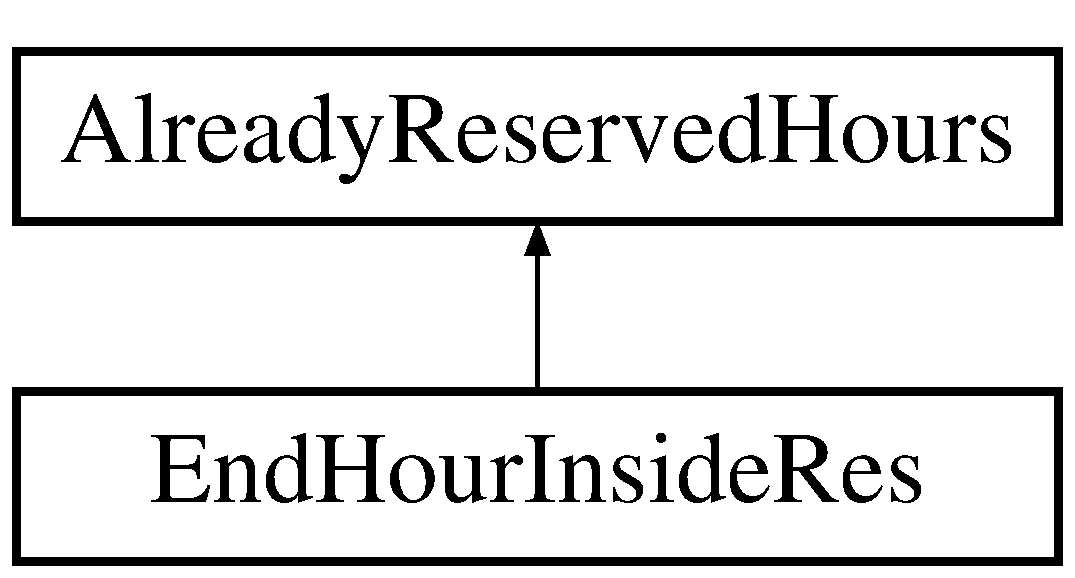
\includegraphics[height=2.000000cm]{class_end_hour_inside_res}
\end{center}
\end{figure}
\subsection*{Public Member Functions}
\begin{DoxyCompactItemize}
\item 
\mbox{\Hypertarget{class_end_hour_inside_res_af2162a2e870bf25d64f773089def5ec2}\label{class_end_hour_inside_res_af2162a2e870bf25d64f773089def5ec2}} 
{\bfseries End\+Hour\+Inside\+Res} (double res\+Start, double res\+End)
\item 
\mbox{\Hypertarget{class_end_hour_inside_res_afee9514b15c167847bc55ebe833076ff}\label{class_end_hour_inside_res_afee9514b15c167847bc55ebe833076ff}} 
std\+::string {\bfseries what} () const
\end{DoxyCompactItemize}


The documentation for this class was generated from the following files\+:\begin{DoxyCompactItemize}
\item 
Person.\+h\item 
Person.\+cpp\end{DoxyCompactItemize}

\hypertarget{class_free}{}\section{Free Class Reference}
\label{class_free}\index{Free@{Free}}
Inheritance diagram for Free\+:\begin{figure}[H]
\begin{center}
\leavevmode
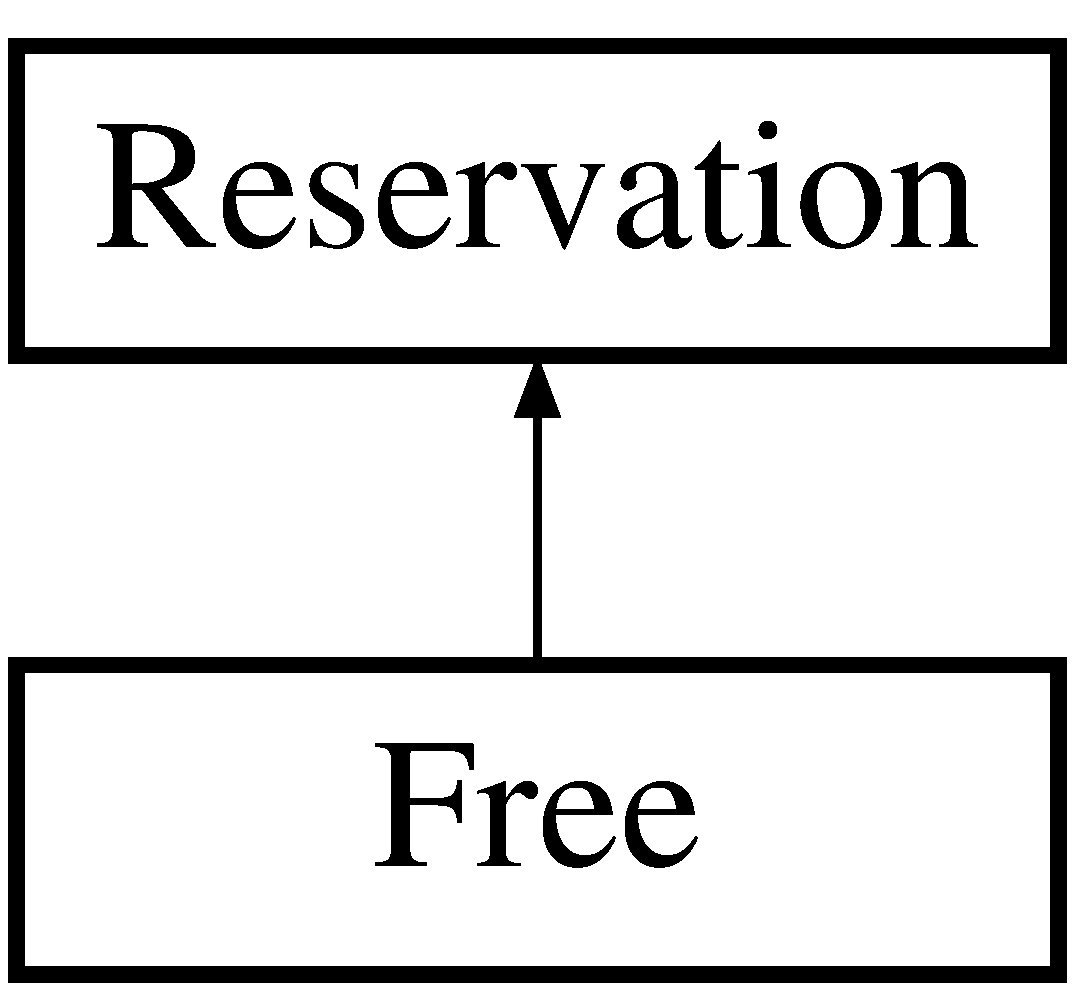
\includegraphics[height=2.000000cm]{class_free}
\end{center}
\end{figure}
\subsection*{Public Member Functions}
\begin{DoxyCompactItemize}
\item 
\mbox{\Hypertarget{class_free_a4a847fee0a934284fc4581282706e885}\label{class_free_a4a847fee0a934284fc4581282706e885}} 
\mbox{\hyperlink{class_free_a4a847fee0a934284fc4581282706e885}{Free}} ()
\begin{DoxyCompactList}\small\item\em Constructor of Class. \end{DoxyCompactList}\item 
\mbox{\hyperlink{class_free_afe1bb925d237595d9fd75fb2e7772314}{Free}} (int m, int d, double str\+Hr, double p, unsigned int dur)
\item 
double \mbox{\hyperlink{class_free_a229f009a7535eeba0a6ff4495de8c6bf}{get\+Price}} ()
\begin{DoxyCompactList}\small\item\em Method to obtain the price of the free. \end{DoxyCompactList}\item 
void \mbox{\hyperlink{class_free_a5eec9da16ebf4f388d16dd270bd93b64}{store\+Info}} (std\+::ofstream \&outfile, int \mbox{\hyperlink{class_reservation_a480981ed050bae19bc74bbb0bbb459f9}{indent}})
\begin{DoxyCompactList}\small\item\em Store in the information of the \mbox{\hyperlink{class_free}{Free}} to a file. \end{DoxyCompactList}\item 
void \mbox{\hyperlink{class_free_ad1023c825c9790edf0797e2e69dd2fcf}{read\+Info}} (std\+::ifstream \&infile)
\begin{DoxyCompactList}\small\item\em Reading the information of a \mbox{\hyperlink{class_free}{Free}} from a file. \end{DoxyCompactList}\end{DoxyCompactItemize}
\subsection*{Additional Inherited Members}


\subsection{Constructor \& Destructor Documentation}
\mbox{\Hypertarget{class_free_afe1bb925d237595d9fd75fb2e7772314}\label{class_free_afe1bb925d237595d9fd75fb2e7772314}} 
\index{Free@{Free}!Free@{Free}}
\index{Free@{Free}!Free@{Free}}
\subsubsection{\texorpdfstring{Free()}{Free()}}
{\footnotesize\ttfamily Free\+::\+Free (\begin{DoxyParamCaption}\item[{int}]{m,  }\item[{int}]{d,  }\item[{double}]{str\+Hr,  }\item[{double}]{p,  }\item[{unsigned int}]{dur }\end{DoxyParamCaption})}

Constructor of Class 
\begin{DoxyParams}{Parameters}
{\em m} & -\/ month of the reservation \\
\hline
{\em d} & -\/ day of the reservation \\
\hline
{\em str\+Hr} & -\/ starting Hour of the reservation \\
\hline
{\em p} & -\/ price of the reservation \\
\hline
{\em dur} & -\/ duration of the reservation \\
\hline
\end{DoxyParams}


\subsection{Member Function Documentation}
\mbox{\Hypertarget{class_free_a229f009a7535eeba0a6ff4495de8c6bf}\label{class_free_a229f009a7535eeba0a6ff4495de8c6bf}} 
\index{Free@{Free}!get\+Price@{get\+Price}}
\index{get\+Price@{get\+Price}!Free@{Free}}
\subsubsection{\texorpdfstring{get\+Price()}{getPrice()}}
{\footnotesize\ttfamily double Free\+::get\+Price (\begin{DoxyParamCaption}{ }\end{DoxyParamCaption})\hspace{0.3cm}{\ttfamily [virtual]}}



Method to obtain the price of the free. 

\begin{DoxyReturn}{Returns}
Price of the lesson 
\end{DoxyReturn}


Reimplemented from \mbox{\hyperlink{class_reservation_a62cdb2f1a24e2fce92fb9f024ae9f494}{Reservation}}.

\mbox{\Hypertarget{class_free_ad1023c825c9790edf0797e2e69dd2fcf}\label{class_free_ad1023c825c9790edf0797e2e69dd2fcf}} 
\index{Free@{Free}!read\+Info@{read\+Info}}
\index{read\+Info@{read\+Info}!Free@{Free}}
\subsubsection{\texorpdfstring{read\+Info()}{readInfo()}}
{\footnotesize\ttfamily void Free\+::read\+Info (\begin{DoxyParamCaption}\item[{std\+::ifstream \&}]{infile }\end{DoxyParamCaption})\hspace{0.3cm}{\ttfamily [virtual]}}



Reading the information of a \mbox{\hyperlink{class_free}{Free}} from a file. 


\begin{DoxyParams}{Parameters}
{\em infile} & -\/ file to read the information from \\
\hline
\end{DoxyParams}


Reimplemented from \mbox{\hyperlink{class_reservation_acff32024a350c2156af9f74522c59b7b}{Reservation}}.

\mbox{\Hypertarget{class_free_a5eec9da16ebf4f388d16dd270bd93b64}\label{class_free_a5eec9da16ebf4f388d16dd270bd93b64}} 
\index{Free@{Free}!store\+Info@{store\+Info}}
\index{store\+Info@{store\+Info}!Free@{Free}}
\subsubsection{\texorpdfstring{store\+Info()}{storeInfo()}}
{\footnotesize\ttfamily void Free\+::store\+Info (\begin{DoxyParamCaption}\item[{std\+::ofstream \&}]{outfile,  }\item[{int}]{indent }\end{DoxyParamCaption})\hspace{0.3cm}{\ttfamily [virtual]}}



Store in the information of the \mbox{\hyperlink{class_free}{Free}} to a file. 


\begin{DoxyParams}{Parameters}
{\em outfile} & -\/ the file to write information \\
\hline
{\em indent} & -\/ current indentation \\
\hline
\end{DoxyParams}


Reimplemented from \mbox{\hyperlink{class_reservation_a8ec83fe2eb15294c3a51a9998ed17df7}{Reservation}}.



The documentation for this class was generated from the following files\+:\begin{DoxyCompactItemize}
\item 
Reservation.\+h\item 
Reservation.\+cpp\end{DoxyCompactItemize}

\hypertarget{class_incorrect_month}{}\section{Incorrect\+Month Class Reference}
\label{class_incorrect_month}\index{Incorrect\+Month@{Incorrect\+Month}}


{\ttfamily \#include $<$Person.\+h$>$}

\subsection*{Public Member Functions}
\begin{DoxyCompactItemize}
\item 
\mbox{\Hypertarget{class_incorrect_month_ab5f69a2380802c07d44f2f1c5e6575ed}\label{class_incorrect_month_ab5f69a2380802c07d44f2f1c5e6575ed}} 
std\+::string {\bfseries what} () const
\end{DoxyCompactItemize}


\subsection{Detailed Description}
When the month does not exist 

The documentation for this class was generated from the following files\+:\begin{DoxyCompactItemize}
\item 
Person.\+h\item 
Person.\+cpp\end{DoxyCompactItemize}

\hypertarget{class_inside_res}{}\section{Inside\+Res Class Reference}
\label{class_inside_res}\index{Inside\+Res@{Inside\+Res}}
Inheritance diagram for Inside\+Res\+:\begin{figure}[H]
\begin{center}
\leavevmode
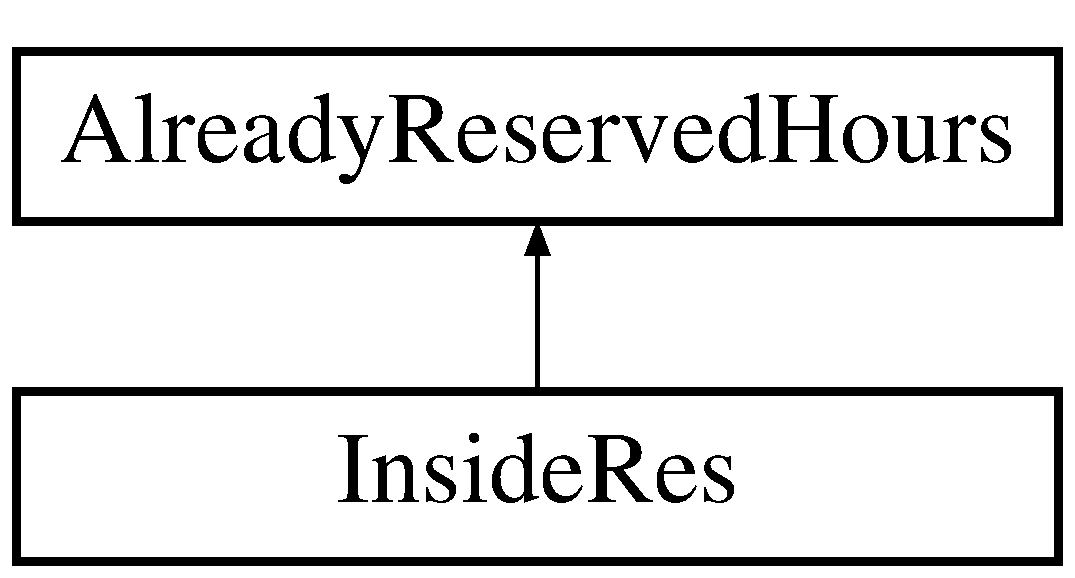
\includegraphics[height=2.000000cm]{class_inside_res}
\end{center}
\end{figure}
\subsection*{Public Member Functions}
\begin{DoxyCompactItemize}
\item 
\mbox{\Hypertarget{class_inside_res_ad447dd2fb8257c0e07ff171b6b8403d9}\label{class_inside_res_ad447dd2fb8257c0e07ff171b6b8403d9}} 
{\bfseries Inside\+Res} (double res\+Start, double end\+Hour)
\item 
\mbox{\Hypertarget{class_inside_res_af8e96688976739ec91630a369d4b94e7}\label{class_inside_res_af8e96688976739ec91630a369d4b94e7}} 
std\+::string {\bfseries what} () const
\end{DoxyCompactItemize}


The documentation for this class was generated from the following files\+:\begin{DoxyCompactItemize}
\item 
Person.\+h\item 
Person.\+cpp\end{DoxyCompactItemize}

\hypertarget{class_invalid_age}{}\section{Invalid\+Age Class Reference}
\label{class_invalid_age}\index{Invalid\+Age@{Invalid\+Age}}


{\ttfamily \#include $<$Company.\+h$>$}

\subsection*{Public Member Functions}
\begin{DoxyCompactItemize}
\item 
\mbox{\hyperlink{class_invalid_age_ae1ed3ee78dd4c589a64d939b90aa09f3}{Invalid\+Age}} (int age)
\item 
std\+::string \mbox{\hyperlink{class_invalid_age_a6961abe914f41e975a7b0ebd526e3ea4}{what}} () const
\end{DoxyCompactItemize}


\subsection{Detailed Description}
When the age is not valid 

\subsection{Constructor \& Destructor Documentation}
\mbox{\Hypertarget{class_invalid_age_ae1ed3ee78dd4c589a64d939b90aa09f3}\label{class_invalid_age_ae1ed3ee78dd4c589a64d939b90aa09f3}} 
\index{Invalid\+Age@{Invalid\+Age}!Invalid\+Age@{Invalid\+Age}}
\index{Invalid\+Age@{Invalid\+Age}!Invalid\+Age@{Invalid\+Age}}
\subsubsection{\texorpdfstring{Invalid\+Age()}{InvalidAge()}}
{\footnotesize\ttfamily Invalid\+Age\+::\+Invalid\+Age (\begin{DoxyParamCaption}\item[{int}]{age }\end{DoxyParamCaption})\hspace{0.3cm}{\ttfamily [inline]}}



\subsection{Member Function Documentation}
\mbox{\Hypertarget{class_invalid_age_a6961abe914f41e975a7b0ebd526e3ea4}\label{class_invalid_age_a6961abe914f41e975a7b0ebd526e3ea4}} 
\index{Invalid\+Age@{Invalid\+Age}!what@{what}}
\index{what@{what}!Invalid\+Age@{Invalid\+Age}}
\subsubsection{\texorpdfstring{what()}{what()}}
{\footnotesize\ttfamily string Invalid\+Age\+::what (\begin{DoxyParamCaption}{ }\end{DoxyParamCaption}) const}



The documentation for this class was generated from the following files\+:\begin{DoxyCompactItemize}
\item 
\mbox{\hyperlink{_company_8h}{Company.\+h}}\item 
\mbox{\hyperlink{_company_8cpp}{Company.\+cpp}}\end{DoxyCompactItemize}

\hypertarget{class_invalid_date}{}\section{Invalid\+Date Class Reference}
\label{class_invalid_date}\index{Invalid\+Date@{Invalid\+Date}}
\subsection*{Public Member Functions}
\begin{DoxyCompactItemize}
\item 
\mbox{\Hypertarget{class_invalid_date_a0a8dd2b0c6857849e97680df8d99952d}\label{class_invalid_date_a0a8dd2b0c6857849e97680df8d99952d}} 
{\bfseries Invalid\+Date} (int day, int month)
\item 
\mbox{\Hypertarget{class_invalid_date_aa27c136303d6b0b0184eb0abf3ef78e3}\label{class_invalid_date_aa27c136303d6b0b0184eb0abf3ef78e3}} 
std\+::string {\bfseries what} () const
\end{DoxyCompactItemize}


The documentation for this class was generated from the following files\+:\begin{DoxyCompactItemize}
\item 
Company.\+h\item 
Company.\+cpp\end{DoxyCompactItemize}

\hypertarget{class_invalid_grade}{}\section{Invalid\+Grade Class Reference}
\label{class_invalid_grade}\index{Invalid\+Grade@{Invalid\+Grade}}


{\ttfamily \#include $<$Report.\+h$>$}

\subsection*{Public Member Functions}
\begin{DoxyCompactItemize}
\item 
\mbox{\Hypertarget{class_invalid_grade_a45b993c52fbd0083f8344a4e437b0fd8}\label{class_invalid_grade_a45b993c52fbd0083f8344a4e437b0fd8}} 
{\bfseries Invalid\+Grade} (int grade)
\item 
\mbox{\Hypertarget{class_invalid_grade_a804b310f3aa6d5b388ff36dac76b06da}\label{class_invalid_grade_a804b310f3aa6d5b388ff36dac76b06da}} 
int {\bfseries get\+Grade} () const
\end{DoxyCompactItemize}
\subsection*{Friends}
\begin{DoxyCompactItemize}
\item 
\mbox{\Hypertarget{class_invalid_grade_abd6d4b28be315c2b68592594412c7632}\label{class_invalid_grade_abd6d4b28be315c2b68592594412c7632}} 
std\+::ostream \& {\bfseries operator$<$$<$} (std\+::ostream \&os, const \mbox{\hyperlink{class_invalid_grade}{Invalid\+Grade}} \&ig)
\end{DoxyCompactItemize}


\subsection{Detailed Description}
When the grade is not valid 

The documentation for this class was generated from the following file\+:\begin{DoxyCompactItemize}
\item 
Report.\+h\end{DoxyCompactItemize}

\hypertarget{class_invoice}{}\section{Invoice Class Reference}
\label{class_invoice}\index{Invoice@{Invoice}}


{\ttfamily \#include $<$Invoice.\+h$>$}

\subsection*{Public Member Functions}
\begin{DoxyCompactItemize}
\item 
\mbox{\Hypertarget{class_invoice_a25d6ad261479340ac3775e21f03eef90}\label{class_invoice_a25d6ad261479340ac3775e21f03eef90}} 
\mbox{\hyperlink{class_invoice_a25d6ad261479340ac3775e21f03eef90}{Invoice}} ()
\begin{DoxyCompactList}\small\item\em Class Constructor. \end{DoxyCompactList}\item 
\mbox{\hyperlink{class_invoice_a332d51ff2cf16d52178fa61ddc69f017}{Invoice}} (std\+::string name, std\+::string teacher\+Name, std\+::vector$<$ \mbox{\hyperlink{class_reservation}{Reservation}} $\ast$$>$ reservs)
\begin{DoxyCompactList}\small\item\em Class Constructor. \end{DoxyCompactList}\item 
double \mbox{\hyperlink{class_invoice_a049d93832eedd6c40a0b5a686771bdb6}{get\+Price}} () const
\begin{DoxyCompactList}\small\item\em Getter of the price of the month. \end{DoxyCompactList}\item 
std\+::vector$<$ \mbox{\hyperlink{class_reservation}{Reservation}} $\ast$ $>$ \mbox{\hyperlink{class_invoice_a98ede540a39d22c91a3bc6c5b28116fd}{get\+Reservs}} ()
\begin{DoxyCompactList}\small\item\em Getter of the reservations. \end{DoxyCompactList}\item 
void \mbox{\hyperlink{class_invoice_a326f9548d517f1f432939e0c8231a84e}{store\+Info}} (std\+::ofstream \&outfile, int indent)
\begin{DoxyCompactList}\small\item\em Store in the information of the \mbox{\hyperlink{class_court}{Court}} to a file. \end{DoxyCompactList}\item 
void \mbox{\hyperlink{class_invoice_a08ce5090cf11e9f74820810d3796dea2}{indentation}} (std\+::ofstream \&outfile, int indent)
\begin{DoxyCompactList}\small\item\em Indenting the file. \end{DoxyCompactList}\item 
void \mbox{\hyperlink{class_invoice_aae19e485510f08c56be425b4634246ed}{read\+Info}} (std\+::ifstream \&infile)
\begin{DoxyCompactList}\small\item\em Reading the information of a \mbox{\hyperlink{class_date}{Date}} from a file. \end{DoxyCompactList}\end{DoxyCompactItemize}
\subsection*{Friends}
\begin{DoxyCompactItemize}
\item 
std\+::ostream \& \mbox{\hyperlink{class_invoice_a1ff3da2cc7abd9df37b2936772ce9ff7}{operator$<$$<$}} (std\+::ostream \&out, \mbox{\hyperlink{class_invoice}{Invoice}} inv)
\begin{DoxyCompactList}\small\item\em Writer of the invoice to the screen. \end{DoxyCompactList}\end{DoxyCompactItemize}


\subsection{Detailed Description}
\mbox{\hyperlink{class_invoice}{Invoice}} of the month for the user 

\subsection{Constructor \& Destructor Documentation}
\mbox{\Hypertarget{class_invoice_a332d51ff2cf16d52178fa61ddc69f017}\label{class_invoice_a332d51ff2cf16d52178fa61ddc69f017}} 
\index{Invoice@{Invoice}!Invoice@{Invoice}}
\index{Invoice@{Invoice}!Invoice@{Invoice}}
\subsubsection{\texorpdfstring{Invoice()}{Invoice()}}
{\footnotesize\ttfamily Invoice\+::\+Invoice (\begin{DoxyParamCaption}\item[{std\+::string}]{name,  }\item[{std\+::string}]{teacher\+Name,  }\item[{std\+::vector$<$ \mbox{\hyperlink{class_reservation}{Reservation}} $\ast$$>$}]{reservs }\end{DoxyParamCaption})}



Class Constructor. 


\begin{DoxyParams}{Parameters}
{\em name} & -\/ name of \mbox{\hyperlink{class_user}{User}} \\
\hline
{\em teacher\+Name} & -\/ name of \mbox{\hyperlink{class_teacher}{Teacher}} \\
\hline
{\em reservs} & -\/ The reservations \\
\hline
\end{DoxyParams}


\subsection{Member Function Documentation}
\mbox{\Hypertarget{class_invoice_a049d93832eedd6c40a0b5a686771bdb6}\label{class_invoice_a049d93832eedd6c40a0b5a686771bdb6}} 
\index{Invoice@{Invoice}!get\+Price@{get\+Price}}
\index{get\+Price@{get\+Price}!Invoice@{Invoice}}
\subsubsection{\texorpdfstring{get\+Price()}{getPrice()}}
{\footnotesize\ttfamily double Invoice\+::get\+Price (\begin{DoxyParamCaption}{ }\end{DoxyParamCaption}) const}



Getter of the price of the month. 

\begin{DoxyReturn}{Returns}
the price to pay 
\end{DoxyReturn}
\mbox{\Hypertarget{class_invoice_a98ede540a39d22c91a3bc6c5b28116fd}\label{class_invoice_a98ede540a39d22c91a3bc6c5b28116fd}} 
\index{Invoice@{Invoice}!get\+Reservs@{get\+Reservs}}
\index{get\+Reservs@{get\+Reservs}!Invoice@{Invoice}}
\subsubsection{\texorpdfstring{get\+Reservs()}{getReservs()}}
{\footnotesize\ttfamily vector$<$ \mbox{\hyperlink{class_reservation}{Reservation}} $\ast$ $>$ Invoice\+::get\+Reservs (\begin{DoxyParamCaption}{ }\end{DoxyParamCaption})}



Getter of the reservations. 

\begin{DoxyReturn}{Returns}
vector of reservations 
\end{DoxyReturn}
\mbox{\Hypertarget{class_invoice_a08ce5090cf11e9f74820810d3796dea2}\label{class_invoice_a08ce5090cf11e9f74820810d3796dea2}} 
\index{Invoice@{Invoice}!indentation@{indentation}}
\index{indentation@{indentation}!Invoice@{Invoice}}
\subsubsection{\texorpdfstring{indentation()}{indentation()}}
{\footnotesize\ttfamily void Invoice\+::indentation (\begin{DoxyParamCaption}\item[{std\+::ofstream \&}]{outfile,  }\item[{int}]{indent }\end{DoxyParamCaption})}



Indenting the file. 


\begin{DoxyParams}{Parameters}
{\em outfile} & -\/ the file to write information \\
\hline
{\em indent} & -\/ current indentation \\
\hline
\end{DoxyParams}
\mbox{\Hypertarget{class_invoice_aae19e485510f08c56be425b4634246ed}\label{class_invoice_aae19e485510f08c56be425b4634246ed}} 
\index{Invoice@{Invoice}!read\+Info@{read\+Info}}
\index{read\+Info@{read\+Info}!Invoice@{Invoice}}
\subsubsection{\texorpdfstring{read\+Info()}{readInfo()}}
{\footnotesize\ttfamily void Invoice\+::read\+Info (\begin{DoxyParamCaption}\item[{std\+::ifstream \&}]{infile }\end{DoxyParamCaption})}



Reading the information of a \mbox{\hyperlink{class_date}{Date}} from a file. 


\begin{DoxyParams}{Parameters}
{\em infile} & -\/ file to read the information from \\
\hline
\end{DoxyParams}
\mbox{\Hypertarget{class_invoice_a326f9548d517f1f432939e0c8231a84e}\label{class_invoice_a326f9548d517f1f432939e0c8231a84e}} 
\index{Invoice@{Invoice}!store\+Info@{store\+Info}}
\index{store\+Info@{store\+Info}!Invoice@{Invoice}}
\subsubsection{\texorpdfstring{store\+Info()}{storeInfo()}}
{\footnotesize\ttfamily void Invoice\+::store\+Info (\begin{DoxyParamCaption}\item[{std\+::ofstream \&}]{outfile,  }\item[{int}]{indent }\end{DoxyParamCaption})}



Store in the information of the \mbox{\hyperlink{class_court}{Court}} to a file. 


\begin{DoxyParams}{Parameters}
{\em outfile} & -\/ the file to write information \\
\hline
{\em indent} & -\/ current indentation \\
\hline
\end{DoxyParams}


\subsection{Friends And Related Function Documentation}
\mbox{\Hypertarget{class_invoice_a1ff3da2cc7abd9df37b2936772ce9ff7}\label{class_invoice_a1ff3da2cc7abd9df37b2936772ce9ff7}} 
\index{Invoice@{Invoice}!operator$<$$<$@{operator$<$$<$}}
\index{operator$<$$<$@{operator$<$$<$}!Invoice@{Invoice}}
\subsubsection{\texorpdfstring{operator$<$$<$}{operator<<}}
{\footnotesize\ttfamily std\+::ostream\& operator$<$$<$ (\begin{DoxyParamCaption}\item[{std\+::ostream \&}]{out,  }\item[{\mbox{\hyperlink{class_invoice}{Invoice}}}]{inv }\end{DoxyParamCaption})\hspace{0.3cm}{\ttfamily [friend]}}



Writer of the invoice to the screen. 


\begin{DoxyParams}{Parameters}
{\em out} & -\/ where to write it to \\
\hline
{\em inv} & -\/ The actual invoice \\
\hline
\end{DoxyParams}
\begin{DoxyReturn}{Returns}
the stream itself 
\end{DoxyReturn}


The documentation for this class was generated from the following files\+:\begin{DoxyCompactItemize}
\item 
Invoice.\+h\item 
Invoice.\+cpp\end{DoxyCompactItemize}

\hypertarget{class_invoice_already_exists}{}\section{Invoice\+Already\+Exists Class Reference}
\label{class_invoice_already_exists}\index{Invoice\+Already\+Exists@{Invoice\+Already\+Exists}}


{\ttfamily \#include $<$Person.\+h$>$}

\subsection*{Public Member Functions}
\begin{DoxyCompactItemize}
\item 
\mbox{\hyperlink{class_invoice_already_exists_ae5d642f496997633c4a4dbc3c8347374}{Invoice\+Already\+Exists}} (int month)
\item 
int \mbox{\hyperlink{class_invoice_already_exists_a75da257c1dfbaa7cacf89e79c759eb43}{get\+Month}} ()
\item 
std\+::string \mbox{\hyperlink{class_invoice_already_exists_ae0239e7ba5445491a3182d77d34b1505}{what}} () const
\end{DoxyCompactItemize}


\subsection{Constructor \& Destructor Documentation}
\mbox{\Hypertarget{class_invoice_already_exists_ae5d642f496997633c4a4dbc3c8347374}\label{class_invoice_already_exists_ae5d642f496997633c4a4dbc3c8347374}} 
\index{Invoice\+Already\+Exists@{Invoice\+Already\+Exists}!Invoice\+Already\+Exists@{Invoice\+Already\+Exists}}
\index{Invoice\+Already\+Exists@{Invoice\+Already\+Exists}!Invoice\+Already\+Exists@{Invoice\+Already\+Exists}}
\subsubsection{\texorpdfstring{Invoice\+Already\+Exists()}{InvoiceAlreadyExists()}}
{\footnotesize\ttfamily Invoice\+Already\+Exists\+::\+Invoice\+Already\+Exists (\begin{DoxyParamCaption}\item[{int}]{month }\end{DoxyParamCaption})\hspace{0.3cm}{\ttfamily [inline]}}



\subsection{Member Function Documentation}
\mbox{\Hypertarget{class_invoice_already_exists_a75da257c1dfbaa7cacf89e79c759eb43}\label{class_invoice_already_exists_a75da257c1dfbaa7cacf89e79c759eb43}} 
\index{Invoice\+Already\+Exists@{Invoice\+Already\+Exists}!get\+Month@{get\+Month}}
\index{get\+Month@{get\+Month}!Invoice\+Already\+Exists@{Invoice\+Already\+Exists}}
\subsubsection{\texorpdfstring{get\+Month()}{getMonth()}}
{\footnotesize\ttfamily int Invoice\+Already\+Exists\+::get\+Month (\begin{DoxyParamCaption}{ }\end{DoxyParamCaption})\hspace{0.3cm}{\ttfamily [inline]}}

\mbox{\Hypertarget{class_invoice_already_exists_ae0239e7ba5445491a3182d77d34b1505}\label{class_invoice_already_exists_ae0239e7ba5445491a3182d77d34b1505}} 
\index{Invoice\+Already\+Exists@{Invoice\+Already\+Exists}!what@{what}}
\index{what@{what}!Invoice\+Already\+Exists@{Invoice\+Already\+Exists}}
\subsubsection{\texorpdfstring{what()}{what()}}
{\footnotesize\ttfamily string Invoice\+Already\+Exists\+::what (\begin{DoxyParamCaption}{ }\end{DoxyParamCaption}) const}



The documentation for this class was generated from the following files\+:\begin{DoxyCompactItemize}
\item 
\mbox{\hyperlink{_person_8h}{Person.\+h}}\item 
\mbox{\hyperlink{_person_8cpp}{Person.\+cpp}}\end{DoxyCompactItemize}

\hypertarget{class_invoice_not_available}{}\section{Invoice\+Not\+Available Class Reference}
\label{class_invoice_not_available}\index{Invoice\+Not\+Available@{Invoice\+Not\+Available}}


{\ttfamily \#include $<$Person.\+h$>$}

\subsection*{Public Member Functions}
\begin{DoxyCompactItemize}
\item 
\mbox{\hyperlink{class_invoice_not_available_ad8821a4be3e8d48aef9dcd971cc9e0d0}{Invoice\+Not\+Available}} (int \mbox{\hyperlink{class_invoice_not_available_a35029f0aa54b16c927f45adbac81f427}{month}})
\item 
int \mbox{\hyperlink{class_invoice_not_available_aba76622dae4202950c43956f6ed0930e}{get\+Month}} ()
\item 
std\+::string \mbox{\hyperlink{class_invoice_not_available_a77e49a07e8605a37f1a4c6c59742b898}{what}} () const
\end{DoxyCompactItemize}
\subsection*{Public Attributes}
\begin{DoxyCompactItemize}
\item 
int \mbox{\hyperlink{class_invoice_not_available_a35029f0aa54b16c927f45adbac81f427}{month}}
\end{DoxyCompactItemize}


\subsection{Constructor \& Destructor Documentation}
\mbox{\Hypertarget{class_invoice_not_available_ad8821a4be3e8d48aef9dcd971cc9e0d0}\label{class_invoice_not_available_ad8821a4be3e8d48aef9dcd971cc9e0d0}} 
\index{Invoice\+Not\+Available@{Invoice\+Not\+Available}!Invoice\+Not\+Available@{Invoice\+Not\+Available}}
\index{Invoice\+Not\+Available@{Invoice\+Not\+Available}!Invoice\+Not\+Available@{Invoice\+Not\+Available}}
\subsubsection{\texorpdfstring{Invoice\+Not\+Available()}{InvoiceNotAvailable()}}
{\footnotesize\ttfamily Invoice\+Not\+Available\+::\+Invoice\+Not\+Available (\begin{DoxyParamCaption}\item[{int}]{month }\end{DoxyParamCaption})\hspace{0.3cm}{\ttfamily [inline]}}



\subsection{Member Function Documentation}
\mbox{\Hypertarget{class_invoice_not_available_aba76622dae4202950c43956f6ed0930e}\label{class_invoice_not_available_aba76622dae4202950c43956f6ed0930e}} 
\index{Invoice\+Not\+Available@{Invoice\+Not\+Available}!get\+Month@{get\+Month}}
\index{get\+Month@{get\+Month}!Invoice\+Not\+Available@{Invoice\+Not\+Available}}
\subsubsection{\texorpdfstring{get\+Month()}{getMonth()}}
{\footnotesize\ttfamily int Invoice\+Not\+Available\+::get\+Month (\begin{DoxyParamCaption}{ }\end{DoxyParamCaption})\hspace{0.3cm}{\ttfamily [inline]}}

\mbox{\Hypertarget{class_invoice_not_available_a77e49a07e8605a37f1a4c6c59742b898}\label{class_invoice_not_available_a77e49a07e8605a37f1a4c6c59742b898}} 
\index{Invoice\+Not\+Available@{Invoice\+Not\+Available}!what@{what}}
\index{what@{what}!Invoice\+Not\+Available@{Invoice\+Not\+Available}}
\subsubsection{\texorpdfstring{what()}{what()}}
{\footnotesize\ttfamily string Invoice\+Not\+Available\+::what (\begin{DoxyParamCaption}{ }\end{DoxyParamCaption}) const}



\subsection{Member Data Documentation}
\mbox{\Hypertarget{class_invoice_not_available_a35029f0aa54b16c927f45adbac81f427}\label{class_invoice_not_available_a35029f0aa54b16c927f45adbac81f427}} 
\index{Invoice\+Not\+Available@{Invoice\+Not\+Available}!month@{month}}
\index{month@{month}!Invoice\+Not\+Available@{Invoice\+Not\+Available}}
\subsubsection{\texorpdfstring{month}{month}}
{\footnotesize\ttfamily int Invoice\+Not\+Available\+::month}



The documentation for this class was generated from the following files\+:\begin{DoxyCompactItemize}
\item 
\mbox{\hyperlink{_person_8h}{Person.\+h}}\item 
\mbox{\hyperlink{_person_8cpp}{Person.\+cpp}}\end{DoxyCompactItemize}

\hypertarget{class_lesson}{}\section{Lesson Class Reference}
\label{class_lesson}\index{Lesson@{Lesson}}


{\ttfamily \#include $<$Reservation.\+h$>$}

Inheritance diagram for Lesson\+:\begin{figure}[H]
\begin{center}
\leavevmode
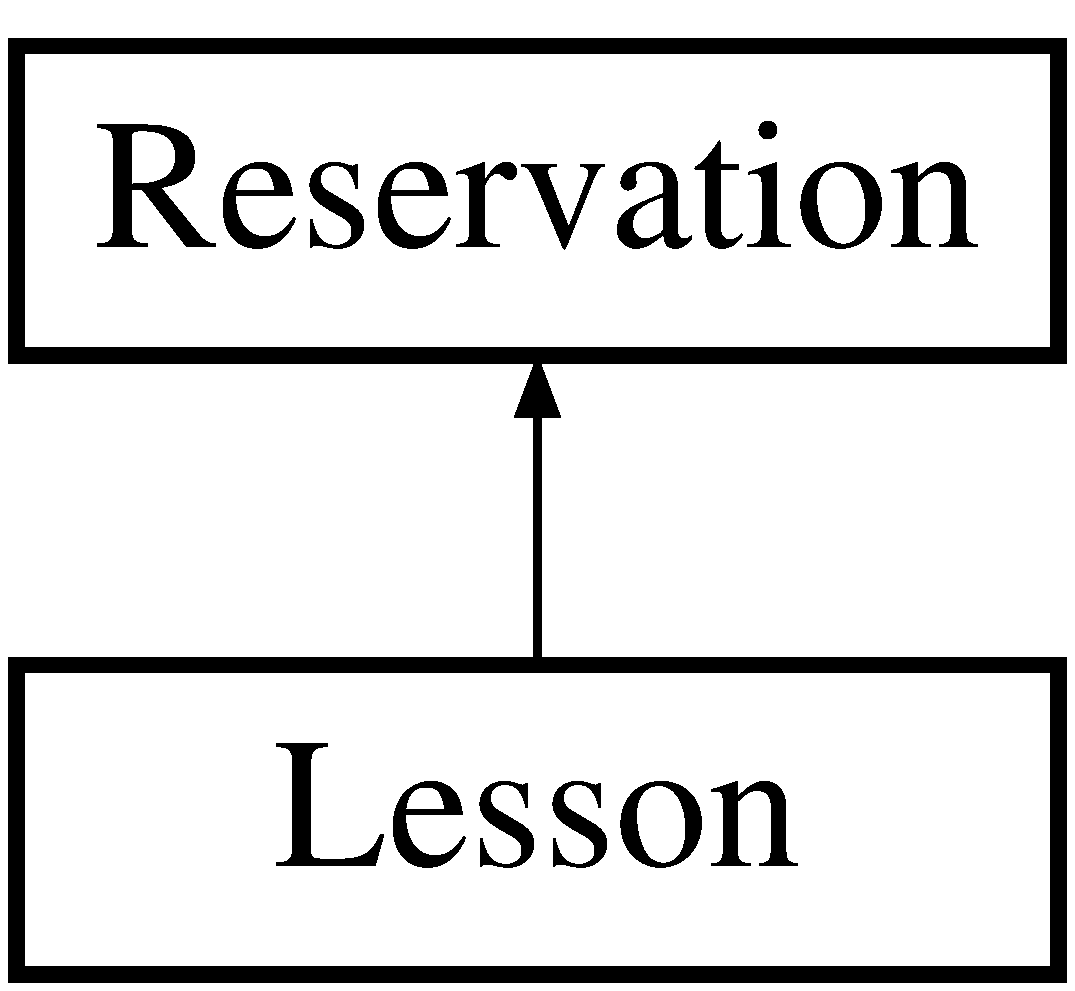
\includegraphics[height=2.000000cm]{class_lesson}
\end{center}
\end{figure}
\subsection*{Public Member Functions}
\begin{DoxyCompactItemize}
\item 
\mbox{\Hypertarget{class_lesson_a1f6ed0da97171480b7d6d5696d6f2afc}\label{class_lesson_a1f6ed0da97171480b7d6d5696d6f2afc}} 
\mbox{\hyperlink{class_lesson_a1f6ed0da97171480b7d6d5696d6f2afc}{Lesson}} ()
\begin{DoxyCompactList}\small\item\em Constructor of a lesson. \end{DoxyCompactList}\item 
\mbox{\hyperlink{class_lesson_a2d02413d32e4df560bcdb8cc9d00f7d7}{Lesson}} (int m, int d, int str\+Hr, double \mbox{\hyperlink{class_reservation_a82e197bd30e7949ee9b8616ee4eacf83}{price}}, unsigned int dr)
\begin{DoxyCompactList}\small\item\em Constructor of a lesson. \end{DoxyCompactList}\item 
double \mbox{\hyperlink{class_lesson_ad7a2f708f870040627a442cdf000683f}{get\+Price}} ()
\begin{DoxyCompactList}\small\item\em Method to obtain the price of the lesson. \end{DoxyCompactList}\item 
void \mbox{\hyperlink{class_lesson_a645855060ab3c915a6e0875bc5584887}{store\+Info}} (std\+::ofstream \&outfile, int \mbox{\hyperlink{class_reservation_a480981ed050bae19bc74bbb0bbb459f9}{indent}})
\begin{DoxyCompactList}\small\item\em Store in the information of the lesson to a file. \end{DoxyCompactList}\item 
void \mbox{\hyperlink{class_lesson_a3ac64e2f79bc9e381634d5d30499e8f1}{read\+Info}} (std\+::ifstream \&infile)
\begin{DoxyCompactList}\small\item\em Reading the information of a lesson from a file. \end{DoxyCompactList}\end{DoxyCompactItemize}
\subsection*{Additional Inherited Members}


\subsection{Detailed Description}
A \mbox{\hyperlink{class_reservation}{Reservation}} with a \mbox{\hyperlink{class_teacher}{Teacher}} 

\subsection{Constructor \& Destructor Documentation}
\mbox{\Hypertarget{class_lesson_a2d02413d32e4df560bcdb8cc9d00f7d7}\label{class_lesson_a2d02413d32e4df560bcdb8cc9d00f7d7}} 
\index{Lesson@{Lesson}!Lesson@{Lesson}}
\index{Lesson@{Lesson}!Lesson@{Lesson}}
\subsubsection{\texorpdfstring{Lesson()}{Lesson()}}
{\footnotesize\ttfamily Lesson\+::\+Lesson (\begin{DoxyParamCaption}\item[{int}]{m,  }\item[{int}]{d,  }\item[{int}]{str\+Hr,  }\item[{double}]{price,  }\item[{unsigned int}]{dr }\end{DoxyParamCaption})}



Constructor of a lesson. 


\begin{DoxyParams}{Parameters}
{\em m} & -\/ \mbox{\hyperlink{class_month}{Month}} of the lesson \\
\hline
{\em d} & -\/ \mbox{\hyperlink{class_day}{Day}} of the lesson \\
\hline
{\em str\+Hr} & -\/ Starting Hour of the lesson \\
\hline
{\em price} & -\/ Price of the lesson \\
\hline
{\em dr} & -\/ Duration of the lesson \\
\hline
\end{DoxyParams}


\subsection{Member Function Documentation}
\mbox{\Hypertarget{class_lesson_ad7a2f708f870040627a442cdf000683f}\label{class_lesson_ad7a2f708f870040627a442cdf000683f}} 
\index{Lesson@{Lesson}!get\+Price@{get\+Price}}
\index{get\+Price@{get\+Price}!Lesson@{Lesson}}
\subsubsection{\texorpdfstring{get\+Price()}{getPrice()}}
{\footnotesize\ttfamily double Lesson\+::get\+Price (\begin{DoxyParamCaption}{ }\end{DoxyParamCaption})\hspace{0.3cm}{\ttfamily [virtual]}}



Method to obtain the price of the lesson. 

\begin{DoxyReturn}{Returns}
Price of the lesson 
\end{DoxyReturn}


Reimplemented from \mbox{\hyperlink{class_reservation_a62cdb2f1a24e2fce92fb9f024ae9f494}{Reservation}}.

\mbox{\Hypertarget{class_lesson_a3ac64e2f79bc9e381634d5d30499e8f1}\label{class_lesson_a3ac64e2f79bc9e381634d5d30499e8f1}} 
\index{Lesson@{Lesson}!read\+Info@{read\+Info}}
\index{read\+Info@{read\+Info}!Lesson@{Lesson}}
\subsubsection{\texorpdfstring{read\+Info()}{readInfo()}}
{\footnotesize\ttfamily void Lesson\+::read\+Info (\begin{DoxyParamCaption}\item[{std\+::ifstream \&}]{infile }\end{DoxyParamCaption})\hspace{0.3cm}{\ttfamily [virtual]}}



Reading the information of a lesson from a file. 


\begin{DoxyParams}{Parameters}
{\em infile} & -\/ file to read the information from \\
\hline
\end{DoxyParams}


Reimplemented from \mbox{\hyperlink{class_reservation_acff32024a350c2156af9f74522c59b7b}{Reservation}}.

\mbox{\Hypertarget{class_lesson_a645855060ab3c915a6e0875bc5584887}\label{class_lesson_a645855060ab3c915a6e0875bc5584887}} 
\index{Lesson@{Lesson}!store\+Info@{store\+Info}}
\index{store\+Info@{store\+Info}!Lesson@{Lesson}}
\subsubsection{\texorpdfstring{store\+Info()}{storeInfo()}}
{\footnotesize\ttfamily void Lesson\+::store\+Info (\begin{DoxyParamCaption}\item[{std\+::ofstream \&}]{outfile,  }\item[{int}]{indent }\end{DoxyParamCaption})\hspace{0.3cm}{\ttfamily [virtual]}}



Store in the information of the lesson to a file. 


\begin{DoxyParams}{Parameters}
{\em outfile} & -\/ the file to write information \\
\hline
{\em indent} & -\/ current indentation \\
\hline
\end{DoxyParams}


Reimplemented from \mbox{\hyperlink{class_reservation_a8ec83fe2eb15294c3a51a9998ed17df7}{Reservation}}.



The documentation for this class was generated from the following files\+:\begin{DoxyCompactItemize}
\item 
Reservation.\+h\item 
Reservation.\+cpp\end{DoxyCompactItemize}

\hypertarget{class_month}{}\section{Month Class Reference}
\label{class_month}\index{Month@{Month}}


{\ttfamily \#include $<$Calendar.\+h$>$}

\subsection*{Public Member Functions}
\begin{DoxyCompactItemize}
\item 
\mbox{\hyperlink{class_month_a36882c55ece9c4210ec1b01bd665ec89}{Month}} ()
\begin{DoxyCompactList}\small\item\em Class Constructor. \end{DoxyCompactList}\item 
\mbox{\hyperlink{class_month_a4abb71ddcd1dfed172a828d8598bbdc7}{Month}} (int month, int days)
\begin{DoxyCompactList}\small\item\em Class constructor. \end{DoxyCompactList}\item 
\mbox{\hyperlink{class_day}{Day}} \& \mbox{\hyperlink{class_month_aea6a1844798c684548c1de899cf620b2}{get\+Day}} (int day)
\item 
int \mbox{\hyperlink{class_month_a5bc7c527734f8bc303fea424cd265357}{get\+Month}} ()
\item 
int \mbox{\hyperlink{class_month_a901b9af10fe3f3dab931927c2ab77440}{get\+No\+Days}} ()
\begin{DoxyCompactList}\small\item\em Getter of the Number of days. \end{DoxyCompactList}\item 
void \mbox{\hyperlink{class_month_a816bb5d0a2d54283ece6924a7b54df36}{set\+Days}} (std\+::vector$<$ \mbox{\hyperlink{class_day}{Day}} $>$ days)
\begin{DoxyCompactList}\small\item\em Setter of the days. \end{DoxyCompactList}\item 
void \mbox{\hyperlink{class_month_a9f6e8f474768770ae897e53177eb1797}{set\+Month}} (int month)
\begin{DoxyCompactList}\small\item\em Setter of the month. \end{DoxyCompactList}\end{DoxyCompactItemize}


\subsection{Detailed Description}
The whole month of reservations 

\subsection{Constructor \& Destructor Documentation}
\mbox{\Hypertarget{class_month_a36882c55ece9c4210ec1b01bd665ec89}\label{class_month_a36882c55ece9c4210ec1b01bd665ec89}} 
\index{Month@{Month}!Month@{Month}}
\index{Month@{Month}!Month@{Month}}
\subsubsection{\texorpdfstring{Month()}{Month()}\hspace{0.1cm}{\footnotesize\ttfamily [1/2]}}
{\footnotesize\ttfamily Month\+::\+Month (\begin{DoxyParamCaption}{ }\end{DoxyParamCaption})\hspace{0.3cm}{\ttfamily [inline]}}



Class Constructor. 

\mbox{\Hypertarget{class_month_a4abb71ddcd1dfed172a828d8598bbdc7}\label{class_month_a4abb71ddcd1dfed172a828d8598bbdc7}} 
\index{Month@{Month}!Month@{Month}}
\index{Month@{Month}!Month@{Month}}
\subsubsection{\texorpdfstring{Month()}{Month()}\hspace{0.1cm}{\footnotesize\ttfamily [2/2]}}
{\footnotesize\ttfamily Month\+::\+Month (\begin{DoxyParamCaption}\item[{int}]{month,  }\item[{int}]{days }\end{DoxyParamCaption})}



Class constructor. 


\begin{DoxyParams}{Parameters}
{\em month} & -\/ the current month \\
\hline
{\em days} & -\/ number of days \\
\hline
\end{DoxyParams}


\subsection{Member Function Documentation}
\mbox{\Hypertarget{class_month_aea6a1844798c684548c1de899cf620b2}\label{class_month_aea6a1844798c684548c1de899cf620b2}} 
\index{Month@{Month}!get\+Day@{get\+Day}}
\index{get\+Day@{get\+Day}!Month@{Month}}
\subsubsection{\texorpdfstring{get\+Day()}{getDay()}}
{\footnotesize\ttfamily \mbox{\hyperlink{class_day}{Day}} \& Month\+::get\+Day (\begin{DoxyParamCaption}\item[{int}]{day }\end{DoxyParamCaption})}

Getter of the day 
\begin{DoxyParams}{Parameters}
{\em day} & -\/ the day wanted \\
\hline
\end{DoxyParams}
\begin{DoxyReturn}{Returns}
the day 
\end{DoxyReturn}
\mbox{\Hypertarget{class_month_a5bc7c527734f8bc303fea424cd265357}\label{class_month_a5bc7c527734f8bc303fea424cd265357}} 
\index{Month@{Month}!get\+Month@{get\+Month}}
\index{get\+Month@{get\+Month}!Month@{Month}}
\subsubsection{\texorpdfstring{get\+Month()}{getMonth()}}
{\footnotesize\ttfamily int Month\+::get\+Month (\begin{DoxyParamCaption}{ }\end{DoxyParamCaption})}

Getter of the month \begin{DoxyReturn}{Returns}
the month 
\end{DoxyReturn}
\mbox{\Hypertarget{class_month_a901b9af10fe3f3dab931927c2ab77440}\label{class_month_a901b9af10fe3f3dab931927c2ab77440}} 
\index{Month@{Month}!get\+No\+Days@{get\+No\+Days}}
\index{get\+No\+Days@{get\+No\+Days}!Month@{Month}}
\subsubsection{\texorpdfstring{get\+No\+Days()}{getNoDays()}}
{\footnotesize\ttfamily int Month\+::get\+No\+Days (\begin{DoxyParamCaption}{ }\end{DoxyParamCaption})}



Getter of the Number of days. 

\begin{DoxyReturn}{Returns}
number of days 
\end{DoxyReturn}
\mbox{\Hypertarget{class_month_a816bb5d0a2d54283ece6924a7b54df36}\label{class_month_a816bb5d0a2d54283ece6924a7b54df36}} 
\index{Month@{Month}!set\+Days@{set\+Days}}
\index{set\+Days@{set\+Days}!Month@{Month}}
\subsubsection{\texorpdfstring{set\+Days()}{setDays()}}
{\footnotesize\ttfamily void Month\+::set\+Days (\begin{DoxyParamCaption}\item[{std\+::vector$<$ \mbox{\hyperlink{class_day}{Day}} $>$}]{days }\end{DoxyParamCaption})}



Setter of the days. 


\begin{DoxyParams}{Parameters}
{\em days} & -\/ vector of days \\
\hline
\end{DoxyParams}
\mbox{\Hypertarget{class_month_a9f6e8f474768770ae897e53177eb1797}\label{class_month_a9f6e8f474768770ae897e53177eb1797}} 
\index{Month@{Month}!set\+Month@{set\+Month}}
\index{set\+Month@{set\+Month}!Month@{Month}}
\subsubsection{\texorpdfstring{set\+Month()}{setMonth()}}
{\footnotesize\ttfamily void Month\+::set\+Month (\begin{DoxyParamCaption}\item[{int}]{month }\end{DoxyParamCaption})}



Setter of the month. 


\begin{DoxyParams}{Parameters}
{\em month} & -\/ the month \\
\hline
\end{DoxyParams}


The documentation for this class was generated from the following files\+:\begin{DoxyCompactItemize}
\item 
\mbox{\hyperlink{_calendar_8h}{Calendar.\+h}}\item 
\mbox{\hyperlink{_calendar_8cpp}{Calendar.\+cpp}}\end{DoxyCompactItemize}

\hypertarget{class_no_teacher_registered}{}\section{No\+Teacher\+Registered Class Reference}
\label{class_no_teacher_registered}\index{No\+Teacher\+Registered@{No\+Teacher\+Registered}}


{\ttfamily \#include $<$Company.\+h$>$}

\subsection*{Public Member Functions}
\begin{DoxyCompactItemize}
\item 
\mbox{\Hypertarget{class_no_teacher_registered_a1a79ff4c2def6524d60937297fa27ed3}\label{class_no_teacher_registered_a1a79ff4c2def6524d60937297fa27ed3}} 
{\bfseries No\+Teacher\+Registered} (std\+::string name)
\item 
\mbox{\Hypertarget{class_no_teacher_registered_af81eb37b6a596d865c3a63d9900345a1}\label{class_no_teacher_registered_af81eb37b6a596d865c3a63d9900345a1}} 
std\+::string {\bfseries what} () const
\end{DoxyCompactItemize}


\subsection{Detailed Description}
When a \mbox{\hyperlink{class_teacher}{Teacher}} does not exist 

The documentation for this class was generated from the following files\+:\begin{DoxyCompactItemize}
\item 
Company.\+h\item 
Company.\+cpp\end{DoxyCompactItemize}

\hypertarget{class_no_user_registered}{}\section{No\+User\+Registered Class Reference}
\label{class_no_user_registered}\index{No\+User\+Registered@{No\+User\+Registered}}


{\ttfamily \#include $<$Company.\+h$>$}

\subsection*{Public Member Functions}
\begin{DoxyCompactItemize}
\item 
\mbox{\hyperlink{class_no_user_registered_a928e78029870899c7dceeb95be5ed1d9}{No\+User\+Registered}} (std\+::string name)
\item 
std\+::string \mbox{\hyperlink{class_no_user_registered_a07aae9e65baf017e03fbe3445ff5ec37}{what}} () const
\end{DoxyCompactItemize}


\subsection{Detailed Description}
When a user does not exist 

\subsection{Constructor \& Destructor Documentation}
\mbox{\Hypertarget{class_no_user_registered_a928e78029870899c7dceeb95be5ed1d9}\label{class_no_user_registered_a928e78029870899c7dceeb95be5ed1d9}} 
\index{No\+User\+Registered@{No\+User\+Registered}!No\+User\+Registered@{No\+User\+Registered}}
\index{No\+User\+Registered@{No\+User\+Registered}!No\+User\+Registered@{No\+User\+Registered}}
\subsubsection{\texorpdfstring{No\+User\+Registered()}{NoUserRegistered()}}
{\footnotesize\ttfamily No\+User\+Registered\+::\+No\+User\+Registered (\begin{DoxyParamCaption}\item[{std\+::string}]{name }\end{DoxyParamCaption})\hspace{0.3cm}{\ttfamily [inline]}}



\subsection{Member Function Documentation}
\mbox{\Hypertarget{class_no_user_registered_a07aae9e65baf017e03fbe3445ff5ec37}\label{class_no_user_registered_a07aae9e65baf017e03fbe3445ff5ec37}} 
\index{No\+User\+Registered@{No\+User\+Registered}!what@{what}}
\index{what@{what}!No\+User\+Registered@{No\+User\+Registered}}
\subsubsection{\texorpdfstring{what()}{what()}}
{\footnotesize\ttfamily string No\+User\+Registered\+::what (\begin{DoxyParamCaption}{ }\end{DoxyParamCaption}) const}



The documentation for this class was generated from the following files\+:\begin{DoxyCompactItemize}
\item 
\mbox{\hyperlink{_company_8h}{Company.\+h}}\item 
\mbox{\hyperlink{_company_8cpp}{Company.\+cpp}}\end{DoxyCompactItemize}

\hypertarget{class_person}{}\section{Person Class Reference}
\label{class_person}\index{Person@{Person}}


{\ttfamily \#include $<$Person.\+h$>$}

Inheritance diagram for Person\+:\begin{figure}[H]
\begin{center}
\leavevmode
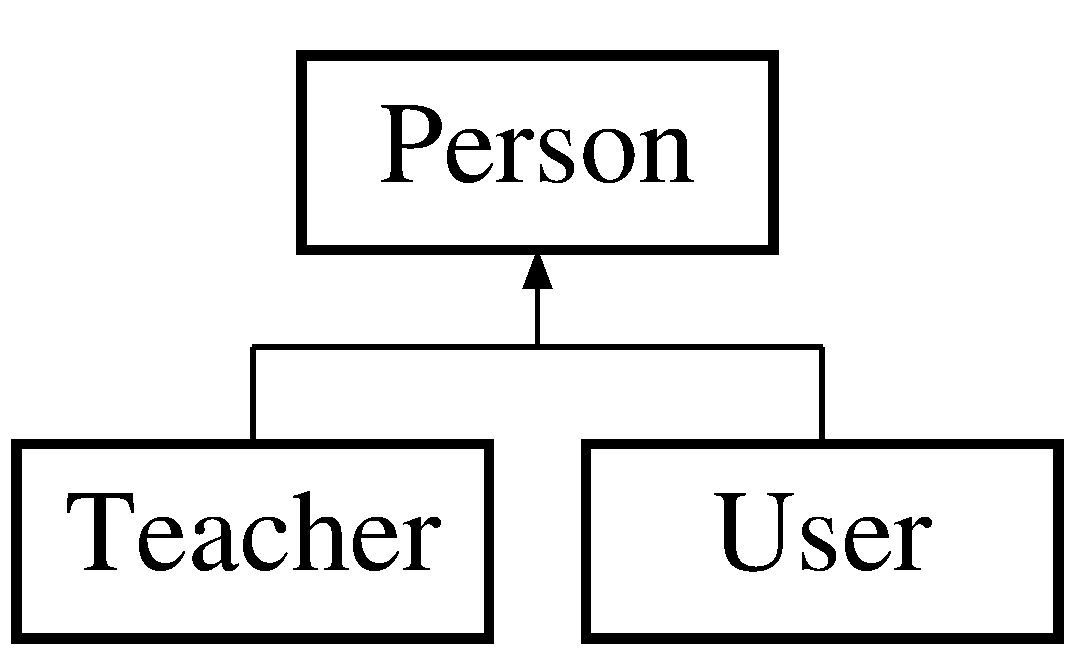
\includegraphics[height=2.000000cm]{class_person}
\end{center}
\end{figure}
\subsection*{Public Member Functions}
\begin{DoxyCompactItemize}
\item 
\mbox{\Hypertarget{class_person_a0397c6f89fafc12e738923f612bc41a3}\label{class_person_a0397c6f89fafc12e738923f612bc41a3}} 
\mbox{\hyperlink{class_person_a0397c6f89fafc12e738923f612bc41a3}{Person}} ()
\begin{DoxyCompactList}\small\item\em Constructor of the class. \end{DoxyCompactList}\item 
\mbox{\hyperlink{class_person_a19ba5bb7e92c776268b3d453b4ef55b2}{Person}} (std\+::string name, int age, std\+::string gender)
\begin{DoxyCompactList}\small\item\em Constructor of the class. \end{DoxyCompactList}\item 
std\+::string \mbox{\hyperlink{class_person_a9db2e2ccfc6cfa0d7979613ec2aaa922}{get\+Name}} () const
\begin{DoxyCompactList}\small\item\em Getter of the name of the person. \end{DoxyCompactList}\item 
int \mbox{\hyperlink{class_person_a69b1611320c68967067747c91783d883}{get\+Age}} ()
\begin{DoxyCompactList}\small\item\em Getter of the age of the person. \end{DoxyCompactList}\item 
std\+::string \mbox{\hyperlink{class_person_a66e13299dd684b80e7f8a9303c751ad5}{get\+Gender}} ()
\begin{DoxyCompactList}\small\item\em Getter of the gender of the person. \end{DoxyCompactList}\item 
void \mbox{\hyperlink{class_person_ad6e438f456d3ae6f5b477931c0a6aeba}{set\+Name}} (std\+::string name)
\begin{DoxyCompactList}\small\item\em Setter of the name of the person. \end{DoxyCompactList}\item 
void \mbox{\hyperlink{class_person_ac8ade54c27a0657c987c395ff04a9d46}{set\+Age}} (int age)
\begin{DoxyCompactList}\small\item\em Setter of the age of the person. \end{DoxyCompactList}\item 
void \mbox{\hyperlink{class_person_a7625b600d2c9c0b9c9fc060a6906dac6}{set\+Gender}} (std\+::string gender)
\begin{DoxyCompactList}\small\item\em Setter of the gender of the person. \end{DoxyCompactList}\item 
virtual void \mbox{\hyperlink{class_person_a80f87df3f644706c2ad8fc8b800fdd95}{store\+Info}} (std\+::ofstream \&outfile, int \&indentation)
\begin{DoxyCompactList}\small\item\em Store in the information of the \mbox{\hyperlink{class_person}{Person}} to a file. \end{DoxyCompactList}\item 
virtual void \mbox{\hyperlink{class_person_af07a032df8d56dddade4dc43960b536b}{load\+Class}} (std\+::ifstream \&inpfile)
\begin{DoxyCompactList}\small\item\em Reading the information of a \mbox{\hyperlink{class_user}{User}} from a file. \end{DoxyCompactList}\item 
\mbox{\Hypertarget{class_person_a2f1231629a6e7e8c83ada57628e80a89}\label{class_person_a2f1231629a6e7e8c83ada57628e80a89}} 
virtual void \mbox{\hyperlink{class_person_a2f1231629a6e7e8c83ada57628e80a89}{show}} ()
\begin{DoxyCompactList}\small\item\em Showing the information of the person on the screen. \end{DoxyCompactList}\item 
bool \mbox{\hyperlink{class_person_aa2fe338cbcf08ee5981dce811fd3a50a}{operator==}} (const \mbox{\hyperlink{class_person}{Person}} \&p1)
\begin{DoxyCompactList}\small\item\em Comparing two People. \end{DoxyCompactList}\end{DoxyCompactItemize}


\subsection{Detailed Description}
The class that stores the information of the people in the company 

\subsection{Constructor \& Destructor Documentation}
\mbox{\Hypertarget{class_person_a19ba5bb7e92c776268b3d453b4ef55b2}\label{class_person_a19ba5bb7e92c776268b3d453b4ef55b2}} 
\index{Person@{Person}!Person@{Person}}
\index{Person@{Person}!Person@{Person}}
\subsubsection{\texorpdfstring{Person()}{Person()}}
{\footnotesize\ttfamily Person\+::\+Person (\begin{DoxyParamCaption}\item[{std\+::string}]{name,  }\item[{int}]{age,  }\item[{std\+::string}]{gender }\end{DoxyParamCaption})}



Constructor of the class. 


\begin{DoxyParams}{Parameters}
{\em name} & -\/ name of the person \\
\hline
{\em age} & -\/ age of the person \\
\hline
{\em gender} & -\/ gender of the person \\
\hline
\end{DoxyParams}


\subsection{Member Function Documentation}
\mbox{\Hypertarget{class_person_a69b1611320c68967067747c91783d883}\label{class_person_a69b1611320c68967067747c91783d883}} 
\index{Person@{Person}!get\+Age@{get\+Age}}
\index{get\+Age@{get\+Age}!Person@{Person}}
\subsubsection{\texorpdfstring{get\+Age()}{getAge()}}
{\footnotesize\ttfamily int Person\+::get\+Age (\begin{DoxyParamCaption}{ }\end{DoxyParamCaption})}



Getter of the age of the person. 

\begin{DoxyReturn}{Returns}
age of the person 
\end{DoxyReturn}
\mbox{\Hypertarget{class_person_a66e13299dd684b80e7f8a9303c751ad5}\label{class_person_a66e13299dd684b80e7f8a9303c751ad5}} 
\index{Person@{Person}!get\+Gender@{get\+Gender}}
\index{get\+Gender@{get\+Gender}!Person@{Person}}
\subsubsection{\texorpdfstring{get\+Gender()}{getGender()}}
{\footnotesize\ttfamily string Person\+::get\+Gender (\begin{DoxyParamCaption}{ }\end{DoxyParamCaption})}



Getter of the gender of the person. 

\begin{DoxyReturn}{Returns}
gender of the person 
\end{DoxyReturn}
\mbox{\Hypertarget{class_person_a9db2e2ccfc6cfa0d7979613ec2aaa922}\label{class_person_a9db2e2ccfc6cfa0d7979613ec2aaa922}} 
\index{Person@{Person}!get\+Name@{get\+Name}}
\index{get\+Name@{get\+Name}!Person@{Person}}
\subsubsection{\texorpdfstring{get\+Name()}{getName()}}
{\footnotesize\ttfamily string Person\+::get\+Name (\begin{DoxyParamCaption}{ }\end{DoxyParamCaption}) const}



Getter of the name of the person. 

\begin{DoxyReturn}{Returns}
name of the person 
\end{DoxyReturn}
\mbox{\Hypertarget{class_person_af07a032df8d56dddade4dc43960b536b}\label{class_person_af07a032df8d56dddade4dc43960b536b}} 
\index{Person@{Person}!load\+Class@{load\+Class}}
\index{load\+Class@{load\+Class}!Person@{Person}}
\subsubsection{\texorpdfstring{load\+Class()}{loadClass()}}
{\footnotesize\ttfamily void Person\+::load\+Class (\begin{DoxyParamCaption}\item[{std\+::ifstream \&}]{inpfile }\end{DoxyParamCaption})\hspace{0.3cm}{\ttfamily [virtual]}}



Reading the information of a \mbox{\hyperlink{class_user}{User}} from a file. 


\begin{DoxyParams}{Parameters}
{\em infile} & -\/ file to read the information from \\
\hline
\end{DoxyParams}


Reimplemented in \mbox{\hyperlink{class_teacher_a1f204644af41c43ff3bd0582393062fa}{Teacher}}, and \mbox{\hyperlink{class_user_abc12a9ca668bd860a3d6d2ae4791997d}{User}}.

\mbox{\Hypertarget{class_person_aa2fe338cbcf08ee5981dce811fd3a50a}\label{class_person_aa2fe338cbcf08ee5981dce811fd3a50a}} 
\index{Person@{Person}!operator==@{operator==}}
\index{operator==@{operator==}!Person@{Person}}
\subsubsection{\texorpdfstring{operator==()}{operator==()}}
{\footnotesize\ttfamily bool Person\+::operator== (\begin{DoxyParamCaption}\item[{const \mbox{\hyperlink{class_person}{Person}} \&}]{p1 }\end{DoxyParamCaption})}



Comparing two People. 


\begin{DoxyParams}{Parameters}
{\em p1} & -\/ the other person \\
\hline
\end{DoxyParams}
\begin{DoxyReturn}{Returns}

\end{DoxyReturn}
\mbox{\Hypertarget{class_person_ac8ade54c27a0657c987c395ff04a9d46}\label{class_person_ac8ade54c27a0657c987c395ff04a9d46}} 
\index{Person@{Person}!set\+Age@{set\+Age}}
\index{set\+Age@{set\+Age}!Person@{Person}}
\subsubsection{\texorpdfstring{set\+Age()}{setAge()}}
{\footnotesize\ttfamily void Person\+::set\+Age (\begin{DoxyParamCaption}\item[{int}]{age }\end{DoxyParamCaption})}



Setter of the age of the person. 


\begin{DoxyParams}{Parameters}
{\em age} & -\/ age of the person \\
\hline
\end{DoxyParams}
\mbox{\Hypertarget{class_person_a7625b600d2c9c0b9c9fc060a6906dac6}\label{class_person_a7625b600d2c9c0b9c9fc060a6906dac6}} 
\index{Person@{Person}!set\+Gender@{set\+Gender}}
\index{set\+Gender@{set\+Gender}!Person@{Person}}
\subsubsection{\texorpdfstring{set\+Gender()}{setGender()}}
{\footnotesize\ttfamily void Person\+::set\+Gender (\begin{DoxyParamCaption}\item[{std\+::string}]{gender }\end{DoxyParamCaption})}



Setter of the gender of the person. 


\begin{DoxyParams}{Parameters}
{\em gender} & -\/ gender of the person \\
\hline
\end{DoxyParams}
\mbox{\Hypertarget{class_person_ad6e438f456d3ae6f5b477931c0a6aeba}\label{class_person_ad6e438f456d3ae6f5b477931c0a6aeba}} 
\index{Person@{Person}!set\+Name@{set\+Name}}
\index{set\+Name@{set\+Name}!Person@{Person}}
\subsubsection{\texorpdfstring{set\+Name()}{setName()}}
{\footnotesize\ttfamily void Person\+::set\+Name (\begin{DoxyParamCaption}\item[{std\+::string}]{name }\end{DoxyParamCaption})}



Setter of the name of the person. 


\begin{DoxyParams}{Parameters}
{\em name} & -\/ name of the person \\
\hline
\end{DoxyParams}
\mbox{\Hypertarget{class_person_a80f87df3f644706c2ad8fc8b800fdd95}\label{class_person_a80f87df3f644706c2ad8fc8b800fdd95}} 
\index{Person@{Person}!store\+Info@{store\+Info}}
\index{store\+Info@{store\+Info}!Person@{Person}}
\subsubsection{\texorpdfstring{store\+Info()}{storeInfo()}}
{\footnotesize\ttfamily void Person\+::store\+Info (\begin{DoxyParamCaption}\item[{std\+::ofstream \&}]{outfile,  }\item[{int \&}]{indentation }\end{DoxyParamCaption})\hspace{0.3cm}{\ttfamily [virtual]}}



Store in the information of the \mbox{\hyperlink{class_person}{Person}} to a file. 


\begin{DoxyParams}{Parameters}
{\em outfile} & -\/ the file to write information \\
\hline
{\em indent} & -\/ current indentation \\
\hline
\end{DoxyParams}


Reimplemented in \mbox{\hyperlink{class_teacher_a2ece0d60fa7ec4aaf93333aa0be0d25f}{Teacher}}, and \mbox{\hyperlink{class_user_aac5ff0f6899f3ce56d1b2d12ed557c79}{User}}.



The documentation for this class was generated from the following files\+:\begin{DoxyCompactItemize}
\item 
Person.\+h\item 
Person.\+cpp\end{DoxyCompactItemize}

\hypertarget{class_report}{}\section{Report Class Reference}
\label{class_report}\index{Report@{Report}}


{\ttfamily \#include $<$Report.\+h$>$}

\subsection*{Public Member Functions}
\begin{DoxyCompactItemize}
\item 
\mbox{\Hypertarget{class_report_ae3150817fcf4ebf814358baf5bd72e8f}\label{class_report_ae3150817fcf4ebf814358baf5bd72e8f}} 
\mbox{\hyperlink{class_report_ae3150817fcf4ebf814358baf5bd72e8f}{Report}} ()
\begin{DoxyCompactList}\small\item\em Class Constructor. \end{DoxyCompactList}\item 
\mbox{\hyperlink{class_report_afb6a4377db483370b342b18211008664}{Report}} (std\+::string user\+Name, std\+::string teacher\+Name, const std\+::vector$<$ \mbox{\hyperlink{class_reservation}{Reservation}} $\ast$$>$ \&reservs)
\begin{DoxyCompactList}\small\item\em Class Constructor. \end{DoxyCompactList}\item 
std\+::string \mbox{\hyperlink{class_report_aaeac48b6c10c5bbf240fc518b6d45d05}{get\+Name}} ()
\begin{DoxyCompactList}\small\item\em Getter of the name of the \mbox{\hyperlink{class_user}{User}}. \end{DoxyCompactList}\item 
std\+::string \mbox{\hyperlink{class_report_af7c52b70f5fe6feae64e44affa6095cd}{get\+Teacher\+Name}} ()
\begin{DoxyCompactList}\small\item\em Getter of the name of the teacher. \end{DoxyCompactList}\item 
int \mbox{\hyperlink{class_report_a56fcac206c401ebc51d35fbe907ad729}{get\+Grade}} ()
\begin{DoxyCompactList}\small\item\em getter of the Grade \end{DoxyCompactList}\item 
std\+::vector$<$ \mbox{\hyperlink{class_reservation}{Reservation}} $\ast$ $>$ \mbox{\hyperlink{class_report_a2915547d50dfefb1eae33f12ed0942d8}{get\+Lessons}} ()
\begin{DoxyCompactList}\small\item\em Getter of the name of the Lessons. \end{DoxyCompactList}\item 
void \mbox{\hyperlink{class_report_a67a10004cf149f202015d55a14efe6c1}{indentation}} (std\+::ofstream \&outfile, int indent)
\begin{DoxyCompactList}\small\item\em Indenting the file. \end{DoxyCompactList}\item 
void \mbox{\hyperlink{class_report_ad36785f4f4531404a6464c6d5ce5a69b}{read\+Info}} (std\+::ifstream \&infile)
\begin{DoxyCompactList}\small\item\em Store in the information of the report to a file. \end{DoxyCompactList}\item 
void \mbox{\hyperlink{class_report_a47faf2023bd07e59ab0296e8d0b2d512}{store\+Info}} (std\+::ofstream \&outfile, int indent)
\begin{DoxyCompactList}\small\item\em Reading the information of a \mbox{\hyperlink{class_report}{Report}} from a file. \end{DoxyCompactList}\item 
std\+::string \mbox{\hyperlink{class_report_ac47731e5f3f0f22574223a2a9e5688b5}{get\+Hour\+Format}} (double hour)
\begin{DoxyCompactList}\small\item\em get the format of the Hour as wanted \end{DoxyCompactList}\end{DoxyCompactItemize}
\subsection*{Friends}
\begin{DoxyCompactItemize}
\item 
std\+::ostream \& \mbox{\hyperlink{class_report_a9c2eaa693abfadab4a6e151daee874e4}{operator$<$$<$}} (std\+::ostream \&os, \mbox{\hyperlink{class_report}{Report}} r)
\begin{DoxyCompactList}\small\item\em Writer of the information of the \mbox{\hyperlink{class_report}{Report}}. \end{DoxyCompactList}\end{DoxyCompactItemize}


\subsection{Detailed Description}
\mbox{\hyperlink{class_report}{Report}} of how the user did during this last month 

\subsection{Constructor \& Destructor Documentation}
\mbox{\Hypertarget{class_report_afb6a4377db483370b342b18211008664}\label{class_report_afb6a4377db483370b342b18211008664}} 
\index{Report@{Report}!Report@{Report}}
\index{Report@{Report}!Report@{Report}}
\subsubsection{\texorpdfstring{Report()}{Report()}}
{\footnotesize\ttfamily Report\+::\+Report (\begin{DoxyParamCaption}\item[{std\+::string}]{user\+Name,  }\item[{std\+::string}]{teacher\+Name,  }\item[{const std\+::vector$<$ \mbox{\hyperlink{class_reservation}{Reservation}} $\ast$$>$ \&}]{reservs }\end{DoxyParamCaption})}



Class Constructor. 


\begin{DoxyParams}{Parameters}
{\em user\+Name} & -\/ name of the user \\
\hline
{\em teacher\+Name} & -\/ name of the teacher \\
\hline
{\em reservs} & -\/ the reservations \\
\hline
\end{DoxyParams}


\subsection{Member Function Documentation}
\mbox{\Hypertarget{class_report_a56fcac206c401ebc51d35fbe907ad729}\label{class_report_a56fcac206c401ebc51d35fbe907ad729}} 
\index{Report@{Report}!get\+Grade@{get\+Grade}}
\index{get\+Grade@{get\+Grade}!Report@{Report}}
\subsubsection{\texorpdfstring{get\+Grade()}{getGrade()}}
{\footnotesize\ttfamily int Report\+::get\+Grade (\begin{DoxyParamCaption}{ }\end{DoxyParamCaption})}



getter of the Grade 

\begin{DoxyReturn}{Returns}
the grade itself 
\end{DoxyReturn}
\mbox{\Hypertarget{class_report_ac47731e5f3f0f22574223a2a9e5688b5}\label{class_report_ac47731e5f3f0f22574223a2a9e5688b5}} 
\index{Report@{Report}!get\+Hour\+Format@{get\+Hour\+Format}}
\index{get\+Hour\+Format@{get\+Hour\+Format}!Report@{Report}}
\subsubsection{\texorpdfstring{get\+Hour\+Format()}{getHourFormat()}}
{\footnotesize\ttfamily string Report\+::get\+Hour\+Format (\begin{DoxyParamCaption}\item[{double}]{hour }\end{DoxyParamCaption})}



get the format of the Hour as wanted 


\begin{DoxyParams}{Parameters}
{\em hour} & -\/ the actual time \\
\hline
\end{DoxyParams}
\begin{DoxyReturn}{Returns}
the hour 
\end{DoxyReturn}
\mbox{\Hypertarget{class_report_a2915547d50dfefb1eae33f12ed0942d8}\label{class_report_a2915547d50dfefb1eae33f12ed0942d8}} 
\index{Report@{Report}!get\+Lessons@{get\+Lessons}}
\index{get\+Lessons@{get\+Lessons}!Report@{Report}}
\subsubsection{\texorpdfstring{get\+Lessons()}{getLessons()}}
{\footnotesize\ttfamily vector$<$ \mbox{\hyperlink{class_reservation}{Reservation}} $\ast$ $>$ Report\+::get\+Lessons (\begin{DoxyParamCaption}{ }\end{DoxyParamCaption})}



Getter of the name of the Lessons. 

\begin{DoxyReturn}{Returns}
the vector of reservations 
\end{DoxyReturn}
\mbox{\Hypertarget{class_report_aaeac48b6c10c5bbf240fc518b6d45d05}\label{class_report_aaeac48b6c10c5bbf240fc518b6d45d05}} 
\index{Report@{Report}!get\+Name@{get\+Name}}
\index{get\+Name@{get\+Name}!Report@{Report}}
\subsubsection{\texorpdfstring{get\+Name()}{getName()}}
{\footnotesize\ttfamily string Report\+::get\+Name (\begin{DoxyParamCaption}{ }\end{DoxyParamCaption})}



Getter of the name of the \mbox{\hyperlink{class_user}{User}}. 

\begin{DoxyReturn}{Returns}
the name of the \mbox{\hyperlink{class_user}{User}} 
\end{DoxyReturn}
\mbox{\Hypertarget{class_report_af7c52b70f5fe6feae64e44affa6095cd}\label{class_report_af7c52b70f5fe6feae64e44affa6095cd}} 
\index{Report@{Report}!get\+Teacher\+Name@{get\+Teacher\+Name}}
\index{get\+Teacher\+Name@{get\+Teacher\+Name}!Report@{Report}}
\subsubsection{\texorpdfstring{get\+Teacher\+Name()}{getTeacherName()}}
{\footnotesize\ttfamily string Report\+::get\+Teacher\+Name (\begin{DoxyParamCaption}{ }\end{DoxyParamCaption})}



Getter of the name of the teacher. 

\begin{DoxyReturn}{Returns}
the name of the teacher 
\end{DoxyReturn}
\mbox{\Hypertarget{class_report_a67a10004cf149f202015d55a14efe6c1}\label{class_report_a67a10004cf149f202015d55a14efe6c1}} 
\index{Report@{Report}!indentation@{indentation}}
\index{indentation@{indentation}!Report@{Report}}
\subsubsection{\texorpdfstring{indentation()}{indentation()}}
{\footnotesize\ttfamily void Report\+::indentation (\begin{DoxyParamCaption}\item[{std\+::ofstream \&}]{outfile,  }\item[{int}]{indent }\end{DoxyParamCaption})}



Indenting the file. 


\begin{DoxyParams}{Parameters}
{\em outfile} & -\/ the file to write information \\
\hline
{\em indent} & -\/ current indentation \\
\hline
\end{DoxyParams}
\mbox{\Hypertarget{class_report_ad36785f4f4531404a6464c6d5ce5a69b}\label{class_report_ad36785f4f4531404a6464c6d5ce5a69b}} 
\index{Report@{Report}!read\+Info@{read\+Info}}
\index{read\+Info@{read\+Info}!Report@{Report}}
\subsubsection{\texorpdfstring{read\+Info()}{readInfo()}}
{\footnotesize\ttfamily void Report\+::read\+Info (\begin{DoxyParamCaption}\item[{std\+::ifstream \&}]{infile }\end{DoxyParamCaption})}



Store in the information of the report to a file. 


\begin{DoxyParams}{Parameters}
{\em outfile} & -\/ the file to write information \\
\hline
{\em indent} & -\/ current indentation \\
\hline
\end{DoxyParams}
\mbox{\Hypertarget{class_report_a47faf2023bd07e59ab0296e8d0b2d512}\label{class_report_a47faf2023bd07e59ab0296e8d0b2d512}} 
\index{Report@{Report}!store\+Info@{store\+Info}}
\index{store\+Info@{store\+Info}!Report@{Report}}
\subsubsection{\texorpdfstring{store\+Info()}{storeInfo()}}
{\footnotesize\ttfamily void Report\+::store\+Info (\begin{DoxyParamCaption}\item[{std\+::ofstream \&}]{outfile,  }\item[{int}]{indent }\end{DoxyParamCaption})}



Reading the information of a \mbox{\hyperlink{class_report}{Report}} from a file. 


\begin{DoxyParams}{Parameters}
{\em infile} & -\/ file to read the information from \\
\hline
\end{DoxyParams}


\subsection{Friends And Related Function Documentation}
\mbox{\Hypertarget{class_report_a9c2eaa693abfadab4a6e151daee874e4}\label{class_report_a9c2eaa693abfadab4a6e151daee874e4}} 
\index{Report@{Report}!operator$<$$<$@{operator$<$$<$}}
\index{operator$<$$<$@{operator$<$$<$}!Report@{Report}}
\subsubsection{\texorpdfstring{operator$<$$<$}{operator<<}}
{\footnotesize\ttfamily std\+::ostream\& operator$<$$<$ (\begin{DoxyParamCaption}\item[{std\+::ostream \&}]{os,  }\item[{\mbox{\hyperlink{class_report}{Report}}}]{r }\end{DoxyParamCaption})\hspace{0.3cm}{\ttfamily [friend]}}



Writer of the information of the \mbox{\hyperlink{class_report}{Report}}. 


\begin{DoxyParams}{Parameters}
{\em os} & -\/ the stream \\
\hline
{\em r} & -\/ the report itself \\
\hline
\end{DoxyParams}
\begin{DoxyReturn}{Returns}
the stream 
\end{DoxyReturn}


The documentation for this class was generated from the following files\+:\begin{DoxyCompactItemize}
\item 
Report.\+h\item 
Report.\+cpp\end{DoxyCompactItemize}

\hypertarget{class_report_already_exists}{}\section{Report\+Already\+Exists Class Reference}
\label{class_report_already_exists}\index{Report\+Already\+Exists@{Report\+Already\+Exists}}
\subsection*{Public Member Functions}
\begin{DoxyCompactItemize}
\item 
\mbox{\Hypertarget{class_report_already_exists_add9175e1939193586e63a421bf9d2870}\label{class_report_already_exists_add9175e1939193586e63a421bf9d2870}} 
{\bfseries Report\+Already\+Exists} (int month)
\item 
\mbox{\Hypertarget{class_report_already_exists_a1521d7f897144a910951b37f132cd922}\label{class_report_already_exists_a1521d7f897144a910951b37f132cd922}} 
int {\bfseries get\+Month} ()
\item 
\mbox{\Hypertarget{class_report_already_exists_a66103e5ca6a4b84f3492493b7ced740d}\label{class_report_already_exists_a66103e5ca6a4b84f3492493b7ced740d}} 
std\+::string {\bfseries what} () const
\end{DoxyCompactItemize}


The documentation for this class was generated from the following files\+:\begin{DoxyCompactItemize}
\item 
Person.\+h\item 
Person.\+cpp\end{DoxyCompactItemize}

\hypertarget{class_report_not_available}{}\section{Report\+Not\+Available Class Reference}
\label{class_report_not_available}\index{Report\+Not\+Available@{Report\+Not\+Available}}


{\ttfamily \#include $<$Person.\+h$>$}

\subsection*{Public Member Functions}
\begin{DoxyCompactItemize}
\item 
\mbox{\hyperlink{class_report_not_available_af8c20e04e062f7922f5507ca31d37854}{Report\+Not\+Available}} (int \mbox{\hyperlink{class_report_not_available_a11686bc53e58de31838b14e6a23ec0c6}{month}})
\item 
int \mbox{\hyperlink{class_report_not_available_a64bf230892d4e34fecb8143d04b95d02}{get\+Month}} ()
\item 
std\+::string \mbox{\hyperlink{class_report_not_available_a2139ebc44990ab772c6e56d0a0d71e7d}{what}} () const
\end{DoxyCompactItemize}
\subsection*{Public Attributes}
\begin{DoxyCompactItemize}
\item 
int \mbox{\hyperlink{class_report_not_available_a11686bc53e58de31838b14e6a23ec0c6}{month}}
\end{DoxyCompactItemize}


\subsection{Constructor \& Destructor Documentation}
\mbox{\Hypertarget{class_report_not_available_af8c20e04e062f7922f5507ca31d37854}\label{class_report_not_available_af8c20e04e062f7922f5507ca31d37854}} 
\index{Report\+Not\+Available@{Report\+Not\+Available}!Report\+Not\+Available@{Report\+Not\+Available}}
\index{Report\+Not\+Available@{Report\+Not\+Available}!Report\+Not\+Available@{Report\+Not\+Available}}
\subsubsection{\texorpdfstring{Report\+Not\+Available()}{ReportNotAvailable()}}
{\footnotesize\ttfamily Report\+Not\+Available\+::\+Report\+Not\+Available (\begin{DoxyParamCaption}\item[{int}]{month }\end{DoxyParamCaption})\hspace{0.3cm}{\ttfamily [inline]}}



\subsection{Member Function Documentation}
\mbox{\Hypertarget{class_report_not_available_a64bf230892d4e34fecb8143d04b95d02}\label{class_report_not_available_a64bf230892d4e34fecb8143d04b95d02}} 
\index{Report\+Not\+Available@{Report\+Not\+Available}!get\+Month@{get\+Month}}
\index{get\+Month@{get\+Month}!Report\+Not\+Available@{Report\+Not\+Available}}
\subsubsection{\texorpdfstring{get\+Month()}{getMonth()}}
{\footnotesize\ttfamily int Report\+Not\+Available\+::get\+Month (\begin{DoxyParamCaption}{ }\end{DoxyParamCaption})\hspace{0.3cm}{\ttfamily [inline]}}

\mbox{\Hypertarget{class_report_not_available_a2139ebc44990ab772c6e56d0a0d71e7d}\label{class_report_not_available_a2139ebc44990ab772c6e56d0a0d71e7d}} 
\index{Report\+Not\+Available@{Report\+Not\+Available}!what@{what}}
\index{what@{what}!Report\+Not\+Available@{Report\+Not\+Available}}
\subsubsection{\texorpdfstring{what()}{what()}}
{\footnotesize\ttfamily string Report\+Not\+Available\+::what (\begin{DoxyParamCaption}{ }\end{DoxyParamCaption}) const}



\subsection{Member Data Documentation}
\mbox{\Hypertarget{class_report_not_available_a11686bc53e58de31838b14e6a23ec0c6}\label{class_report_not_available_a11686bc53e58de31838b14e6a23ec0c6}} 
\index{Report\+Not\+Available@{Report\+Not\+Available}!month@{month}}
\index{month@{month}!Report\+Not\+Available@{Report\+Not\+Available}}
\subsubsection{\texorpdfstring{month}{month}}
{\footnotesize\ttfamily int Report\+Not\+Available\+::month}



The documentation for this class was generated from the following files\+:\begin{DoxyCompactItemize}
\item 
\mbox{\hyperlink{_person_8h}{Person.\+h}}\item 
\mbox{\hyperlink{_person_8cpp}{Person.\+cpp}}\end{DoxyCompactItemize}

\hypertarget{class_reservation}{}\section{Reservation Class Reference}
\label{class_reservation}\index{Reservation@{Reservation}}


{\ttfamily \#include $<$Reservation.\+h$>$}

Inheritance diagram for Reservation\+:\begin{figure}[H]
\begin{center}
\leavevmode
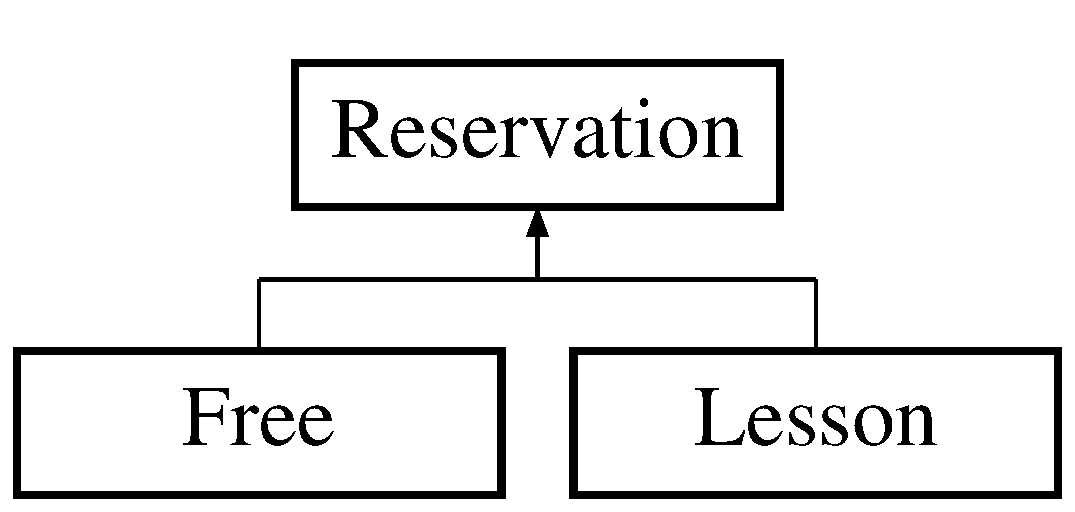
\includegraphics[height=2.000000cm]{class_reservation}
\end{center}
\end{figure}
\subsection*{Public Member Functions}
\begin{DoxyCompactItemize}
\item 
\mbox{\hyperlink{class_reservation_a63b283053695e6f50fa44c50da2b3de5}{Reservation}} ()
\begin{DoxyCompactList}\small\item\em Constructor of Class. \end{DoxyCompactList}\item 
\mbox{\hyperlink{class_reservation_ac060bb57009704f7cfe33bed498b72d0}{Reservation}} (int month, int day, int starting\+Hour, double \mbox{\hyperlink{class_reservation_a82e197bd30e7949ee9b8616ee4eacf83}{price}}, unsigned int \mbox{\hyperlink{class_reservation_a1a311bb23edebfa226f9c744aefdc7b1}{duration}})
\begin{DoxyCompactList}\small\item\em Constructor of Class. \end{DoxyCompactList}\item 
virtual double \mbox{\hyperlink{class_reservation_a62cdb2f1a24e2fce92fb9f024ae9f494}{get\+Price}} ()
\begin{DoxyCompactList}\small\item\em Method to obtain the price of the reservation. \end{DoxyCompactList}\item 
double \mbox{\hyperlink{class_reservation_a28da7b16dadfeb33bf5351cabc8dbb0b}{get\+Starting\+Hour}} ()
\begin{DoxyCompactList}\small\item\em Method to obtain the Starting Hour of the reservation. \end{DoxyCompactList}\item 
int \mbox{\hyperlink{class_reservation_a9d91ef1230af46952cb5422ae769bfa1}{get\+Duration}} ()
\begin{DoxyCompactList}\small\item\em Method to obtain the duration of the reservation. \end{DoxyCompactList}\item 
int \mbox{\hyperlink{class_reservation_adbc454654e7e861d80c8740f85e0fb10}{get\+Month}} ()
\begin{DoxyCompactList}\small\item\em Method to obtain the month of the reservation. \end{DoxyCompactList}\item 
int \mbox{\hyperlink{class_reservation_a22d66f6cc7532b775d5a05338ad6b196}{get\+Day}} ()
\begin{DoxyCompactList}\small\item\em Method to obtain the day of the reservation. \end{DoxyCompactList}\item 
bool \mbox{\hyperlink{class_reservation_ae033fc48c694b375e0cc68215f7dcfdb}{operator==}} (\mbox{\hyperlink{class_reservation}{Reservation}} \&r) const
\begin{DoxyCompactList}\small\item\em Implementation of the equal operator. \end{DoxyCompactList}\item 
virtual void \mbox{\hyperlink{class_reservation_a8ec83fe2eb15294c3a51a9998ed17df7}{store\+Info}} (std\+::ofstream \&outfile, int \mbox{\hyperlink{class_reservation_a480981ed050bae19bc74bbb0bbb459f9}{indent}})
\begin{DoxyCompactList}\small\item\em Store in the information of the reservation to a file. \end{DoxyCompactList}\item 
void \mbox{\hyperlink{class_reservation_a480981ed050bae19bc74bbb0bbb459f9}{indent}} (std\+::ofstream \&outfile, int indent)
\begin{DoxyCompactList}\small\item\em Indenting the file. \end{DoxyCompactList}\item 
virtual void \mbox{\hyperlink{class_reservation_acff32024a350c2156af9f74522c59b7b}{read\+Info}} (std\+::ifstream \&infile)
\begin{DoxyCompactList}\small\item\em Reading the information of a \mbox{\hyperlink{class_reservation}{Reservation}} from a file. \end{DoxyCompactList}\end{DoxyCompactItemize}
\subsection*{Protected Attributes}
\begin{DoxyCompactItemize}
\item 
double \mbox{\hyperlink{class_reservation_a82e197bd30e7949ee9b8616ee4eacf83}{price}}
\item 
unsigned int \mbox{\hyperlink{class_reservation_a1a311bb23edebfa226f9c744aefdc7b1}{duration}}
\end{DoxyCompactItemize}


\subsection{Detailed Description}
The reservation of a court, to be stored on the people that will be on that court 

\subsection{Constructor \& Destructor Documentation}
\mbox{\Hypertarget{class_reservation_a63b283053695e6f50fa44c50da2b3de5}\label{class_reservation_a63b283053695e6f50fa44c50da2b3de5}} 
\index{Reservation@{Reservation}!Reservation@{Reservation}}
\index{Reservation@{Reservation}!Reservation@{Reservation}}
\subsubsection{\texorpdfstring{Reservation()}{Reservation()}\hspace{0.1cm}{\footnotesize\ttfamily [1/2]}}
{\footnotesize\ttfamily Reservation\+::\+Reservation (\begin{DoxyParamCaption}{ }\end{DoxyParamCaption})\hspace{0.3cm}{\ttfamily [inline]}}



Constructor of Class. 

\mbox{\Hypertarget{class_reservation_ac060bb57009704f7cfe33bed498b72d0}\label{class_reservation_ac060bb57009704f7cfe33bed498b72d0}} 
\index{Reservation@{Reservation}!Reservation@{Reservation}}
\index{Reservation@{Reservation}!Reservation@{Reservation}}
\subsubsection{\texorpdfstring{Reservation()}{Reservation()}\hspace{0.1cm}{\footnotesize\ttfamily [2/2]}}
{\footnotesize\ttfamily Reservation\+::\+Reservation (\begin{DoxyParamCaption}\item[{int}]{month,  }\item[{int}]{day,  }\item[{int}]{starting\+Hour,  }\item[{double}]{price,  }\item[{unsigned int}]{duration }\end{DoxyParamCaption})}



Constructor of Class. 


\begin{DoxyParams}{Parameters}
{\em month} & -\/ \mbox{\hyperlink{class_month}{Month}} of the reservation \\
\hline
{\em day} & -\/ \mbox{\hyperlink{class_day}{Day}} of the reservation \\
\hline
{\em starting\+Hour} & -\/ Starting Hour of the reservation \\
\hline
{\em price} & -\/ Price of the reservation \\
\hline
{\em duration} & -\/ Duration of the reservation \\
\hline
\end{DoxyParams}


\subsection{Member Function Documentation}
\mbox{\Hypertarget{class_reservation_a22d66f6cc7532b775d5a05338ad6b196}\label{class_reservation_a22d66f6cc7532b775d5a05338ad6b196}} 
\index{Reservation@{Reservation}!get\+Day@{get\+Day}}
\index{get\+Day@{get\+Day}!Reservation@{Reservation}}
\subsubsection{\texorpdfstring{get\+Day()}{getDay()}}
{\footnotesize\ttfamily int Reservation\+::get\+Day (\begin{DoxyParamCaption}{ }\end{DoxyParamCaption})}



Method to obtain the day of the reservation. 

\begin{DoxyReturn}{Returns}
\mbox{\hyperlink{class_day}{Day}} of the reservation 
\end{DoxyReturn}
\mbox{\Hypertarget{class_reservation_a9d91ef1230af46952cb5422ae769bfa1}\label{class_reservation_a9d91ef1230af46952cb5422ae769bfa1}} 
\index{Reservation@{Reservation}!get\+Duration@{get\+Duration}}
\index{get\+Duration@{get\+Duration}!Reservation@{Reservation}}
\subsubsection{\texorpdfstring{get\+Duration()}{getDuration()}}
{\footnotesize\ttfamily int Reservation\+::get\+Duration (\begin{DoxyParamCaption}{ }\end{DoxyParamCaption})}



Method to obtain the duration of the reservation. 

\begin{DoxyReturn}{Returns}
Duration of the reservation 
\end{DoxyReturn}
\mbox{\Hypertarget{class_reservation_adbc454654e7e861d80c8740f85e0fb10}\label{class_reservation_adbc454654e7e861d80c8740f85e0fb10}} 
\index{Reservation@{Reservation}!get\+Month@{get\+Month}}
\index{get\+Month@{get\+Month}!Reservation@{Reservation}}
\subsubsection{\texorpdfstring{get\+Month()}{getMonth()}}
{\footnotesize\ttfamily int Reservation\+::get\+Month (\begin{DoxyParamCaption}{ }\end{DoxyParamCaption})}



Method to obtain the month of the reservation. 

\begin{DoxyReturn}{Returns}
\mbox{\hyperlink{class_month}{Month}} of the reservation 
\end{DoxyReturn}
\mbox{\Hypertarget{class_reservation_a62cdb2f1a24e2fce92fb9f024ae9f494}\label{class_reservation_a62cdb2f1a24e2fce92fb9f024ae9f494}} 
\index{Reservation@{Reservation}!get\+Price@{get\+Price}}
\index{get\+Price@{get\+Price}!Reservation@{Reservation}}
\subsubsection{\texorpdfstring{get\+Price()}{getPrice()}}
{\footnotesize\ttfamily double Reservation\+::get\+Price (\begin{DoxyParamCaption}{ }\end{DoxyParamCaption})\hspace{0.3cm}{\ttfamily [virtual]}}



Method to obtain the price of the reservation. 

\begin{DoxyReturn}{Returns}
Price of the reservation 
\end{DoxyReturn}


Reimplemented in \mbox{\hyperlink{class_free_a229f009a7535eeba0a6ff4495de8c6bf}{Free}}, and \mbox{\hyperlink{class_lesson_ad7a2f708f870040627a442cdf000683f}{Lesson}}.

\mbox{\Hypertarget{class_reservation_a28da7b16dadfeb33bf5351cabc8dbb0b}\label{class_reservation_a28da7b16dadfeb33bf5351cabc8dbb0b}} 
\index{Reservation@{Reservation}!get\+Starting\+Hour@{get\+Starting\+Hour}}
\index{get\+Starting\+Hour@{get\+Starting\+Hour}!Reservation@{Reservation}}
\subsubsection{\texorpdfstring{get\+Starting\+Hour()}{getStartingHour()}}
{\footnotesize\ttfamily double Reservation\+::get\+Starting\+Hour (\begin{DoxyParamCaption}{ }\end{DoxyParamCaption})}



Method to obtain the Starting Hour of the reservation. 

\begin{DoxyReturn}{Returns}
Starting Hour of the reservation 
\end{DoxyReturn}
\mbox{\Hypertarget{class_reservation_a480981ed050bae19bc74bbb0bbb459f9}\label{class_reservation_a480981ed050bae19bc74bbb0bbb459f9}} 
\index{Reservation@{Reservation}!indent@{indent}}
\index{indent@{indent}!Reservation@{Reservation}}
\subsubsection{\texorpdfstring{indent()}{indent()}}
{\footnotesize\ttfamily void Reservation\+::indent (\begin{DoxyParamCaption}\item[{std\+::ofstream \&}]{outfile,  }\item[{int}]{indent }\end{DoxyParamCaption})}



Indenting the file. 


\begin{DoxyParams}{Parameters}
{\em outfile} & -\/ the file to write information \\
\hline
{\em indent} & -\/ current indentation \\
\hline
\end{DoxyParams}
\mbox{\Hypertarget{class_reservation_ae033fc48c694b375e0cc68215f7dcfdb}\label{class_reservation_ae033fc48c694b375e0cc68215f7dcfdb}} 
\index{Reservation@{Reservation}!operator==@{operator==}}
\index{operator==@{operator==}!Reservation@{Reservation}}
\subsubsection{\texorpdfstring{operator==()}{operator==()}}
{\footnotesize\ttfamily bool Reservation\+::operator== (\begin{DoxyParamCaption}\item[{\mbox{\hyperlink{class_reservation}{Reservation}} \&}]{r }\end{DoxyParamCaption}) const}



Implementation of the equal operator. 


\begin{DoxyParams}{Parameters}
{\em r} & -\/ the other reservation \\
\hline
\end{DoxyParams}
\begin{DoxyReturn}{Returns}
if -\/ the reservation is the same 
\end{DoxyReturn}
\mbox{\Hypertarget{class_reservation_acff32024a350c2156af9f74522c59b7b}\label{class_reservation_acff32024a350c2156af9f74522c59b7b}} 
\index{Reservation@{Reservation}!read\+Info@{read\+Info}}
\index{read\+Info@{read\+Info}!Reservation@{Reservation}}
\subsubsection{\texorpdfstring{read\+Info()}{readInfo()}}
{\footnotesize\ttfamily void Reservation\+::read\+Info (\begin{DoxyParamCaption}\item[{std\+::ifstream \&}]{infile }\end{DoxyParamCaption})\hspace{0.3cm}{\ttfamily [virtual]}}



Reading the information of a \mbox{\hyperlink{class_reservation}{Reservation}} from a file. 


\begin{DoxyParams}{Parameters}
{\em infile} & -\/ file to read the information from \\
\hline
\end{DoxyParams}


Reimplemented in \mbox{\hyperlink{class_free_ad1023c825c9790edf0797e2e69dd2fcf}{Free}}, and \mbox{\hyperlink{class_lesson_a3ac64e2f79bc9e381634d5d30499e8f1}{Lesson}}.

\mbox{\Hypertarget{class_reservation_a8ec83fe2eb15294c3a51a9998ed17df7}\label{class_reservation_a8ec83fe2eb15294c3a51a9998ed17df7}} 
\index{Reservation@{Reservation}!store\+Info@{store\+Info}}
\index{store\+Info@{store\+Info}!Reservation@{Reservation}}
\subsubsection{\texorpdfstring{store\+Info()}{storeInfo()}}
{\footnotesize\ttfamily void Reservation\+::store\+Info (\begin{DoxyParamCaption}\item[{std\+::ofstream \&}]{outfile,  }\item[{int}]{indent }\end{DoxyParamCaption})\hspace{0.3cm}{\ttfamily [virtual]}}



Store in the information of the reservation to a file. 


\begin{DoxyParams}{Parameters}
{\em outfile} & -\/ the file to write information \\
\hline
{\em indent} & -\/ current indentation \\
\hline
\end{DoxyParams}


Reimplemented in \mbox{\hyperlink{class_free_a5eec9da16ebf4f388d16dd270bd93b64}{Free}}, and \mbox{\hyperlink{class_lesson_a645855060ab3c915a6e0875bc5584887}{Lesson}}.



\subsection{Member Data Documentation}
\mbox{\Hypertarget{class_reservation_a1a311bb23edebfa226f9c744aefdc7b1}\label{class_reservation_a1a311bb23edebfa226f9c744aefdc7b1}} 
\index{Reservation@{Reservation}!duration@{duration}}
\index{duration@{duration}!Reservation@{Reservation}}
\subsubsection{\texorpdfstring{duration}{duration}}
{\footnotesize\ttfamily unsigned int Reservation\+::duration\hspace{0.3cm}{\ttfamily [protected]}}

Duration of said reservation \mbox{\Hypertarget{class_reservation_a82e197bd30e7949ee9b8616ee4eacf83}\label{class_reservation_a82e197bd30e7949ee9b8616ee4eacf83}} 
\index{Reservation@{Reservation}!price@{price}}
\index{price@{price}!Reservation@{Reservation}}
\subsubsection{\texorpdfstring{price}{price}}
{\footnotesize\ttfamily double Reservation\+::price\hspace{0.3cm}{\ttfamily [protected]}}

Price associated of the reservation 

The documentation for this class was generated from the following files\+:\begin{DoxyCompactItemize}
\item 
\mbox{\hyperlink{_reservation_8h}{Reservation.\+h}}\item 
\mbox{\hyperlink{_reservation_8cpp}{Reservation.\+cpp}}\end{DoxyCompactItemize}

\hypertarget{class_start_hour_inside_res}{}\section{Start\+Hour\+Inside\+Res Class Reference}
\label{class_start_hour_inside_res}\index{Start\+Hour\+Inside\+Res@{Start\+Hour\+Inside\+Res}}


{\ttfamily \#include $<$Person.\+h$>$}

Inheritance diagram for Start\+Hour\+Inside\+Res\+:\begin{figure}[H]
\begin{center}
\leavevmode
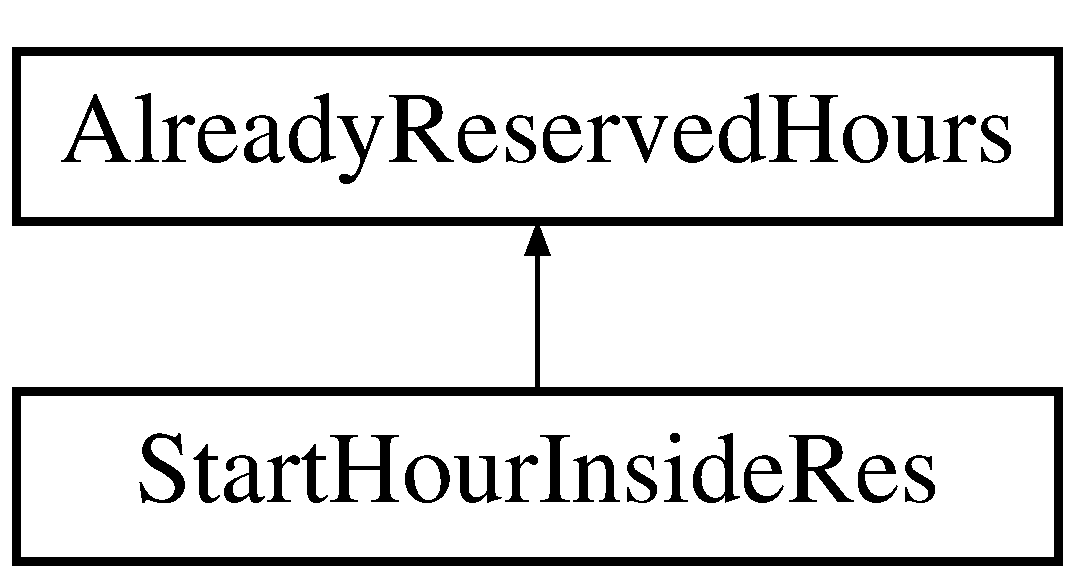
\includegraphics[height=2.000000cm]{class_start_hour_inside_res}
\end{center}
\end{figure}
\subsection*{Public Member Functions}
\begin{DoxyCompactItemize}
\item 
\mbox{\hyperlink{class_start_hour_inside_res_a6c05984e1473ec49ce644ecfaecab8fc}{Start\+Hour\+Inside\+Res}} (double Starting\+Hour, double end\+Hour)
\item 
std\+::string \mbox{\hyperlink{class_start_hour_inside_res_a90b45cf2a2d4f0adcf7d9f650bee1574}{what}} () const
\end{DoxyCompactItemize}


\subsection{Constructor \& Destructor Documentation}
\mbox{\Hypertarget{class_start_hour_inside_res_a6c05984e1473ec49ce644ecfaecab8fc}\label{class_start_hour_inside_res_a6c05984e1473ec49ce644ecfaecab8fc}} 
\index{Start\+Hour\+Inside\+Res@{Start\+Hour\+Inside\+Res}!Start\+Hour\+Inside\+Res@{Start\+Hour\+Inside\+Res}}
\index{Start\+Hour\+Inside\+Res@{Start\+Hour\+Inside\+Res}!Start\+Hour\+Inside\+Res@{Start\+Hour\+Inside\+Res}}
\subsubsection{\texorpdfstring{Start\+Hour\+Inside\+Res()}{StartHourInsideRes()}}
{\footnotesize\ttfamily Start\+Hour\+Inside\+Res\+::\+Start\+Hour\+Inside\+Res (\begin{DoxyParamCaption}\item[{double}]{Starting\+Hour,  }\item[{double}]{end\+Hour }\end{DoxyParamCaption})\hspace{0.3cm}{\ttfamily [inline]}}



\subsection{Member Function Documentation}
\mbox{\Hypertarget{class_start_hour_inside_res_a90b45cf2a2d4f0adcf7d9f650bee1574}\label{class_start_hour_inside_res_a90b45cf2a2d4f0adcf7d9f650bee1574}} 
\index{Start\+Hour\+Inside\+Res@{Start\+Hour\+Inside\+Res}!what@{what}}
\index{what@{what}!Start\+Hour\+Inside\+Res@{Start\+Hour\+Inside\+Res}}
\subsubsection{\texorpdfstring{what()}{what()}}
{\footnotesize\ttfamily string Start\+Hour\+Inside\+Res\+::what (\begin{DoxyParamCaption}{ }\end{DoxyParamCaption}) const\hspace{0.3cm}{\ttfamily [virtual]}}



Reimplemented from \mbox{\hyperlink{class_already_reserved_hours_a69081ef7e75aa68b9aa5c75d02fe2194}{Already\+Reserved\+Hours}}.



The documentation for this class was generated from the following files\+:\begin{DoxyCompactItemize}
\item 
\mbox{\hyperlink{_person_8h}{Person.\+h}}\item 
\mbox{\hyperlink{_person_8cpp}{Person.\+cpp}}\end{DoxyCompactItemize}

\hypertarget{class_teacher}{}\section{Teacher Class Reference}
\label{class_teacher}\index{Teacher@{Teacher}}


{\ttfamily \#include $<$Person.\+h$>$}

Inheritance diagram for Teacher\+:\begin{figure}[H]
\begin{center}
\leavevmode
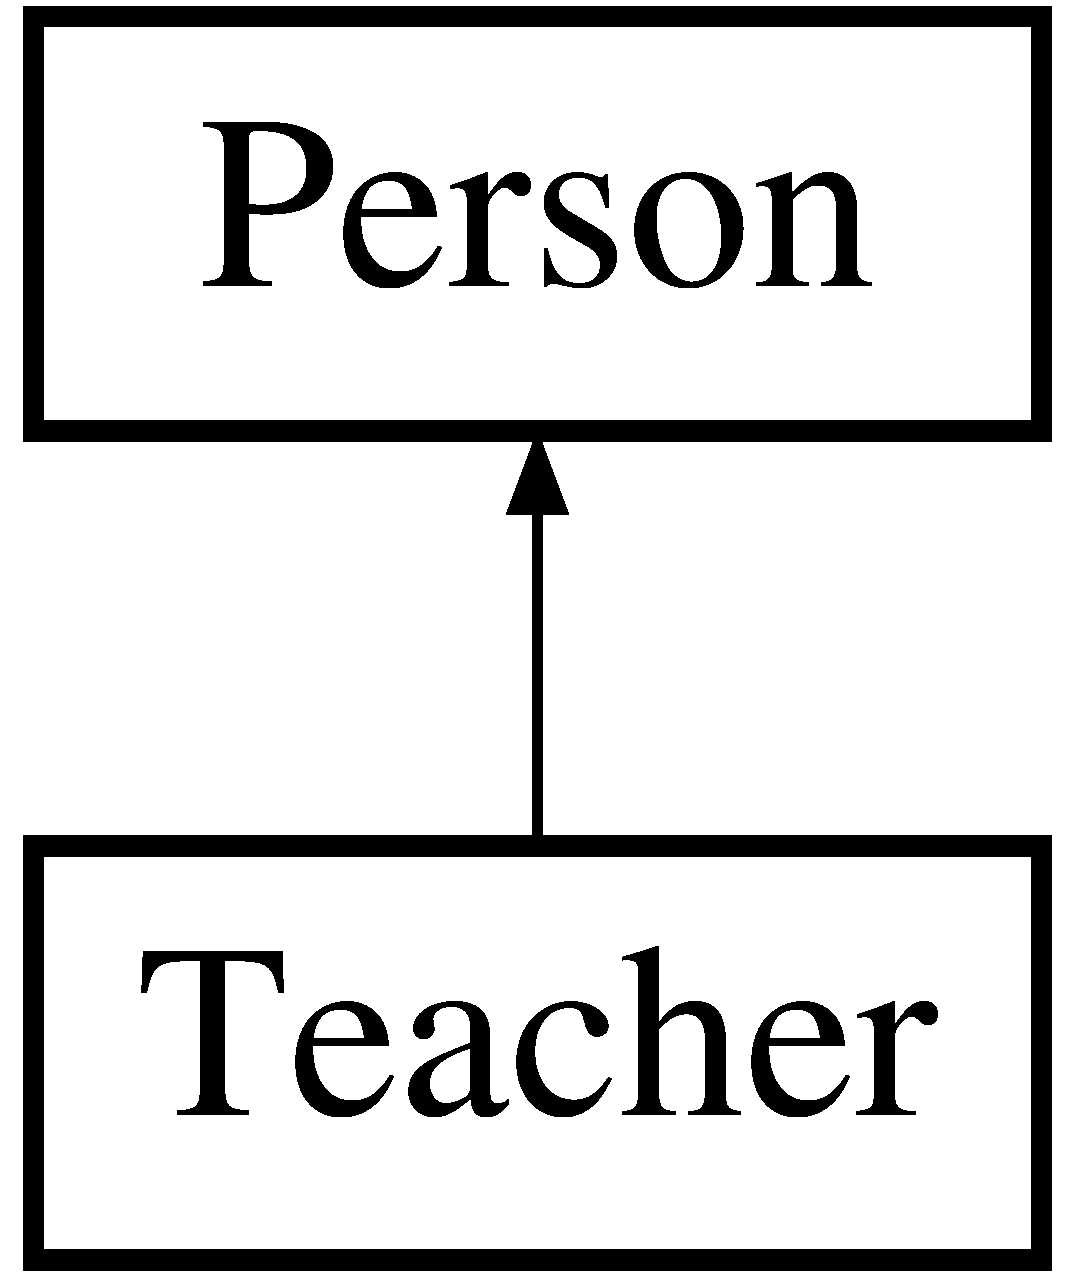
\includegraphics[height=2.000000cm]{class_teacher}
\end{center}
\end{figure}
\subsection*{Public Member Functions}
\begin{DoxyCompactItemize}
\item 
\mbox{\Hypertarget{class_teacher_a0d09b151c46e2abb647a2ae40cc5510c}\label{class_teacher_a0d09b151c46e2abb647a2ae40cc5510c}} 
\mbox{\hyperlink{class_teacher_a0d09b151c46e2abb647a2ae40cc5510c}{Teacher}} ()
\begin{DoxyCompactList}\small\item\em Constructor of the Class. \end{DoxyCompactList}\item 
\mbox{\hyperlink{class_teacher_adb308468e6ed8bbbffaba9cbf1ae646e}{Teacher}} (std\+::string name, int age, std\+::string gender)
\begin{DoxyCompactList}\small\item\em Constructor of the Class. \end{DoxyCompactList}\item 
void \mbox{\hyperlink{class_teacher_aec95be6f77dc2b692627a6f4a5385971}{set\+Lesson}} (\mbox{\hyperlink{class_lesson}{Lesson}} $\ast$lesson)
\begin{DoxyCompactList}\small\item\em Setter of a lesson. \end{DoxyCompactList}\item 
std\+::vector$<$ \mbox{\hyperlink{class_lesson}{Lesson}} $\ast$ $>$ \mbox{\hyperlink{class_teacher_a7782ce22f7e2313d89bceaeacec18dfb}{get\+Lessons}} ()
\begin{DoxyCompactList}\small\item\em Getter of the lessons. \end{DoxyCompactList}\item 
void \mbox{\hyperlink{class_teacher_a2ece0d60fa7ec4aaf93333aa0be0d25f}{store\+Info}} (std\+::ofstream \&outfile, int \&indentation)
\begin{DoxyCompactList}\small\item\em Store in the information of the \mbox{\hyperlink{class_user}{User}} to a file. \end{DoxyCompactList}\item 
\mbox{\Hypertarget{class_teacher_afd85dc703e8ddad28e298c1dcc697ee4}\label{class_teacher_afd85dc703e8ddad28e298c1dcc697ee4}} 
void \mbox{\hyperlink{class_teacher_afd85dc703e8ddad28e298c1dcc697ee4}{add\+Student}} ()
\begin{DoxyCompactList}\small\item\em Adding Students to the teacher. \end{DoxyCompactList}\item 
int \mbox{\hyperlink{class_teacher_ae2e2666d5c8eceb29d6650d7b15958b1}{getn\+Students}} ()
\begin{DoxyCompactList}\small\item\em Getter of the number of students. \end{DoxyCompactList}\item 
void \mbox{\hyperlink{class_teacher_a1f204644af41c43ff3bd0582393062fa}{load\+Class}} (std\+::ifstream \&inpfile)
\begin{DoxyCompactList}\small\item\em Reading the information of a \mbox{\hyperlink{class_user}{User}} from a file. \end{DoxyCompactList}\item 
\mbox{\Hypertarget{class_teacher_a3045744c4ef7e1189caac2ae9a126254}\label{class_teacher_a3045744c4ef7e1189caac2ae9a126254}} 
void \mbox{\hyperlink{class_teacher_a3045744c4ef7e1189caac2ae9a126254}{show}} ()
\begin{DoxyCompactList}\small\item\em Showing the information of the user on the screen. \end{DoxyCompactList}\item 
\mbox{\Hypertarget{class_teacher_ad8093070d9bf4c7663e4b7727576ab7a}\label{class_teacher_ad8093070d9bf4c7663e4b7727576ab7a}} 
void \mbox{\hyperlink{class_teacher_ad8093070d9bf4c7663e4b7727576ab7a}{clean\+Vectors}} ()
\begin{DoxyCompactList}\small\item\em Cleaning all the vectors of the \mbox{\hyperlink{class_teacher}{Teacher}}. \end{DoxyCompactList}\end{DoxyCompactItemize}


\subsection{Detailed Description}
The Teachers that give classes 

\subsection{Constructor \& Destructor Documentation}
\mbox{\Hypertarget{class_teacher_adb308468e6ed8bbbffaba9cbf1ae646e}\label{class_teacher_adb308468e6ed8bbbffaba9cbf1ae646e}} 
\index{Teacher@{Teacher}!Teacher@{Teacher}}
\index{Teacher@{Teacher}!Teacher@{Teacher}}
\subsubsection{\texorpdfstring{Teacher()}{Teacher()}}
{\footnotesize\ttfamily Teacher\+::\+Teacher (\begin{DoxyParamCaption}\item[{std\+::string}]{name,  }\item[{int}]{age,  }\item[{std\+::string}]{gender }\end{DoxyParamCaption})}



Constructor of the Class. 


\begin{DoxyParams}{Parameters}
{\em name} & -\/ name of teacher \\
\hline
{\em age} & -\/ age of the teacher \\
\hline
{\em gender} & -\/ gender of the teacher \\
\hline
\end{DoxyParams}


\subsection{Member Function Documentation}
\mbox{\Hypertarget{class_teacher_a7782ce22f7e2313d89bceaeacec18dfb}\label{class_teacher_a7782ce22f7e2313d89bceaeacec18dfb}} 
\index{Teacher@{Teacher}!get\+Lessons@{get\+Lessons}}
\index{get\+Lessons@{get\+Lessons}!Teacher@{Teacher}}
\subsubsection{\texorpdfstring{get\+Lessons()}{getLessons()}}
{\footnotesize\ttfamily vector$<$ \mbox{\hyperlink{class_lesson}{Lesson}} $\ast$ $>$ Teacher\+::get\+Lessons (\begin{DoxyParamCaption}{ }\end{DoxyParamCaption})}



Getter of the lessons. 

\begin{DoxyReturn}{Returns}
vector of lessons 
\end{DoxyReturn}
\mbox{\Hypertarget{class_teacher_ae2e2666d5c8eceb29d6650d7b15958b1}\label{class_teacher_ae2e2666d5c8eceb29d6650d7b15958b1}} 
\index{Teacher@{Teacher}!getn\+Students@{getn\+Students}}
\index{getn\+Students@{getn\+Students}!Teacher@{Teacher}}
\subsubsection{\texorpdfstring{getn\+Students()}{getnStudents()}}
{\footnotesize\ttfamily int Teacher\+::getn\+Students (\begin{DoxyParamCaption}{ }\end{DoxyParamCaption})}



Getter of the number of students. 

\begin{DoxyReturn}{Returns}
numeber of students 
\end{DoxyReturn}
\mbox{\Hypertarget{class_teacher_a1f204644af41c43ff3bd0582393062fa}\label{class_teacher_a1f204644af41c43ff3bd0582393062fa}} 
\index{Teacher@{Teacher}!load\+Class@{load\+Class}}
\index{load\+Class@{load\+Class}!Teacher@{Teacher}}
\subsubsection{\texorpdfstring{load\+Class()}{loadClass()}}
{\footnotesize\ttfamily void Teacher\+::load\+Class (\begin{DoxyParamCaption}\item[{std\+::ifstream \&}]{inpfile }\end{DoxyParamCaption})\hspace{0.3cm}{\ttfamily [virtual]}}



Reading the information of a \mbox{\hyperlink{class_user}{User}} from a file. 


\begin{DoxyParams}{Parameters}
{\em infile} & -\/ file to read the information from \\
\hline
\end{DoxyParams}


Reimplemented from \mbox{\hyperlink{class_person_af07a032df8d56dddade4dc43960b536b}{Person}}.

\mbox{\Hypertarget{class_teacher_aec95be6f77dc2b692627a6f4a5385971}\label{class_teacher_aec95be6f77dc2b692627a6f4a5385971}} 
\index{Teacher@{Teacher}!set\+Lesson@{set\+Lesson}}
\index{set\+Lesson@{set\+Lesson}!Teacher@{Teacher}}
\subsubsection{\texorpdfstring{set\+Lesson()}{setLesson()}}
{\footnotesize\ttfamily void Teacher\+::set\+Lesson (\begin{DoxyParamCaption}\item[{\mbox{\hyperlink{class_lesson}{Lesson}} $\ast$}]{lesson }\end{DoxyParamCaption})}



Setter of a lesson. 


\begin{DoxyParams}{Parameters}
{\em lesson} & -\/ lesson to save \\
\hline
\end{DoxyParams}
\mbox{\Hypertarget{class_teacher_a2ece0d60fa7ec4aaf93333aa0be0d25f}\label{class_teacher_a2ece0d60fa7ec4aaf93333aa0be0d25f}} 
\index{Teacher@{Teacher}!store\+Info@{store\+Info}}
\index{store\+Info@{store\+Info}!Teacher@{Teacher}}
\subsubsection{\texorpdfstring{store\+Info()}{storeInfo()}}
{\footnotesize\ttfamily void Teacher\+::store\+Info (\begin{DoxyParamCaption}\item[{std\+::ofstream \&}]{outfile,  }\item[{int \&}]{indentation }\end{DoxyParamCaption})\hspace{0.3cm}{\ttfamily [virtual]}}



Store in the information of the \mbox{\hyperlink{class_user}{User}} to a file. 


\begin{DoxyParams}{Parameters}
{\em outfile} & -\/ the file to write information \\
\hline
{\em indent} & -\/ current indentation \\
\hline
\end{DoxyParams}


Reimplemented from \mbox{\hyperlink{class_person_a80f87df3f644706c2ad8fc8b800fdd95}{Person}}.



The documentation for this class was generated from the following files\+:\begin{DoxyCompactItemize}
\item 
Person.\+h\item 
Person.\+cpp\end{DoxyCompactItemize}

\hypertarget{class_user}{}\section{User Class Reference}
\label{class_user}\index{User@{User}}


{\ttfamily \#include $<$Person.\+h$>$}

Inheritance diagram for User\+:\begin{figure}[H]
\begin{center}
\leavevmode
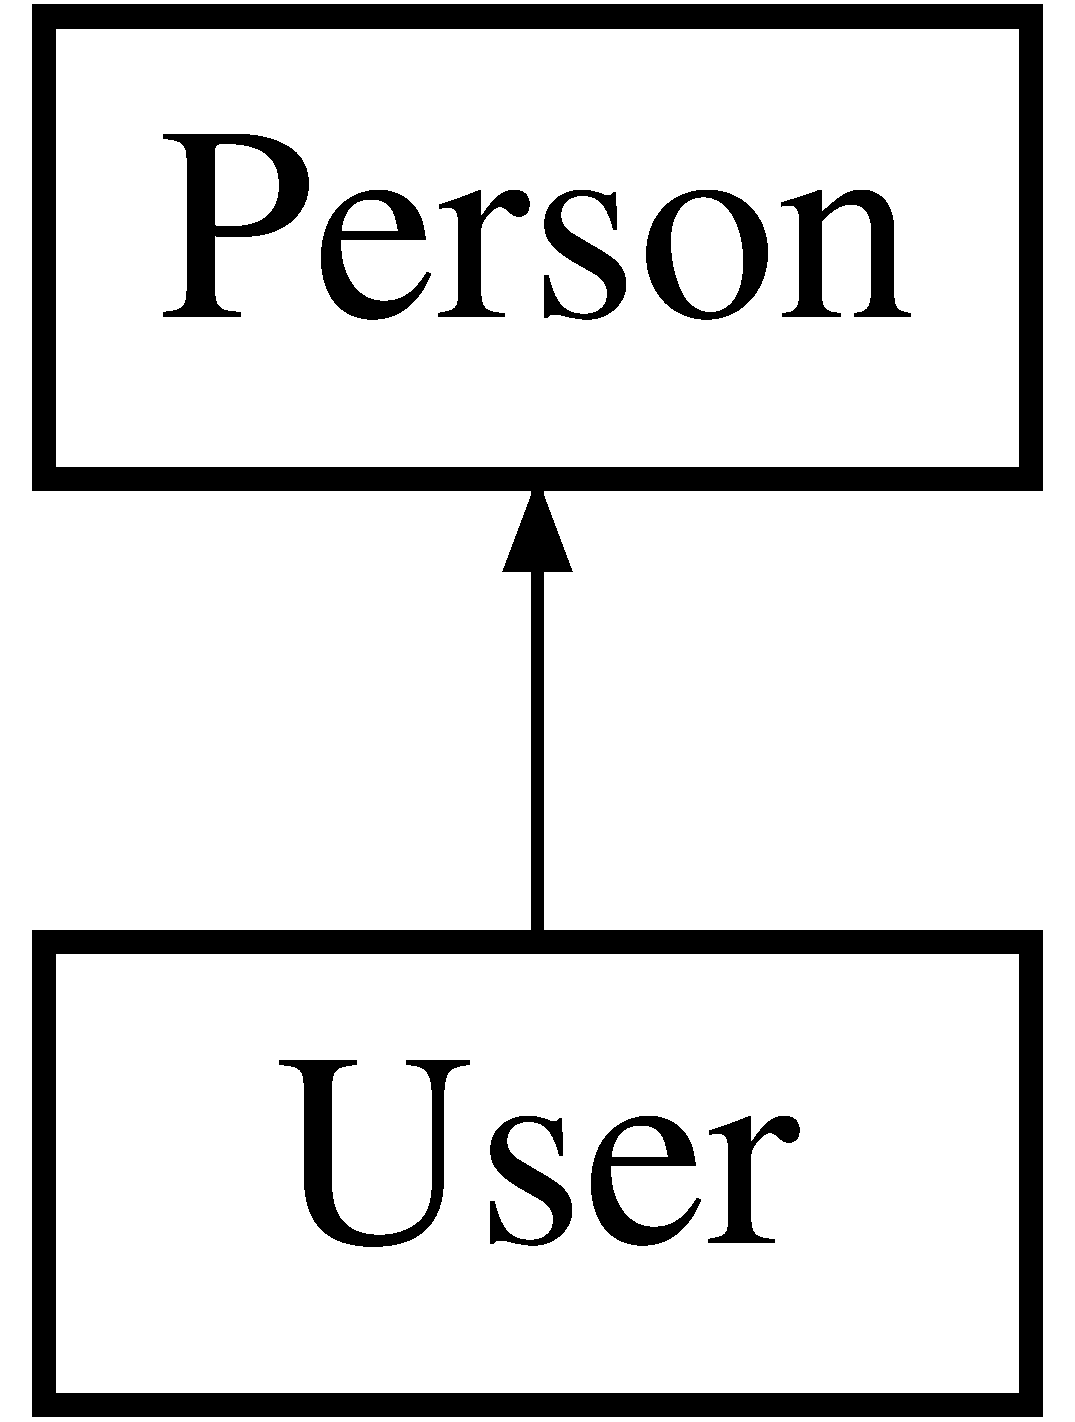
\includegraphics[height=2.000000cm]{class_user}
\end{center}
\end{figure}
\subsection*{Public Member Functions}
\begin{DoxyCompactItemize}
\item 
\mbox{\Hypertarget{class_user_a4a0137053e591fbb79d9057dd7d2283d}\label{class_user_a4a0137053e591fbb79d9057dd7d2283d}} 
\mbox{\hyperlink{class_user_a4a0137053e591fbb79d9057dd7d2283d}{User}} ()
\begin{DoxyCompactList}\small\item\em Constructor of the class. \end{DoxyCompactList}\item 
\mbox{\hyperlink{class_user_a898c6748faa70dcd3d30e550be2eb768}{User}} (std\+::string name, int age, std\+::string gender, bool is\+Gold, std\+::string assigned\+Teacher)
\begin{DoxyCompactList}\small\item\em Constructor of the class. \end{DoxyCompactList}\item 
\mbox{\Hypertarget{class_user_a1ddb4cbabc84ef92ac92bfe6f9385d39}\label{class_user_a1ddb4cbabc84ef92ac92bfe6f9385d39}} 
void \mbox{\hyperlink{class_user_a1ddb4cbabc84ef92ac92bfe6f9385d39}{make\+Gold}} ()
\begin{DoxyCompactList}\small\item\em Make a person have a Gold Card. \end{DoxyCompactList}\item 
\mbox{\Hypertarget{class_user_a88a8b41f134b21aeb702c481ffee0ef4}\label{class_user_a88a8b41f134b21aeb702c481ffee0ef4}} 
void \mbox{\hyperlink{class_user_a88a8b41f134b21aeb702c481ffee0ef4}{stop\+Gold}} ()
\begin{DoxyCompactList}\small\item\em Stop a person from having a Gold Card. \end{DoxyCompactList}\item 
bool \mbox{\hyperlink{class_user_ac1af1ded379bd2fd56f96f90348520fe}{getis\+Gold}} ()
\item 
\mbox{\hyperlink{class_report}{Report}} \mbox{\hyperlink{class_user_ad5f236ca0846ae3fc493609f72d17a70}{get\+Report}} (int month)
\item 
\mbox{\hyperlink{class_invoice}{Invoice}} \mbox{\hyperlink{class_user_a4fafb4511574972c6e7801f2bb6a638b}{get\+Invoice}} (int month)
\item 
std\+::vector$<$ \mbox{\hyperlink{class_invoice}{Invoice}} $\ast$ $>$ \mbox{\hyperlink{class_user_aeb297e5cd248e1e2c0ae3540cbedcca8}{get\+Invoices}} ()
\begin{DoxyCompactList}\small\item\em Getter of all the invoices. \end{DoxyCompactList}\item 
std\+::vector$<$ \mbox{\hyperlink{class_reservation}{Reservation}} $\ast$ $>$ \mbox{\hyperlink{class_user_a7443c5c7b1cca31c8400130568050327}{get\+Reservations}} ()
\begin{DoxyCompactList}\small\item\em Getter of all the \mbox{\hyperlink{class_reservation}{Reservation}}. \end{DoxyCompactList}\item 
std\+::string \mbox{\hyperlink{class_user_ac9fcbd4f944689de5faf746aa277d81a}{get\+Teacher}} ()
\begin{DoxyCompactList}\small\item\em Getter of the assigned teacher. \end{DoxyCompactList}\item 
void \mbox{\hyperlink{class_user_ad0432b83c7379ca57ed782d2929f3b8a}{set\+Invoice}} (\mbox{\hyperlink{class_invoice}{Invoice}} $\ast$invoice, int month)
\item 
void \mbox{\hyperlink{class_user_a0cdc359989bc67c3a135737cf1232a49}{set\+Report}} (\mbox{\hyperlink{class_report}{Report}} $\ast$report, int month)
\item 
void \mbox{\hyperlink{class_user_ab0e9dba3828977748ad6316eb346a854}{set\+Reservation}} (\mbox{\hyperlink{class_reservation}{Reservation}} $\ast$reservation)
\begin{DoxyCompactList}\small\item\em Setter of the reservation. \end{DoxyCompactList}\item 
void \mbox{\hyperlink{class_user_aac5ff0f6899f3ce56d1b2d12ed557c79}{store\+Info}} (std\+::ofstream \&outfile, int \&indentation)
\begin{DoxyCompactList}\small\item\em Store in the information of the \mbox{\hyperlink{class_user}{User}} to a file. \end{DoxyCompactList}\item 
void \mbox{\hyperlink{class_user_abc12a9ca668bd860a3d6d2ae4791997d}{load\+Class}} (std\+::ifstream \&inpfile)
\begin{DoxyCompactList}\small\item\em Reading the information of a \mbox{\hyperlink{class_user}{User}} from a file. \end{DoxyCompactList}\item 
\mbox{\Hypertarget{class_user_ac8a201055d02b313721e56c4c0f6af82}\label{class_user_ac8a201055d02b313721e56c4c0f6af82}} 
void \mbox{\hyperlink{class_user_ac8a201055d02b313721e56c4c0f6af82}{show}} ()
\begin{DoxyCompactList}\small\item\em Showing the information of the user on the screen. \end{DoxyCompactList}\item 
\mbox{\Hypertarget{class_user_a3ccbaec58dd37260a34dfa84496b30bd}\label{class_user_a3ccbaec58dd37260a34dfa84496b30bd}} 
void \mbox{\hyperlink{class_user_a3ccbaec58dd37260a34dfa84496b30bd}{clean\+Vectors}} ()
\begin{DoxyCompactList}\small\item\em cleaning all vectors inside the \mbox{\hyperlink{class_user}{User}} \end{DoxyCompactList}\item 
\mbox{\Hypertarget{class_user_ab0637e7ec103b32d040a0bc97be0f178}\label{class_user_ab0637e7ec103b32d040a0bc97be0f178}} 
void \mbox{\hyperlink{class_user_ab0637e7ec103b32d040a0bc97be0f178}{clean\+Reservations}} ()
\begin{DoxyCompactList}\small\item\em cleaning the Reservations \end{DoxyCompactList}\end{DoxyCompactItemize}


\subsection{Detailed Description}
The users of the court 

\subsection{Constructor \& Destructor Documentation}
\mbox{\Hypertarget{class_user_a898c6748faa70dcd3d30e550be2eb768}\label{class_user_a898c6748faa70dcd3d30e550be2eb768}} 
\index{User@{User}!User@{User}}
\index{User@{User}!User@{User}}
\subsubsection{\texorpdfstring{User()}{User()}}
{\footnotesize\ttfamily User\+::\+User (\begin{DoxyParamCaption}\item[{std\+::string}]{name,  }\item[{int}]{age,  }\item[{std\+::string}]{gender,  }\item[{bool}]{is\+Gold,  }\item[{std\+::string}]{assigned\+Teacher }\end{DoxyParamCaption})}



Constructor of the class. 


\begin{DoxyParams}{Parameters}
{\em name} & -\/ name of the person \\
\hline
{\em age} & -\/ age of the person \\
\hline
{\em gender} & -\/ gender of the person \\
\hline
{\em is\+Gold} & -\/ does the person have the Gold Card \\
\hline
{\em assigned\+Teacher} & -\/ the teacher assigned to the person \\
\hline
\end{DoxyParams}


\subsection{Member Function Documentation}
\mbox{\Hypertarget{class_user_a4fafb4511574972c6e7801f2bb6a638b}\label{class_user_a4fafb4511574972c6e7801f2bb6a638b}} 
\index{User@{User}!get\+Invoice@{get\+Invoice}}
\index{get\+Invoice@{get\+Invoice}!User@{User}}
\subsubsection{\texorpdfstring{get\+Invoice()}{getInvoice()}}
{\footnotesize\ttfamily \mbox{\hyperlink{class_invoice}{Invoice}} User\+::get\+Invoice (\begin{DoxyParamCaption}\item[{int}]{month }\end{DoxyParamCaption})}

Getter of the \mbox{\hyperlink{class_invoice}{Invoice}} of a Specific \mbox{\hyperlink{class_month}{Month}} 
\begin{DoxyParams}{Parameters}
{\em month} & -\/ month wanted \\
\hline
\end{DoxyParams}
\begin{DoxyReturn}{Returns}
the \mbox{\hyperlink{class_invoice}{Invoice}} of said month 
\end{DoxyReturn}
\mbox{\Hypertarget{class_user_aeb297e5cd248e1e2c0ae3540cbedcca8}\label{class_user_aeb297e5cd248e1e2c0ae3540cbedcca8}} 
\index{User@{User}!get\+Invoices@{get\+Invoices}}
\index{get\+Invoices@{get\+Invoices}!User@{User}}
\subsubsection{\texorpdfstring{get\+Invoices()}{getInvoices()}}
{\footnotesize\ttfamily vector$<$ \mbox{\hyperlink{class_invoice}{Invoice}} $\ast$ $>$ User\+::get\+Invoices (\begin{DoxyParamCaption}{ }\end{DoxyParamCaption})}



Getter of all the invoices. 

\begin{DoxyReturn}{Returns}
vector of Invoices 
\end{DoxyReturn}
\mbox{\Hypertarget{class_user_ac1af1ded379bd2fd56f96f90348520fe}\label{class_user_ac1af1ded379bd2fd56f96f90348520fe}} 
\index{User@{User}!getis\+Gold@{getis\+Gold}}
\index{getis\+Gold@{getis\+Gold}!User@{User}}
\subsubsection{\texorpdfstring{getis\+Gold()}{getisGold()}}
{\footnotesize\ttfamily bool User\+::getis\+Gold (\begin{DoxyParamCaption}{ }\end{DoxyParamCaption})}

Does this \mbox{\hyperlink{class_user}{User}} have a Gold Card \begin{DoxyReturn}{Returns}
if the user is gold 
\end{DoxyReturn}
\mbox{\Hypertarget{class_user_ad5f236ca0846ae3fc493609f72d17a70}\label{class_user_ad5f236ca0846ae3fc493609f72d17a70}} 
\index{User@{User}!get\+Report@{get\+Report}}
\index{get\+Report@{get\+Report}!User@{User}}
\subsubsection{\texorpdfstring{get\+Report()}{getReport()}}
{\footnotesize\ttfamily \mbox{\hyperlink{class_report}{Report}} User\+::get\+Report (\begin{DoxyParamCaption}\item[{int}]{month }\end{DoxyParamCaption})}

Getter of the \mbox{\hyperlink{class_report}{Report}} of a Specific \mbox{\hyperlink{class_month}{Month}} 
\begin{DoxyParams}{Parameters}
{\em month} & -\/ month wanted \\
\hline
\end{DoxyParams}
\begin{DoxyReturn}{Returns}
the report of said month 
\end{DoxyReturn}
\mbox{\Hypertarget{class_user_a7443c5c7b1cca31c8400130568050327}\label{class_user_a7443c5c7b1cca31c8400130568050327}} 
\index{User@{User}!get\+Reservations@{get\+Reservations}}
\index{get\+Reservations@{get\+Reservations}!User@{User}}
\subsubsection{\texorpdfstring{get\+Reservations()}{getReservations()}}
{\footnotesize\ttfamily vector$<$ \mbox{\hyperlink{class_reservation}{Reservation}} $\ast$ $>$ User\+::get\+Reservations (\begin{DoxyParamCaption}{ }\end{DoxyParamCaption})}



Getter of all the \mbox{\hyperlink{class_reservation}{Reservation}}. 

\begin{DoxyReturn}{Returns}
vector of Reservations 
\end{DoxyReturn}
\mbox{\Hypertarget{class_user_ac9fcbd4f944689de5faf746aa277d81a}\label{class_user_ac9fcbd4f944689de5faf746aa277d81a}} 
\index{User@{User}!get\+Teacher@{get\+Teacher}}
\index{get\+Teacher@{get\+Teacher}!User@{User}}
\subsubsection{\texorpdfstring{get\+Teacher()}{getTeacher()}}
{\footnotesize\ttfamily string User\+::get\+Teacher (\begin{DoxyParamCaption}{ }\end{DoxyParamCaption})}



Getter of the assigned teacher. 

\begin{DoxyReturn}{Returns}
the name of the teacher 
\end{DoxyReturn}
\mbox{\Hypertarget{class_user_abc12a9ca668bd860a3d6d2ae4791997d}\label{class_user_abc12a9ca668bd860a3d6d2ae4791997d}} 
\index{User@{User}!load\+Class@{load\+Class}}
\index{load\+Class@{load\+Class}!User@{User}}
\subsubsection{\texorpdfstring{load\+Class()}{loadClass()}}
{\footnotesize\ttfamily void User\+::load\+Class (\begin{DoxyParamCaption}\item[{std\+::ifstream \&}]{inpfile }\end{DoxyParamCaption})\hspace{0.3cm}{\ttfamily [virtual]}}



Reading the information of a \mbox{\hyperlink{class_user}{User}} from a file. 


\begin{DoxyParams}{Parameters}
{\em infile} & -\/ file to read the information from \\
\hline
\end{DoxyParams}


Reimplemented from \mbox{\hyperlink{class_person_af07a032df8d56dddade4dc43960b536b}{Person}}.

\mbox{\Hypertarget{class_user_ad0432b83c7379ca57ed782d2929f3b8a}\label{class_user_ad0432b83c7379ca57ed782d2929f3b8a}} 
\index{User@{User}!set\+Invoice@{set\+Invoice}}
\index{set\+Invoice@{set\+Invoice}!User@{User}}
\subsubsection{\texorpdfstring{set\+Invoice()}{setInvoice()}}
{\footnotesize\ttfamily void User\+::set\+Invoice (\begin{DoxyParamCaption}\item[{\mbox{\hyperlink{class_invoice}{Invoice}} $\ast$}]{invoice,  }\item[{int}]{month }\end{DoxyParamCaption})}

Setter of the \mbox{\hyperlink{class_invoice}{Invoice}} 
\begin{DoxyParams}{Parameters}
{\em invoice} & -\/ invoice to save \\
\hline
{\em month} & -\/ the month of the invoice \\
\hline
\end{DoxyParams}
\mbox{\Hypertarget{class_user_a0cdc359989bc67c3a135737cf1232a49}\label{class_user_a0cdc359989bc67c3a135737cf1232a49}} 
\index{User@{User}!set\+Report@{set\+Report}}
\index{set\+Report@{set\+Report}!User@{User}}
\subsubsection{\texorpdfstring{set\+Report()}{setReport()}}
{\footnotesize\ttfamily void User\+::set\+Report (\begin{DoxyParamCaption}\item[{\mbox{\hyperlink{class_report}{Report}} $\ast$}]{report,  }\item[{int}]{month }\end{DoxyParamCaption})}

Setter of the report 
\begin{DoxyParams}{Parameters}
{\em report} & -\/ report to save \\
\hline
{\em month} & -\/ the month of the report \\
\hline
\end{DoxyParams}
\mbox{\Hypertarget{class_user_ab0e9dba3828977748ad6316eb346a854}\label{class_user_ab0e9dba3828977748ad6316eb346a854}} 
\index{User@{User}!set\+Reservation@{set\+Reservation}}
\index{set\+Reservation@{set\+Reservation}!User@{User}}
\subsubsection{\texorpdfstring{set\+Reservation()}{setReservation()}}
{\footnotesize\ttfamily void User\+::set\+Reservation (\begin{DoxyParamCaption}\item[{\mbox{\hyperlink{class_reservation}{Reservation}} $\ast$}]{reservation }\end{DoxyParamCaption})}



Setter of the reservation. 


\begin{DoxyParams}{Parameters}
{\em reservation} & -\/ the reservation to save \\
\hline
\end{DoxyParams}
\mbox{\Hypertarget{class_user_aac5ff0f6899f3ce56d1b2d12ed557c79}\label{class_user_aac5ff0f6899f3ce56d1b2d12ed557c79}} 
\index{User@{User}!store\+Info@{store\+Info}}
\index{store\+Info@{store\+Info}!User@{User}}
\subsubsection{\texorpdfstring{store\+Info()}{storeInfo()}}
{\footnotesize\ttfamily void User\+::store\+Info (\begin{DoxyParamCaption}\item[{std\+::ofstream \&}]{outfile,  }\item[{int \&}]{indentation }\end{DoxyParamCaption})\hspace{0.3cm}{\ttfamily [virtual]}}



Store in the information of the \mbox{\hyperlink{class_user}{User}} to a file. 


\begin{DoxyParams}{Parameters}
{\em outfile} & -\/ the file to write information \\
\hline
{\em indent} & -\/ current indentation \\
\hline
\end{DoxyParams}


Reimplemented from \mbox{\hyperlink{class_person_a80f87df3f644706c2ad8fc8b800fdd95}{Person}}.



The documentation for this class was generated from the following files\+:\begin{DoxyCompactItemize}
\item 
Person.\+h\item 
Person.\+cpp\end{DoxyCompactItemize}

\hypertarget{class_year}{}\section{Year Class Reference}
\label{class_year}\index{Year@{Year}}


{\ttfamily \#include $<$Calendar.\+h$>$}

\subsection*{Public Member Functions}
\begin{DoxyCompactItemize}
\item 
\mbox{\hyperlink{class_year_af5910fa97849bd9b700262477fd1fd24}{Year}} ()
\begin{DoxyCompactList}\small\item\em Class Constructor. \end{DoxyCompactList}\item 
\mbox{\hyperlink{class_year_ac18a4f513e8ee98b352990c6f54bd663}{Year}} (int year)
\begin{DoxyCompactList}\small\item\em Class Constructor. \end{DoxyCompactList}\item 
\mbox{\hyperlink{class_month}{Month}} \& \mbox{\hyperlink{class_year_a64bc478fe629fc966b7bfadb1d939a88}{get\+Month}} (int month)
\begin{DoxyCompactList}\small\item\em Getter of the month. \end{DoxyCompactList}\item 
void \mbox{\hyperlink{class_year_a1478407d9100f722e54daaf1ce2a413c}{set\+Months}} (std\+::vector$<$ \mbox{\hyperlink{class_month}{Month}} $>$ months)
\begin{DoxyCompactList}\small\item\em Setter of the months. \end{DoxyCompactList}\end{DoxyCompactItemize}


\subsection{Detailed Description}
The year with all of its months 

\subsection{Constructor \& Destructor Documentation}
\mbox{\Hypertarget{class_year_af5910fa97849bd9b700262477fd1fd24}\label{class_year_af5910fa97849bd9b700262477fd1fd24}} 
\index{Year@{Year}!Year@{Year}}
\index{Year@{Year}!Year@{Year}}
\subsubsection{\texorpdfstring{Year()}{Year()}\hspace{0.1cm}{\footnotesize\ttfamily [1/2]}}
{\footnotesize\ttfamily Year\+::\+Year (\begin{DoxyParamCaption}{ }\end{DoxyParamCaption})\hspace{0.3cm}{\ttfamily [inline]}}



Class Constructor. 

\mbox{\Hypertarget{class_year_ac18a4f513e8ee98b352990c6f54bd663}\label{class_year_ac18a4f513e8ee98b352990c6f54bd663}} 
\index{Year@{Year}!Year@{Year}}
\index{Year@{Year}!Year@{Year}}
\subsubsection{\texorpdfstring{Year()}{Year()}\hspace{0.1cm}{\footnotesize\ttfamily [2/2]}}
{\footnotesize\ttfamily Year\+::\+Year (\begin{DoxyParamCaption}\item[{int}]{year }\end{DoxyParamCaption})}



Class Constructor. 


\begin{DoxyParams}{Parameters}
{\em year} & -\/ current year \\
\hline
\end{DoxyParams}


\subsection{Member Function Documentation}
\mbox{\Hypertarget{class_year_a64bc478fe629fc966b7bfadb1d939a88}\label{class_year_a64bc478fe629fc966b7bfadb1d939a88}} 
\index{Year@{Year}!get\+Month@{get\+Month}}
\index{get\+Month@{get\+Month}!Year@{Year}}
\subsubsection{\texorpdfstring{get\+Month()}{getMonth()}}
{\footnotesize\ttfamily \mbox{\hyperlink{class_month}{Month}} \& Year\+::get\+Month (\begin{DoxyParamCaption}\item[{int}]{month }\end{DoxyParamCaption})}



Getter of the month. 


\begin{DoxyParams}{Parameters}
{\em month} & -\/ the month wanted \\
\hline
\end{DoxyParams}
\begin{DoxyReturn}{Returns}
the month 
\end{DoxyReturn}
\mbox{\Hypertarget{class_year_a1478407d9100f722e54daaf1ce2a413c}\label{class_year_a1478407d9100f722e54daaf1ce2a413c}} 
\index{Year@{Year}!set\+Months@{set\+Months}}
\index{set\+Months@{set\+Months}!Year@{Year}}
\subsubsection{\texorpdfstring{set\+Months()}{setMonths()}}
{\footnotesize\ttfamily void Year\+::set\+Months (\begin{DoxyParamCaption}\item[{std\+::vector$<$ \mbox{\hyperlink{class_month}{Month}} $>$}]{months }\end{DoxyParamCaption})}



Setter of the months. 


\begin{DoxyParams}{Parameters}
{\em months} & -\/ vector of months \\
\hline
\end{DoxyParams}


The documentation for this class was generated from the following files\+:\begin{DoxyCompactItemize}
\item 
\mbox{\hyperlink{_calendar_8h}{Calendar.\+h}}\item 
\mbox{\hyperlink{_calendar_8cpp}{Calendar.\+cpp}}\end{DoxyCompactItemize}

%--- End generated contents ---

% Index
\backmatter
\newpage
\phantomsection
\clearemptydoublepage
\addcontentsline{toc}{chapter}{Index}
\printindex

\end{document}
